%
% 
% Release of skeleton 2017/11/24, Alejandro
%
%
%\documentclass[11pt,twoside,titlepage]{article}
\documentclass[11pt]{article}
\usepackage{a4,amssymb,rotating}
\usepackage{epsfig,subfigure,fancyheadings}
\usepackage{graphicx,color}
\usepackage{lineno}

\setlength{\oddsidemargin}{+0.3cm}
\setlength{\evensidemargin}{-0.3cm}
\setlength{\textwidth}{15.5cm}
\setlength{\textheight}{22.5cm}
\setlength{\topmargin}{-2.0cm}

\newif\ifcomment
\commenttrue % comment to remove comments

\newif\iflinenumber
\linenumbertrue % comment to remove line numbering

\newcommand{\comment}[1]{\ifcomment \color{blue}{\underline{Comment:} #1}\color{black}\fi}
%\newcommand{\guari}{G\"UARIG\"UANCHI}
\newcommand{\guari}{GUARIGUANCHI}
\newcommand{\todo}{{\bf \color{red} NOTE: This feature is still waiting for implementation!!!}}

\begin{document}
\sloppy 
% \linenumbers

\title{{\bf User Manual}}

\author{A.~P\'erez~P\'erez\\
~\\
{\it\footnotesize PICSEL Group, IPHC - CNRS} \\
{\it\footnotesize 23 rue du Loess 67037 Strasbourg, France}\\
}

\date{November 2017}

% \comment{There will be a front page with AIDA logo and format}

\begin{figure}
  \centering
  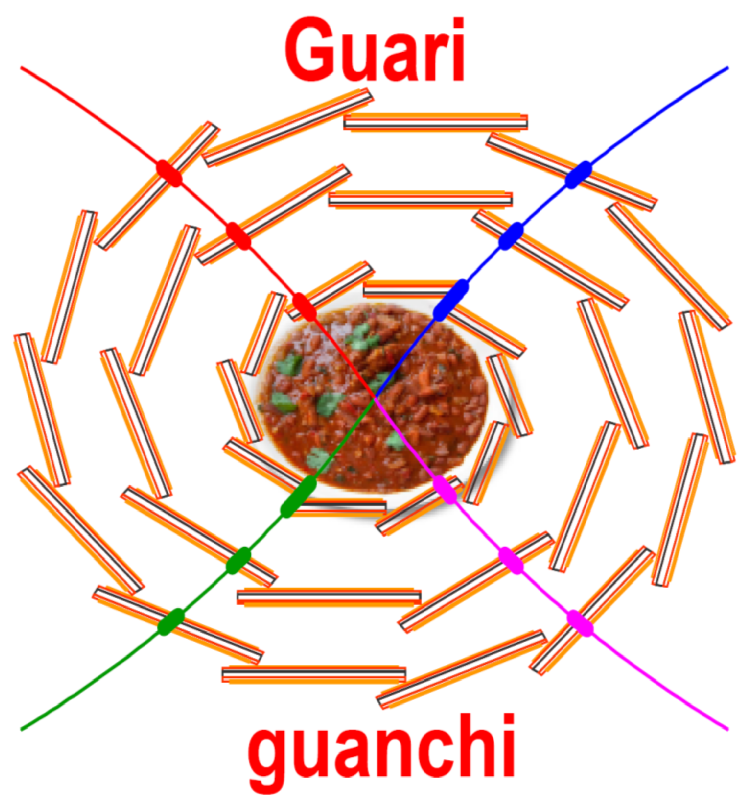
\includegraphics[width=0.7\textwidth]{figures/Guariguanchi_logo.png}
\end{figure}

\maketitle

\newpage

\begin{abstract}
{\guari} is a tool for a simplified calculation of tracking performances which is fast and can be used as an intermediate step in the process 
of tracking system optimization. It allows to quickly compare different detector geometries as well as combinations of sensor performances
leading to a reduced set of configurations for deeper studies with full-simulation. The tool also allows to optimize beam-test setups in 
terms of telescope pointing resolution at the device under test location. This document is intended to present the basis to install and start 
using \guari. The document also provides all the information about the code structure and presents guide-lines on how to extend it.
\end{abstract}

\newpage

\tableofcontents

\newpage

\section{Introduction}
\label{sec:Intro}

{\guari} is a package created in the context of the ILD collaboration~\cite{bib:ILDcoll} and managed by the PICSEL group at IPHC (Strasbourg).
It actually started as a tool for calculating telescope's pointing resolution at device under test (DUT) position for beam-test setups. It then quickly 
transformed for the more challenging task of tracker optimization by comparing tracking performances of different detector configurations.

The package has a set of tools which allows to calculate for a given momentum $(p,\theta,\phi)$ the track parameters covariance matrix. It also allows to 
calculate a tracking efficiency with simplified pattern recognition algorithms. The details of the calculations are explained in section~\ref{sec:Math_formalism}.
Of course, these calculations are performed with simplifying assumptions and ignore other effects that can only be taken into account with full-simulation 
and realistic pattern recognition algorithms. Detector optimization can be guided by plotting the tracking performances as a function momentum, polar and 
azimuthal angles for the different detector configurations.

\subsection{General philosophy}

{\guari} is a C++ software meant as a lightweight package in which only {\tt ROOT}~\cite{bib:root} pre-installation is required. During installation an executable 
is produced which is later run with a configuration data-card. This data-card contains all the configuration variables for the analyses to be performed on a list of 
geometries. The work-flow is as follows,

\begin{itemize}

 \item  Readout of the analysis configuration variables, {\it e.g.} particle type and origin, momentum ranges in terms of $(p,\theta,\phi)$, 
 analysis variables, and list of geometry data-cards (geo-datacard).
 
 \item  Geometries build-up. The geo-data-cards are readout to build a list of geometries.
 
 \item  Each geometry has a so-called tracker associated to it. This object is the one able to perform all the tracking performances 
 calculations related with the geometry, {\it e.g.} track intersections with geometry (including sensitive and insensitive elements), space points 
 covariance matrix (including multiple scattering and energy loss fluctuations), track parameters covariance matrix and tracking efficiency.
 
 \item  Depending of the analysis configuration, different plots can be produced: geometry visualization (including some tracks if specified), 
 track parameters resolution  and/or tracking efficiency vs $(p,\theta,\phi)$.
 
\end{itemize}

The resulting plots are always stored in a multiple pages pdf file, and can if requested be stored in an output root file as well.

\section{Getting Started}
\label{sec:Getting_started}

\subsection{Installation}

{\guari} has been fully tested with {\tt ROOT} version 5.34/32 and is expected to work with higher versions. To install {\guari} 
you will need to go to the following website: FFFFF. By clicking at the XXX link you will download a {\tt guariguanchi.tar.gz} file. 
Unpack it with the following command,

~\\
\noindent
{\tt >\$ tar -xzvf guariguanchi.tar.gz}
~\\

\noindent
Then go to the {\tt Guariguanchi} directory and simply do,

~\\
\noindent
{\tt >\$ ./Compile.sh}
~\\

\noindent
It should produce a list compiled objects ({\tt .o} files) inside the {\tt lib/} directory, as well as an executable inside the {\tt bin/} 
directory called {\tt GuariguanchiApp}. If you get some compilation errors you maybe need to verify the options during your {\tt ROOT} build-up. 

% The details of the calculations are explained in section~\ref{sec:Math_formalism}.

\subsection{Playing with some examples}
\label{subsec:Some_examples}

Once the package is compiled it is quite simple to use. You just need to get a data-card ({\tt datacard.txt}) and run {\guari} as 
follows,

~\\
\noindent
{\tt >\$ ./bin/GuariguanchiApp  datacard.txt}
~\\

\noindent
Now let's play with some examples and discover the package in the process.

\subsubsection{Example-1: Beam-test}
\label{subsubsec:Example1}

This example consist on a classic beam-test configuration, in which only straight tracks will be considered (no magnetic field). 
What is mainly needed in this analysis is the telescope pointing resolution at the DUT's positions. All the data-cards for this 
example can be found at the directory, 

~\\
{\tt DataCards/Examples/BeamTest\_Example/}.
~\\

\noindent
Lets open the main data-card, {\tt BeamTest\_datacard.txt}, and take a look at it. The configuration is specified with a list of 
parameters blocks which will be described here below (for a complete description of all the possible parameters specified in the 
main data-card see sec.~\ref{sec:analysis_config}).

\begin{itemize}
 \item  {\tt ParticleType:} in the present case we consider an electron ({\tt e-}).
 
 \item  {\tt ParticleOrigin:} point from which the particle will be tracked in the process of geometry navigation. Current value is $(0,0,-1)~{\rm cm}$.
 
 \item  {\tt ReferencePoint:} pivot-point for trajectory parameterization. Current value is $(0,0,10)~{\rm cm}$.
 
 \item  The momentum values are specified as a set of $(p,\theta,\phi)$ values. In the current case 
 
  \begin{itemize}
   \item  $p$-values: range inside the {\tt BeginMomentumScan} and {\tt EndMomentumScan} bock $\Rightarrow$ 30 bins between $1$ and $40$ ${\rm GeV/c}$.
   
   \item  $\theta$-values: set of discrete values $\Rightarrow$ single value of $0~{\rm deg}$.
   
   \item  $\phi$-values: set of discrete values $\Rightarrow$ single value of $0~{\rm deg}$.
  \end{itemize}
  
  \item {\tt TrkResolAnalysisParams} block. In the present case we are going to study the telescope resolution at DUT positions. The configuration for 
  this analysis is specified inside the block between {\tt BeginTrkResolAnalysisParams} and {\tt EndTrkResolAnalysisParams}. Only three parameters are 
  specified in this case.
  
  \begin{itemize}
   \item  {\tt NhitsMin}: minimum number of hits for a track. In this case it is set to 2 (minimum number of hits to reconstruct a straight line).
   
   \item  {\tt SameRange}: flag to use same vertical range for all plots. Set to {\tt false} in this case. 
   
   \item  {\tt UseAllMomVals}: flag to use all specified momentum values for additional plots. Set to {\tt true} in this case.
  \end{itemize}
  
  \item  The list of geometries is specified inside the block between {\tt BeginGeometries} and {\tt EndGeometries}. In there the list of geo-data-cards is specified.
  In the current case four geometries are given.
  
  \item  {\tt OutputFile:} output file generic name (no extension). The output of the program will generate a set of output files with the specified generic name 
  plus the corresponding extension, {\it e.g.} {\tt .pdf} and/or {\tt .root}.
  
  \item  Finally a set of flags will determine the output plots and files. In the current example we have,
  
  \begin{itemize}
   \item  {\tt PrintGeometry:} print-out of all specified geometries.
   \item  {\tt PlotGeometry:} visualization of all specified geometries.
   \item  {\tt PlotWorldVolume:} if {\tt PlotGeometry} is set to {\tt true} will also visualize geometry's world volume.
   \item  {\tt DoTelescopeAnalysis:} flag to perform a Telescope analysis.
   \item  {\tt SavePlots:} flag to save plots in a {\tt .root} output file.
  \end{itemize}
  
\end{itemize}

\noindent
Now lets run this example as follows,

~\\
\noindent
{\tt >\$ ./bin/GuariguanchiApp  fullpath/BeamTest\_datacard.txt}
~\\

\noindent
where {\tt fullpath} is the full path to the main data-card location.
The execution should take about 20 seconds. You should see a lengthy printout with all the geometries ({\tt PrintGeometry} set to {\tt true}). 
It also produced two output files, one {\tt .pdf} and one {\tt .root}, inside the {\tt Plots/Examples/BeamTest\_Example/} output directory. 
Lets open the {\tt .pdf} file. This is a multi-page file with several plots.

The first four pages is a visualization of the four specified geometries. The geometries are projected in the $Z-Y$, $Z-X$ 
and $X-Y$ planes. We can see 9 yellow elements, which are silicon planes. Six of them are the telescope planes (big ones located between 
$(0,10)~{\rm cm}$ and $(10,20)~{\rm cm}$ in $Z$). The smaller planes are DUT-1,2 and 3, located at $Z = 0,10,20~{\rm cm}$, respectively. 
The red-dotted line represents the geometry's world volume, which in this case is a box. It can be seen that the only change from one 
geometry to the next are the locations of the telescope planes.

The 5th page shows the track's parameters resolution vs momentum for the only $(\theta,\phi) = (0,0)~{\rm deg}$ value specified. As there is no 
magnetic field the trajectories are straight lines, needing only four parameters defined at the pivot point: ${\rm tan}(\alpha_{x})$, $x_{0}$, 
${\rm tan}(\alpha_{y})$ and $y_{0}$. The color code is described in the legend at the bottom-right part of the page, each color corresponding to 
one of the specified geometries. The momentum-dependence of tracking performances is due to the multiple-scattering (MS), which decreases as 
momentum increases.

The last three pages show the telescope pointing resolution at the DUT positions vs momentum. The plots on the top show the telescope 
pointing resolution on the DUT-plane local $U$ and $V$ coordinates, top-left and top-right plots, respectively. The bottom-left
plot shows the $1-\sigma$ area $S$ (taking correlations into account) of the telescope's pointing resolution. Finally, the bottom-right 
plot shows the number of background hits in this $S$ surface calculated using the DUT's readout time $t_{\rm r.o.}$ and background level 
$R_{\rm bkg}$ (hits per unit time per unit surface) as follows,

\begin{equation}
 {\rm N_{bkg}} = S \times t_{\rm r.o.} \times R_{\rm bkg}.
\end{equation}
\noindent
This last quantity is useful in studying the probability of wrong hit association in tracking pattern recognition.

~\\
\noindent
Just to finalize discussing this example lets explore the geo-data-cards. All the data-cards are inside the directory 

~\\
\noindent
{\tt DataCards/Examples/BeamTest\_Example/GeometryCards/} 
~\\

\noindent
All are very similar, so it will be enough to take a look of just one of them, {\it e.g.} {\tt BeamTestGeometry\_v1.txt}. It 
starts with the specification of the geometry name {\tt GeometryName:}, followed by a set of input files ({\tt InputFile:}) 
in which different aspects of the geometry are specified. The content of the input files could directly be written inside 
the geo-data-card, but this modularity has the advantage to simplify the reading of the geometry as well as allows to specify 
just once aspects shared by different geometries.

In this example each geo-data-card has four input files, three of them being common to all. The content of the input files is the following,
\begin{itemize}
 \item  {\bf Geometry's world volume:} It is a volume which contains all the elements of a geometry. In the current case it is just a box 
 located at the origin and with widths $(W_x,W_y,W_z) = (3,4,22)~{\rm cm}$. 
 
 \item  {\bf DUT planes:} this file contains the set of DUT planes. Each one is a geometry-object called {\tt GeoPlane}, corresponding to so-called 
 "planes", which are boxes with one of the dimensions being small compared to the others two. The variables inside the block between {\tt BeginGeoPlane} and {\tt EndGeoPlane} are 
 self evident. More details will be given in sec.~\ref{sec:GeoConf}. Just note that the in this file there are specified three 
 DUT planes, with thicknesses of $50~{\rm \mu m}$, widths of $(W_u,W_v) = (1,1)~{\rm cm}$, parallel to the $X-Y$ plane and located at 
 $(X,Y) = (0,0)$ and $Z = 0,10,20~{\rm cm}$, respectively. For the beam-telescope analysis one important variable is the {\tt LayerName},
 which will be used to identify the planes as DUTs.
 
 \item  {\bf Telescope planes:} each element in this input file is a {\tt GeoPlane} object. Six planes are specified 
 with thicknesses of $50~{\rm \mu m}$, widths of $(W_u,W_v) = (2,3)~{\rm cm}$, parallel to the $X-Y$ plane and located at $(X,Y) = (0,0)$ and 
 $Z = 1,3,5,15,17,19~{\rm cm}$, respectively. As in the case of the DUT planes, one important variable is the {\tt LayerName}, which will be 
 used to identify the telescope planes. The other geometries differ in the position of the telescope planes.
 
 \item  {\bf Beam-Test configuration:} in this file the telescope and DUT planes are identified. It is done by specifying inside the block between
 {\tt BeginBeamTestConfiguration} and {\tt EndBeamTestConfiguration} the list of telescope planes ({\tt TelescopeLayersList}) and DUT planes 
 ({\tt DUTLayersList}). This is how the analysis knows which planes are going to be used for tracking (telescope) and which ones considered 
 as DUTs. If there is any other geometry-object not belonging to the telescope or DUT list, it will be considered as a insensitive element 
 only contributing to multiple-scattering.
 
\end{itemize}

\noindent
The output {\tt .root} file contains a set of canvases and {\tt TGraph} objects. By their naming it is self evident what they are. We strongly recommend 
the user to open this file with {\tt ROOT} and plot its contents.

~\\
\noindent
Something that should have been noticed by now is that {\guari} has a unit system. This is why all the specified quantities have to 
be accompanied of the corresponding units. Furthermore, in the data-cards files all contents after a double-slash "//" are considered as 
commentary and not readout.

\subsubsection{Example-2: All-silicon vertex detector \& tracker}
\label{subsubsec:Example2}

This example considers an all-silicon vertex detector and tracker with cylindrical detection layers similar to the design of the ALICE 
Inner-Tracking-System upgrade~\cite{bib:ALICE_ITS_Upgrade}. The system is inside a solenoidal magnetic field of $0.5~{\rm Tesla}$ along the 
$z$-axis. In this case particles will describe Helix trajectories, which can be described with 5 parameters. In this package we use 
the same parameters as in Belle~\cite{bib:BelleHelixParam}: $d_{\rho}$, $d_z$, $\phi_0$, $tan\lambda$ and signed $p_t$. All the data-cards 
for this example can be found at the directory, 

~\\
{\tt DataCards/Examples/VertexDetector\_and\_Tracker\_Example/}.
~\\

\noindent
As you can notice, there are four main data-cards. Each one of them will serve to illustrate different analyses that can be performed with this 
package, and will be discussed in the following. 

\subsubsection*{Geometry visualization}

Lets start with a simple visualization of the geometries. For this lets open the data-card with the name

~\\
{\small{\tt VertexDetector\_and\_Tracker\_datacard\_GeometryVisualization.txt}}.
~\\

Much of the parameters in this file have already been described in the previous example (c.f. sec.~\ref{subsubsec:Example1}). 
In this case we consider $\mu^{+}$ as primary particles created at the origin, the pivot point is also fixed at the origin, 
and the momentum variables are specification in the same way as in the previous example. Two geometries are considered here. 
In order to visualize them just execute {\tt ./bin/GuariguanchiApp} with this data-card. The list of analysis flags set to {\tt true} 
in the main data-card should give an idea of what is going to be the output of this command,

\begin{itemize}
 \item  {\tt PrintGeometry:} print out of the geometries.
 
 \item  {\tt PrintGeometryWeight:} print out of the geometries weight. As can be seen, the weight are separated by systems. The 
 total weight is also printed-out.
 
 \item  {\tt PlotGeometry:} a visual representation similar to the previous example will be created. If this variable is set to {\tt true},
 other options can be considered.
 \begin{itemize}
  \item  {\tt PlotWorldVolume:} a visual representation of the geometry's world volume will be created.
  \item  {\tt DoRZGeoRepresentation:} a $R-Z$ representation of the geometry will be created. This representation is useful for 
  geometries with cylindrical symmetry with respect to the z-axis.
  \item  {\tt PlotSomeTracks:} for each value of $(\theta,\phi)$ specified a set of particle's average trajectories (no MS) as well as 
  their intersections with the geometry will be displayed.
 \end{itemize}

 \item  {\tt SavePlots:} as in the previous example, a {\tt .root} file will be created.
\end{itemize}

Given the options above, a {\tt .pdf} and {\tt .root} files are crated. The {\tt .pdf} file is again a mult-page file with several plots. 
Pages 1 and 2 show a visualization of the first geometry specified (Vertex \& Tracker Setup v1). Page 1 shows a visualization on the $Y-Z$, 
$X-Z$ and $X-Y$ planes of the geometry. Page 2 shows a $R-Z$ representation of the geometry. It can be seen that this geometry is mainly 
made of cylinders of different radii and lengths. The innermost one in green is a representation of a beam-pipe, made of beryllium. The yellow 
cylinders are the layers of the vertex detector and tracker, seven $50~{\rm \mu m}$ thickness silicon layers. Finally, the dotted-red 
line is a representation of the geometry's world volume. Pages 3 and 4 show similar visualizations for the second geometry specified (Vertex \& 
Tracker Setup v2). The difference of this last geometry with the first one is the radius and length of the 3rd tracker layer.

Pages 5-10 show a display of the first geometry with a set of track superimposed. Each set of plots corresponds to a fixed value of the specified
$(\theta,\phi)$ (see plot titles). The different colors correspond to the momenta specified in the legend box, which is a set of 10 values 
between the minimum and maximum specified momenta in the main data-card. The intersections of the tracks with the geometries are also shown 
(filled-circular-dots). Pages 11-16 show similar plots for the second geometry.

The output {\tt .root} file contains a set of canvases with the same geometry representations, which can be manipulated by the user in order to 
better understand the geometry as well as tracks intersections with geometries.

This geometry visualization feature is very useful in the process of building a geometry, as well as to understand the tracking performances, as 
it depends on the track intersections with sensitive layers (number of hits) and insensitive elements (material budget) of the geometry elements. 

~\\
Before exploring the other analyses data-cards, lets take a look of the geo-data-cards which are inside the {\tt GeometryCards} directory. The 
configuration files of both geometries are very similar, so it will be enough to take a look of one of them, {\it e.g.} {\tt Si\_Tracker\_Geometry\_v1.txt}.

The first parameter specified is the geometry name ({\tt GeometryName:}). As in the previous example, there is a set of input files, each one describing 
one feature of the geometry,

\begin{itemize}
 \item  {\bf Geometry's world volume:} in this case it is a cylinder centered at the origin and with radius and length of $50~{\rm cm}$ and $170~{\rm cm}$, 
 respectively.
 
 \item  {\bf Magnetic field:} a constant magnetic field of magnitude of $0.5~{\rm Tesla}$ and along the positive z-axis.
 
 \item  {\bf Beam-pipe:} a cylinder ({\tt GeoCylinder} object) made of beryllium centered at the origin, with radius, length and thickness of $1.96~{\rm cm}$, $20~{\rm cm}$ and $0.8~{\rm mm}$, 
 respectively. Notice that the {\tt LayerName} has been set to "Beam-Pipe". It will be used later to define the different systems of the geometry.
 
 \item  {\bf The Tracker:} a set of 7 cylinders ({\tt GeoCylinder} objects), all made of silicon with $50~{\rm \mu m}$ thickness at different radii and lengths. All of 
 them also share the same single point resolution ({\tt ResolutionU} and {\tt ResolutionV}), readout time ({\tt ROtime}) and detection efficiency ({\tt Efficiency}) 
 of $4~{\rm \mu m}$, $10~{\rm \mu s}$ and $99~\%$, respectively. Notice the value of the {\tt LayerName} variable. It will be used later to setup a telescope-DUT 
 configuration as well as to define the different systems of the geometry.
 
 \item  {\bf Telescope-DUT config:} this file is similar to the corresponding one of the previous example. In this case the innermost layer is considered as DUT 
 and all the rest as telescope.
 
 \item  {\bf Systems definition:} this is a new feature in which different "layers" can be put together to define a system. In this example there are three 
 systems defined,
 \begin{itemize}
  \item  Beam-Pipe system: including the beam-pipe;
  
  \item  Tracker-Inner Barrel: including the three innermost tracker layers;
  
  \item  Tracker-Outer Barrel: including the four outermost tracker layers.
 \end{itemize}
  This system definition can be useful to perform material budget analyses as well as performing cut for good tracks when doing
  efficiency calculations.
  
  \item  {\bf Track-Finding lagorithms:} this file contains all the needed information for the tracking efficiency calculation. A list of so-called 
  track-finder algorthms will be specified for different regions in the particle's origin and momenta. A track finder algorithm is specified in the 
  block between {\tt BeginXXXTrackFinderAlgo} and {\tt EndXXXTrackFinderAlgo}, where {\tt XXX} refers to a given track-finder algorithm. In the current 
  case it is used the FPCCD track-finder ({\tt FPCCDTrackFinderAlgo}), one of the pattern recognition algorthms used by the ILD collaboration~\cite{bib:ILD_FPCCD_TrackFinder}.
  
  The region where this track-finder will be applied is defined in the block between {\tt BeginTrackFinderRegion} and {\tt EndTrackFinderRegion}. In 
  the current case it corresponds momentum $\theta$ range between $(25.0,110.0)~{\rm deg}$.
  
  The "parameters" of this tracking finder are listed below,
  \begin{itemize}
    \item  {\tt NhitsMin}: minimum number of hits.
    
    \item  {\tt PtMin}: minimum transverse momentum cut for track-seeding.
    
    \item  {\tt CenterPosition:} coordinates of the track-center used for the minimum track-seeding cut.
    
    \item  {\tt PurityMin}: minimum track purity, defined as the ratio (\# good hits)/(\# total hits). This allows for a number of so-called fake 
    hits associated to the track.
    
    \item  {\tt NfakesMaxSeeding}: maximum number of fake hits for track-seeding. This parameter can take either the values 0 or 1.
    
    \item  {\tt Chi2OndfSeed}: $\chi^2$ cut for seed tracking.
    
    \item  {\tt Chi2OndAdd}: $\chi^2$ cut for hit-track association in the process of inward tracking.
    
    \item  {\tt InwardTracking}: bool parameter to define the tracking direction, either inward or outward.
    
    \item  {NmcSeedEffic}: number of samplings for a MC calculation of the seeding probability.
  \end{itemize}
  
  The list of geometry elements to be considered in the tracking efficiency calculation is defined by specifying a list of systems inside the {\tt BeginSystems} and {\tt EndSystems} block.
  This allows to use a sub-set of the tracking system for tracking efficiency calculation. In the current case all the systems are considered.
  
  Finally, a list of so-called "seeding configurations" are specified in the block inside {\tt BeginSeedConfigs} and {\tt EndSeedConfigs}. Each element is a set of 3 {\tt LayerNames} to be 
  used as a seed.
  
  More detail about the configuration of a track-finder algorithm can be found in sec.~\ref{subsec::TrkFinder_config} and a full explaination of the formalism for the tracking efficiency calculation 
  is is given in sec.~\ref{subsec:TrkEffic_calculation}.
  
\end{itemize}

\subsubsection*{Tracking resolution analysis}

The data-card for this analysis is the one with the name

~\\
{\small {\tt VertexDetector\_and\_Tracker\_datacard\_TrackerResolution.txt}}.
~\\

\noindent
It is very similar to the one for geometry visualization. The main difference is the specification of the {\tt TrkResolAnalysisParams} block and a set of different flags set to {\tt true}
at the end of the file. In this case the {\tt NhitsMin} is set to 3 (the minimum number of hits to reconstruct a helix), and a new flag {\tt UseLogY} is used and set to {\tt true}. 
This is only to use a logarithmic scale in the vertical axis of the track performances plots that will be produced. If not specified or set to {\tt false} a linear scale will be used instead.

Only two flags are set to {\tt true} at the end of the file, {\tt SavePlots} and {\tt DoTrkResolAnalysis}. This last one is for turning-on the tracking resolution analysis. This 
analysis will produce plots of the resolution on the track parameters vs momentum. The tracking calculation will be performed using all the track intersections with the geometry's 
sensitive elements. Lets execute this analysis as follows,

~\\
{\small {\tt ./bin/GuariguanchiApp  fullpath/VertexDetector\_and\_Tracker\_datacard\_TrackerResolution.txt}}.
~\\

\noindent
A {\tt .pdf} and {\tt .root} files have been produced. The {\tt .pdf} file have several pages showing the resolution of track parameters vs momentum: $\sigma(d_{\rho})$ (top-left),
$\sigma(\phi_0)$ (top-middle), $\sigma(d_z)$ (top-right), $\sigma(tan\lambda)$ (bottom-left) and $\sigma(p_{t})/p_{t}$ (bottom-middle). The color code is explained at the bottom-right 
legend, each one corresponding to the geometries specified. A vertical logarithmic scale is used as the {\tt UseLogY} parameter have been set to {\tt true} inside the {\tt TrkResolAnalysisParams} 
block in the main data-card file. Each page of this file show the tracking performances vs momentum for each of the $(\theta,\phi)$ values specified in the main data-card.

The {\tt .root} file content is self-explaining. We strongly advice the user to plot its contents.

\subsubsection*{Telescope analysis}

The data-card for this analysis is the one with the name

~\\
{\small {\tt VertexDetector\_and\_Tracker\_datacard\_TelescopeAnalysis.txt}}.
~\\

\noindent
It is very similar to the one of the Tracking resolution analysis, the only difference being the analysis flag set to {\tt true} at the end of the data-card, {\tt DoTelescopeAnalysis}. 
An analysis similar to the one of the beam-test configuration, with the only difference that in this case the tracks wont be straight but helices. Lets execute it as follows,

~\\
{\small {\tt ./bin/GuariguanchiApp fullpath/VertexDetector\_and\_Tracker\_datacard\_TelescopeAnalysis.txt}}.
~\\

A {\tt .pdf} and {\tt .root} files have been produced. A very similar set of telescope tracking performances and pointing resolution plots as in first example (c.f. sec.~\ref{subsubsec:Example1}) 
are shown in the different pages of the output {\tt .pdf} file. The main differences here is that the track has five parameters instead of four and there is only one DUT specified. 

\subsubsection*{Efficiency analysis}

The data-card for this analysis is the one with the name

~\\
{\small {\tt VertexDetector\_and\_Tracker\_datacard\_TrackingEfficiencyAnalysis.txt}}.
~\\

\noindent
It is very similar to the one from the previous analyses, the main difference being the specification of the {\tt EfficAnalysisParams} block and a set of different flags set to {\tt true}
at the end of the file. The {\tt EfficAnalysisParams} is very similar to the {\tt TrkResolAnalysisParams} block. The parameters inside control the plots to be produced by the analysis. A set of 
similar variables as for the track parameters resolution analysis are available.

There is an additional variable called {\tt MCSeed}. This parameter is a seed number used for the initialization of the random generator used for the MC track-seeding efficiency calculation. 
If not specified a default value will be used.

Only two flags are set to {\tt true} at the end of the file, {\tt SavePlots} and {\tt DoPseudoEfficVsMon}. This last one is for turning-on the tracking efficiency analysis. This 
analysis will produce plots of the tracking efficiency and average track parameters resolution vs momentum. Lets execute this analysis as follows,

~\\
{\small {\tt ./bin/GuariguanchiApp  fullpath/VertexDetector\_and\_Tracker\_datacard\_TrackingEfficiency.txt}}.
~\\

\noindent
A {\tt .pdf} and {\tt .root} files have been produced. The {\tt .pdf} file have several pages showing the tracking efficiency vs momentum for the different values of the $(\theta,\phi)$ 
specified in the main data-card. Each tracking efficiency page shows 4 plots. The one at the top-left is the total tracking efficiency, including configurations with fake hits. The 
top-right plot shows the tracking efficiency for track without fake hits associated. The bottom-left (bottom-right) plot show the tracking effciency for tracks having one (two or more) 
fake hit associated.

Other pages of the {\tt .pdf} file show the average of the track parameter resolution, where the average is weighted with each track configuration probability. The plots show a "threshold" behaviour, raising 
from zero above a given momentum corresponding to non-zero tracking efficiency.

At the end of the file (pages 9-28) show the tracking efficiency and average track parameters resolution as a function of $\theta$ for a fix value of the particle's momentum.

~\\
\noindent
The {\tt .root} file content is self-explaining. We strongly advice the user to plot its contents.

\subsubsection*{Material budget analysis}

Finally, this analysis illustrates the kind of plots that can be produced about a geometry's material budget. The main data-card for this analysis is,

~\\
{\small {\tt VertexDetector\_and\_Tracker\_datacard\_MaterialBudgetAnalysis.txt}}.
~\\

\noindent
This data-card is pretty similar to the previous ones in this example. A new way of specifying the polar angle is illustrated in here, where it is the $\cos\theta$ and not $\theta$ which is 
specified. As this data-card intends a material budget analysis the {\tt MatBudgetAnalysisParams} block needs to be specified. In there a minimum and maximum value of the momentum are specified. 
Finally, at the bottom the flag {\tt DoMaterialBugdetAnalysis} is set to {\tt true}.

% \newpage
Lets execute this analysis as follows,

~\\
{\small {\tt ./bin/GuariguanchiApp fullpath/VertexDetector\_and\_Tracker\_datacard\_MaterialBudgetAnalysis.txt}}.
~\\

\noindent
A {\tt .pdf} and {\tt .root} files have been produced. The {\tt .pdf} file has just a couple of pages, corresponding to the couple of geometries specified. Each page contains three 
plots showing the material budget vs the "polar variable" specified in the main data-card, which in present case is $\cos\theta$. The material budget a particle encounters 
inside a magnetic field will depend on its momentum. This is the reason of the three plots in each page of the {\tt .pdf} file, each one corresponding momentum values: 
{\tt mom\_min}, $0.5\times$({\tt mom\_min} $+$ {\tt mom\_max}) and {\tt mom\_max}, where {\tt mom\_min} and {\tt mom\_max} are specified inside the {\tt MatBudgetAnalysisParams} block 
in the main data-card file. The fill color code is explained in the bottom-right legend, where the names corresponds to the systems defined inside the systems definitions input file 
for the geometries.

\subsubsection{Example-3: Simplified ILD tracking system}
\label{subsubsec:Example3}

This example considers a simplified model of the ILD tracking system~\cite{bib:ILDcoll}. This model includes the vertex detector (VXD), the Silicon-inner-tracker (SIT), 
the Forward-Tracking-Detector (FTD) and the Time-projection-Chamber (TPC). The VXD, SIT and TPC systems are modeled as in the previous example as a set {\tt GeoCylinder} 
objects. The FTD system is modeled as a set of disks ({\tt GeoDisk} objects). The geometry description in this example also includes a set of insensitive elements such 
as the beam-pipe, supports and data/power cables which are a combination of cylinders, disks and cones ({\tt GeoCylinder}, {\tt GeoDisk} and {\tt GeoCone} objects, respectively), 
in order to have a more realistic estimation of the MS impact on tracking performances. This example will be a good opportunity to show the implementation of a gas tracking detector 
(TPC) in a geometry.

~\\
\noindent
All the data-cards for this example can be found in the following directory,

~\\
{\small {\tt DataCards/Examples/Simplified\_ILD\_Tracking/}}.
~\\

\noindent
Before running any analysis lets take a look at the geometry, which is the file {\tt ILC\_TrackinSystem\_Geometry.txt} inside the {\tt GeometryCards} directory.
As in the previous examples, there are a number of input files, which describe the different features of the geometry. Many features have been already described 
in previous examples, we will only focus on the new ones,

\begin{itemize}
 \item  {\bf The VXD system:} this input file is made in turn of several inputs files, each one describing the different features of the VXD system, which include 
 the sensitive layers as well as insensitive materials such as supports, Faraday cage (for electrical isolation) and power/data cables.
 
 The inputs files describing the insensitive materials are a good example of implementation of cylinders, cones and disk which are not sensitive.
 
 The input file for the VXD sensitive layers show a new feature for geometry description. Each element is a so-called {\tt LadderCylinder}, inside the 
 {\tt BeginLadderCylinder} and {\tt EndLadderCylinder} block. The {\tt LadderCylinder} object is an imaginary cylinder which contains additional cylinders
 inside, which are specified inside the {\tt BeginCylinder} and {\tt EndCylinder} block. All the cylinders are centered at the {\tt LadderCylinder} position.
 Each one has its own attributes ({\it e.g.} radius, length, ...), but the radii are specified with respect to the {\tt LadderCylinder} radius. For example,
 A cylinder with local radius $r_i$, will have a global radius $R_i = r_i + R_{\rm ladder}$, where $R_{\rm ladder}$ is the {\tt LadderCylinder} radius.
 In the current example each {\tt LadderCylinder} object contains two cylinders separated by $2~{\rm mm}$ in radius, which represents the concept of VXD as 
 a set of three so-called "double-sided" layers.
 
 \item  {\bf The SIT system:} this system is composed of two double-sided layers as in the case of the VXD detector. As such, its geometry description is 
 the same.
 
 \item  {\bf The FTD system:} this system is made of a set of seven disks both in the forward and backward direction.
 
 \item  {\bf The TPC system:} this input file is made in turn of three input files,
   \begin{itemize}
    \item  {\it System walls:} this input file describes the TPC walls, which are a combination of cylinders and disks made of iron.
    
    \item  {\it Sensing layers:} the ILC TPC provides up to 220 space points, which in the current case are modeled as a set of 220 cylindrical sensitive 
    layers between the inner and outer cylindrical walls. The geometry description is shown between the {\tt BeginGasDetector} and {\tt EndGasDetector} block, where 
    the minimum and maximum radii, length, and number of layers are specified. This structure will build 220 sensitive GeoCylinder objects uniformly distributed 
    between {\tt GasDetRin} and {\tt GasDetRout} and with thickness of ({\tt GasDetRout} - {\tt GasDetRin})/{\tt GasDetNLayers}.
    
    Each TPC sensitive layer is made of a material called {\tt TPCGAS} which is similar to air and has a parameter called {\tt ResoutionModel} which is set to 
    {\tt TPC\_ILD\_Resol\_Model}. A resolution model is the modeling of the layer resolution in terms of its intrinsic resolution ({\tt ResolutionU} and {\tt ResolutionV}), 
    the track position and momentum at intersection, as well as other parameters. If no resolution model is specified for a sensitive layer, the layer resolution is just the 
    intrinsic resolution.
    
    The {\tt TPC\_ILD\_Resol\_Model} is defined at the top of this input file, inside the {\tt BeginTPCResolutionModel} and {\tt EndTPCResolutionModel} block, 
    where a set of parameters are set. This is the same model used for the ILD TPC system as described in table 1 of~\cite{bib:ILDTracking}. A full description 
    of these parameters is given in sec.~\ref{sec:GeoConf}.
     
    %\item  {\it Hit cuts:} ????
   \end{itemize}
   
 \item {\bf Systems configuration:} this feature has already been discussed in the previous example. Just notice that in this case the systems configuration 
 is quite more complex, but the concept is the same.
 
 \item {\bf Track-Finding lagorithms:} this feature has already been discussed in the previous example. Just notice that there are several {\tt FPCCDTrackFinderAlgo} 
 object defined in different $\theta$ region of the particle's momentum. It mainly separates the track-finder algorthms in the FTD syste, the VXD + SIT, and the region 
 in between the last two. Also notice that the TPC system is not included in the systems list of any of the {\tt FPCCDTrackFinderAlgo} defined, meaning that TPC wont be 
 used for the tracking efficiency calculation.

\end{itemize}

\noindent
Now that the geometry is understood, lets proceed to run a couple of analyses.

\subsubsection*{Geometry Visualization}

The data-card for this analysis is the one with the name

~\\
{\small {\tt ILC\_TrackingSystem\_GeometryVisualization.txt}}.
~\\

\noindent
It is similar to the corresponding one of the previous example. Lets run it and see the output. Part of the system's response is the print-out of the geometry weight, where several systems 
are listed. Again, there are two outputs, one {\tt .pdf} and one {\tt .root} file. The contents of the files are self-evident. Lets just open the {\tt .root} file and plot. In there there is 
list of canvases. By drawing the {\tt c\_geo21} canvas, it can be appreciated the complexity of the geometry by zooming-in in different regions and recognize the different geometry elements,
{\it e.g.} sensitive elements, beam-pipe, supports, cables. The other canvases show the intersections of tracks with a variety of momenta with the geometry, where the hits produced at the 
TPC can be appreciated.

\subsubsection*{Tracking resolution analysis}

The data-card for this analysis is the one with the name

~\\
{\small {\tt ILC\_TrackingSystem\_TrkResolutionAnalysis.txt}}.
~\\

\noindent
Running this analysis takes a while ($\sim$10 min) because of the presence of the TPC. This systems adds hundreds of points (up to 220) to the track, which significantly increases the 
number of calculations to be performed.

Inside this analysis data-card is introduced the feature of voxeling, the data structure between the {\tt BeginVoxeling} and {\tt EndVoxeling} block. Inside this block at set of 
voxels can be defined, where a set of ranges are specified. These ranges define a subset of the geometry elements which will then be considered for track navigation, reducing the 
calculation time. This concept is useful when it is known in advance the region in space where the trajectories will be located. In the current example only one voxel is specified with 
a range of $[0,10]~{\rm m}$ in the $z$ coordinate. The specified momenta ensure that all the trajectories will be on the positive hemisphere of the z-axis, so the geometry elements located 
at $z < 0$ can be safely ignored when determining the tracks intersections with the geometry, which is what the specified voxels do.

When a voxel is specified a print-out message shows for each geometry the number of voxeled geometry elements with respect to the total. In the current case there are 262 voxeled elements 
out of 288.

The output {\tt .pdf} files show the resolution on the track parameters for the specified $(\theta,\phi)$ values. The flags called {\tt PlotDOCAatHighMom} and {\tt PlotPerformancesVsTheta} 
have been turned on inside the {\tt TrkResolAnalysisParams} data block. The first one triggers the plot of the resolution on the Distance-Of-Closest-Approach (DOCA) in the transverse plane 
at hight momentum, {\it i.e.} without MS effects. The other flag triggers the plot of tracking performances as a function of $\theta$ for the different values of the specified momenta. All 
these plots are shown from page 7 on.

\subsubsection*{Efficiency analysis}

The data-card for this analysis is the one with the name

~\\
{\small {\tt ILC\_TrackingSystem\_TrackingEfficiencyAnalysis.txt}}.
~\\

\noindent
A similar set of plots to the previous example is produced, {\it i.e.} the tracking efficiency and average track parameters resolution vs momentum and $\theta$. Furthermore, a corresponding 
{\tt .root} file is also produced.


\subsubsection{Example-4: More realistic ILD tracking system}
\label{subsubsec:Example4}

This example considers a more realistic model of the ILD tracking system~\cite{bib:ILDcoll} by introducing the concept of mosaic structures. In the previous example the 
tracking subsystems where modeled with simple geometrical shapes ({\it e.g.} cylinders and disks). In real life a layer of a silicon detector cannot be build as a perfect 
cylinder as the elementary building blocks are flat rectangular silicon sensors. Instead the sensors are assembled in ladders (rectangular array of 
several sensors) and these in turn are assembled in either spiral or alternating arrays in order to cover the full 360 degrees $\phi$ range in a near cylindrical shape. 
In the same token, disks are an assembly of so-called petals. These set of mosaic structures are going to be presented in this example, which allow to have a more realistic 
model of the geometry's material budget.

~\\
\noindent
All the data-cards for this example can be found in the following directory,

~\\
{\small {\tt DataCards/Examples/Mosaic\_ILD\_Tracking/}}.
~\\

\noindent
In order to simplify things, the TPC system is excluded from the geometry. The geo-data-card for this example is the file with the name {\tt ILC\_TrackinSystem\_Geometry.txt} 
inside the {\tt GeometryCards} directory. The structure is very similar to the previous example, what changes is the modeling of the VXD, SIT and FTD systems. The first two are 
modeled as a {\tt MosaicLadderPlane} objects in an alternating pattern. The FTD systems is modeled as a {\tt MosaicLadderPetal}. More information about the parameters of these 
mosaic structures can be found in sec.~\ref{sec:GeoConf}.

~\\
\noindent
Lets now run a couple of analysis.

\subsubsection*{Geometry Visualization}

The data-card for this analysis is the file with name

~\\
{\small {\tt ILC\_TrackingSystem\_GeometryVisualization.txt}}.
~\\

\noindent
It is pretty similar to the one of the previous example. The execution time is a bit longer due to the complexity of the geometry. The mosaic structures can be better appreciated in the 
$X-Y$ geometry projection.

\subsubsection*{Tracking resolution analysis}

The data-card for this analysis is the file with name

~\\
{\small {\tt ILC\_TrackingSystem\_TrkResolutionAnalysis.txt}}.
~\\

\noindent
In this data card it can be appreciated that a range on the azimuthal ($\phi$) angle is specified, 30 values between range $(0,30)~{\rm deg}$. In the {\tt TrkResolAnalysisParams} data block 
the flag {\tt PlotOnlyPhiAveraged} is turned on. This triggers the production of tracking performances averaged on the specified $\phi$ values. This is useful in geometries like this without 
a full $\phi$-symmetry, but with a certain periodicity in $\phi$.

Furthermore, as in the previous example a voxel is specified. The main difference is that in addition to the $z$-range, a $\phi$-range is also specified. This reduces the number of geometry elements 
to be considered for geometry navigation from 398 to 223, almost a factor of two.

\subsubsection*{Material budget analysis}

It is also interesting to perform a material budget analysis of this complex geometry. The corresponding data-card is the file with name

~\\
{\small {\tt ILC\_TrackingSystem\_MatBudgetAnalysis.txt}}.
~\\

\noindent
It is very similar to the one presented in sec.~\ref{subsubsec:Example2}. The main difference is that a range of $\phi$ values are specified. The 
material budget vs polar angle variable plots will be averages on the $\phi$ values.

The output {\tt .pdf} file has only one page (just one geometry specified). In these plots the complexity of the geometry can be appreciated, where 
even the effect of cables and supports are considered. 

\subsubsection{Example-5: SITRINEO Setup}
\label{subsubsec:Example5}

This example illustrates a configuration with a piece-wise definition of the magnetic field, which corresponds to a set of constant values of the B-field inside a set of 
non-overlapping volumes and a constant value outside all of them. In this example a magnetic field is specified inside a certain 
volume and zero outside. A very simple geometry is specified with 4 detection planes for tracking. All the data-cards for this example can be found at the 
directory, 

~\\
{\tt DataCards/Examples/SITRINEO/}.
~\\

\noindent
Lets open the main data-card, {\tt SITRINEO\_datacard.txt}. The configuration is very similar to the one of the beam-test example (sec.~\ref{subsubsec:Example1}). 
This data-card configures the geometry visualization and track resolution parameters analyses. The two specified geometries only differ on in the 
magnetic fields. Lets open either the {\tt Bfield.txt} or {\tt HighBfield.txt} files inside the {\tt GeometryCards} directory.

In this case the B-field is specified inside the {\tt MultipleStepsBfield} block. In there a set of volumes are indicated as well as a list of "inside B-fields". 
In the current case only one volume is specified ({\tt BeginBoxVolume} block), which is a box centered at $(0,0,1.15)~{\rm cm}$ and with widths 
$(W_x,W_y,W_z) = (2,2,0.5)~{\rm cm}$, and the corresponding inside B-field ({\tt InsideBfield}) is along the x-axis with a magnitude of $1~{\rm T}$. 
The number of specified volumes and "inside B-fields" has to be the same, otherwise the program will crash with an error message. As there is not an outside 
B-field specified ({\tt OutsideBfield} block), it is set to zero. For a more complete description of the configuration of this a kind of B-field 
see sec.~\ref{sec:GeoConf}.


\noindent
Now lets run this example as follows,

~\\
\noindent
{\tt >\$ ./bin/GuariguanchiApp  fullpath/SITRINEO\_datacard.txt}
~\\

\noindent
The execution should take a couple of mins. Only a {\tt .pdf} inside the {\tt Plots/Examples/SITRINEO/} output directory. 
Lets open the {\tt .pdf} file. This is a multi-page file with several plots.

The first two pages show a visualization of the 2 specified geometries. The geometries are the same, only differing in the magnetic field 
inside the volume represented in totted-blue in the figures. Pages 3 to 8 show the "low-field" geometry with some tracks. The pages corresponds 
to the different values of $(\theta,\phi)$ specified. Pages 9 to 14 show the "high-field" geometry with some tracks. In can be appreciated the 
higher field.

The last 6 pages show the track parameter resolution vs momentum for the different specified values of $(\theta,\phi)$. The set of track 
parameters is five in this case, but differing to the ones of the helix track: $x_0$, $y_0$, $t^0_x = p^0_x/p^0_z$, $t^0_y = p^0_y/p^0_z$
and the signed momentum $p$. This is the same track parameterization as used by the LHCb collaboration. As expected the performances of the 
two geometries is the same of the $x_0$, $y_0$, $t^0_x$ and $t^0_y$ parameters, mainly determined by the first two measurement points. The 
main difference in performance is on $p$, with the high-field geometry having better performances.

\subsubsection{Other examples}
\label{subsubsec:Other_examples}

A list of other examples can be found inside the {\tt DataCard/Examples/} directory. Each one tries to model the tracking system of some previous, present and 
future particle physics experiments. They are listed here below, with the corresponding location of all needed data-cards. The user should be able by now to understand 
their contents. 

\begin{itemize}
 \item  {\bf SiD tracker}~\cite{bib:SiDcoll}: all the needed data-cards for this example can be found in {\tt DataCards/Examples/SiD\_Tracker/}. {\todo}.
 
 \item  {\bf ATLAS Itk}~\cite{bib:ATLASItk}: all the needed data-cards for this example can be found in {\tt DataCards/Examples/ATLAS\_Itk/}. {\todo}.
 
 \item  {\bf CMS upgraded tracker}~\cite{bib:CMSTrackerUpgrade}: all the needed data-cards for this example can be found in {\tt DataCards/Examples/CMS\_Tracker\_Upgrade/}. {\todo}.
 
 \item  {\bf Belle-2 tracker}~\cite{bib:BelleIIcoll}: all the needed data-cards for this example can be found in {\tt DataCards/Examples/Belle2\_Tracker/}. {\todo}.
 
 \item  {\bf LHCb tracker upgrade}~\cite{bib:LHCb_tracker_upgrade}: all the needed data-cards for this example can be found in {\tt DataCards/Examples/LHCb\_Tracker\_Upgrade/}. {\todo}.
 
 \item  {\bf FOOT tracker}~\cite{bib:FOOT_tracker}: all the needed data-cards for this example can be found in {\tt DataCards/Examples/FOOT\_Tracking\_System/}.
\end{itemize}







\section{Mathematical Formalism}
\label{sec:Math_formalism}

This section will describe the mathematical formalism for the calculation of the track parameters covariance matrix including MS and energy loss fluctuations. 
Furthermore, the principles for the tracking efficiency calculation will also be described.

\subsection{Track parameters covariance matrix calculation}
\label{subsec:TrkParm_CovMatrix_calculation}

\begin{figure}
  \centering
  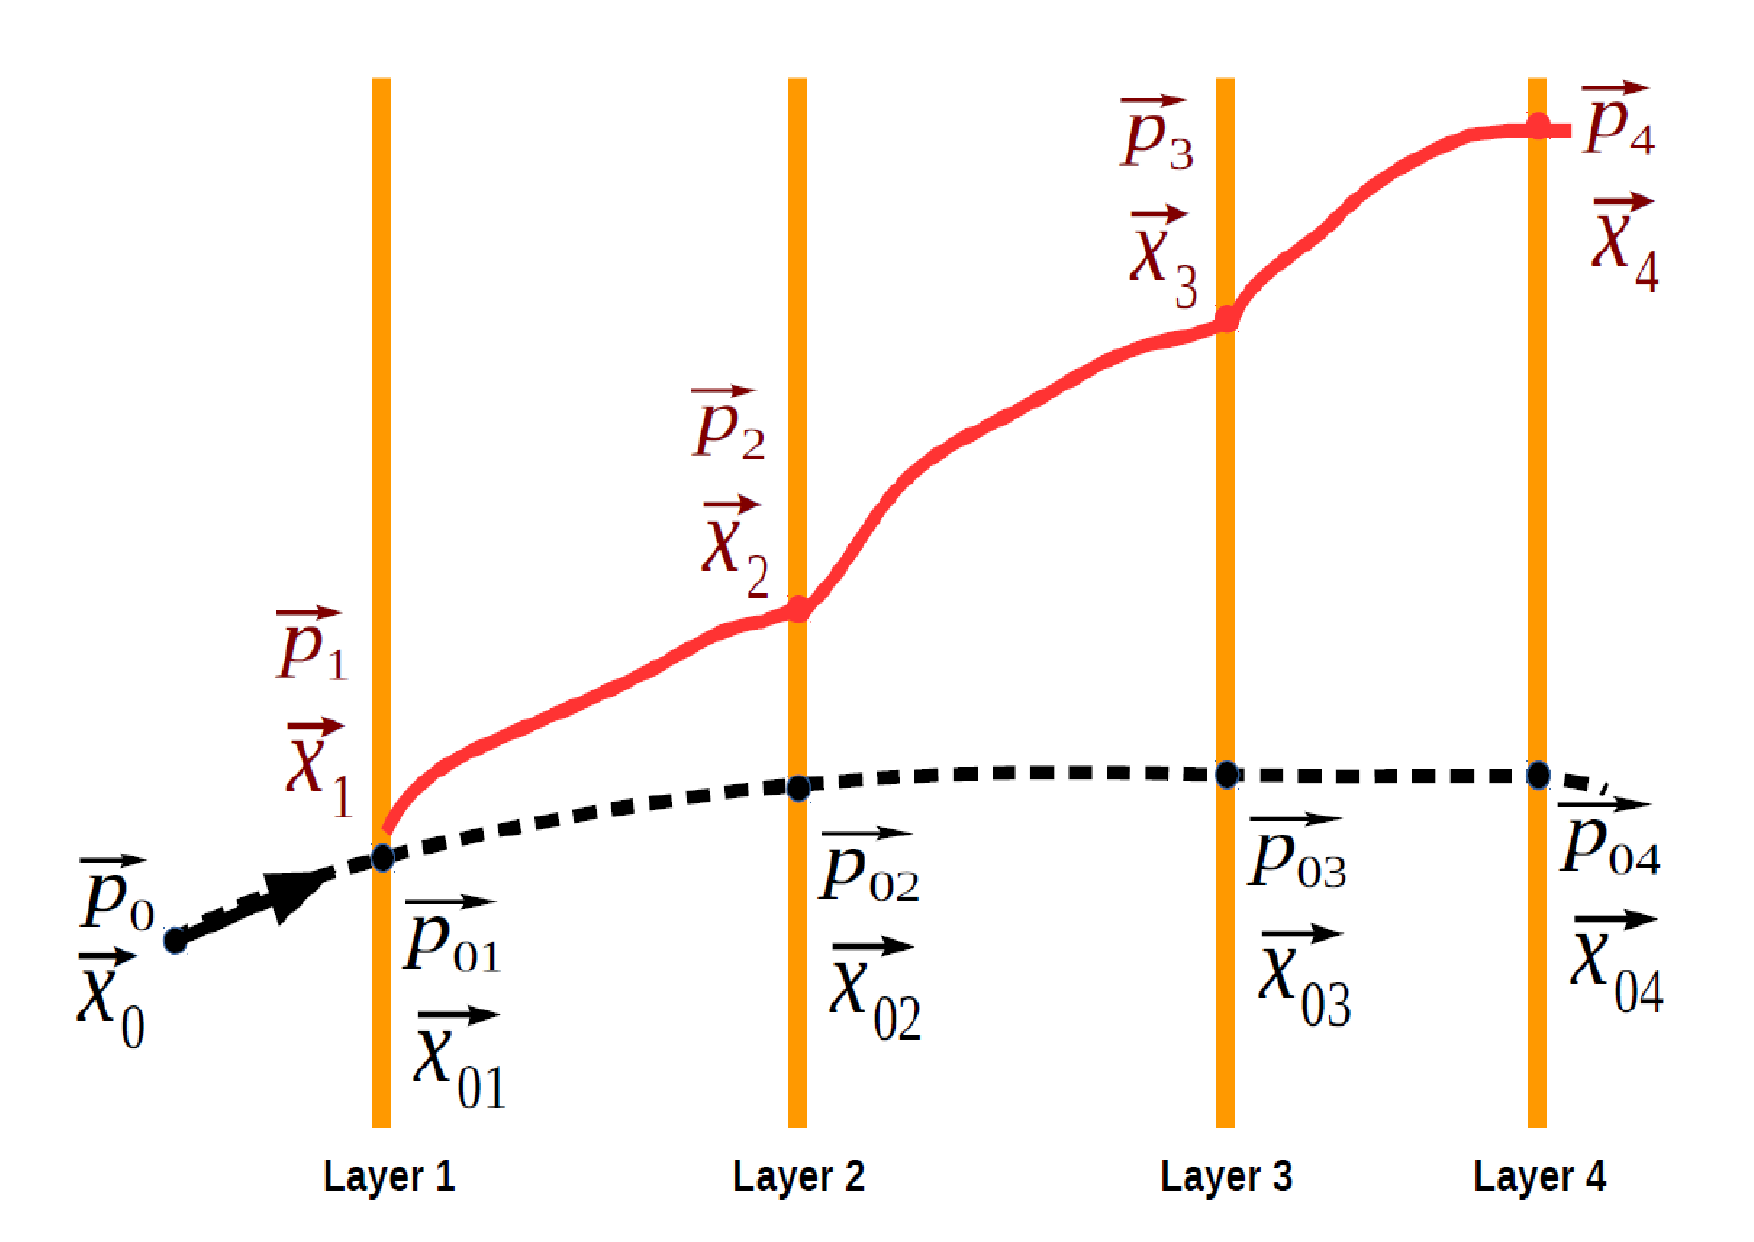
\includegraphics[width=0.7\textwidth]{figures/CalcSquem.pdf}
  \caption{Schematics for calculation of space point covariance matrix due to MS.}
  \label{fig:CalcSquem}
\end{figure}

The process begins with the calculation of the track average trajectory. This corresponds to trace the particle's trajectory 
ignoring MS and $E_{\rm loss}$ fluctuations, as these effects average out to zero. The trajectory will be the solution of the 
equation of motion within a magnetic field,

\begin{equation}
  \frac{d^2 \vec{r}}{ds^2} = \frac{q}{p}\frac{d\vec{r}}{ds}\times \vec{B},
\end{equation}
\noindent
where $q$ is the particles charge, $p$ is momentum magnitude which is constant, $\vec{B}$ the B-field and $s$ is the path-length along 
the trajectory. The solution of this equation for a given set of initial conditions, $\vec{x_0}$ and $\vec{p_0}$, can be written as,

\begin{equation}
  \vec{r} = \vec{f}(s;\vec{x}_0,\vec{p}_0).
\end{equation}
\noindent
The corresponding momentum along the trajectory is given by,
\begin{equation}
  \vec{p} = \vec{\kappa}(s;\vec{x}_0,\vec{p}_0) = p\frac{\partial \vec{f}(s;\vec{x}_0,\vec{p}_0)}{\partial s}.
\end{equation}

Lets suppose that the particle starts at the initial location $\vec{x_0}$ with momentum $\vec{p_0}$, and intersects a set of materials as 
shown in figure~\ref{fig:CalcSquem}. The black-dotted line shows the average trajectory. The red-solid line shows the actual trajectory
including the MS and $E_{\rm loss}$ fluctuations at the intersection with every material. The intersection coordinates and momenta, 
$\vec{x}_{0,i}$ and $\vec{p}_{0,i}$, of the average trajectory are given by

\begin{eqnarray}
  \vec{x}_{0,i} &=& \vec{f}(s_i;\vec{x_0},\vec{p_0})      = \vec{f}(s_i - s_{i-1};\vec{x}_{0,i-1},\vec{p}_{0,i-1}), \\
  \vec{p}_{0,i} &=& \vec{\kappa}(s_i;\vec{x_0},\vec{p_0}) = \vec{\kappa}(s_i - s_{i-1};\vec{x}_{0,i-1},\vec{p}_{0,i-1}).
\end{eqnarray}
\noindent

We start by considering the effects of MS. Lets denote the coordinates and momenta after intersecting the material of the actual particle trajectory by 
$\vec{x}_{i}$ and $\vec{p}_{i}$. At the intersection with layer-1 we have,

\begin{eqnarray}
  x^{k}_{1} &=& x^{k}_{0,1}, \\
  p^{k}_{1} &=& p^{k}_{0,1} + \delta p^{k}_{1};
\end{eqnarray}
\noindent
where $k=1,2,3$, and $\delta p^k_{1}$ is the effect of the multiple scattering at layer-1. This effect can be written as,

\begin{equation}
  \delta p^{k}_{1} = |\vec{p}_{01}|(\hat{m}^{k}_{11}\theta_{11} + \hat{m}^{k}_{12}\theta_{12}),
\end{equation}
\noindent
where $\hat{m}_{11}$ and $\hat{m}_{12}$ are any two mutually orthogonal unitary vector orthogonal to the momentum just 
previous to the intersection with the material; and $\theta_{11}$ and $\theta_{12}$ are the multiple scattering angles 
along the the $\hat{m}_{11}$ and $\hat{m}_{12}$ directions.

The coordinates and momenta of the actual trajectory just after layer-2 are given by,
\begin{eqnarray}
  \label{eq:x2}
  x^{k}_{2} &=& f^{k}(s_2 - s_1;\vec{x_1},\vec{p_1}) = f^{k}(s_2 - s_1;\vec{x}_{0,1},\vec{p}_{0,1} + \delta \vec{p}_{1}), \\
  p^{k}_{2} &=& \kappa^{k}(s_2 - s_1;\vec{x_1},\vec{p_1}) + \delta p^{k}_{2} = \kappa^{k}(s_2 - s_1;\vec{x}_{0,1},\vec{p}_{0,1} + \delta \vec{p}_{1}) + \delta p^{k}_{2};
\end{eqnarray}
\noindent
where
\begin{equation}
  \delta p^{k}_{2} = |\vec{p}_{02}|(\hat{m}^{k}_{21}\theta_{21} + \hat{m}^{k}_{22}\theta_{22}).
\end{equation}
\noindent
with $\hat{m}_{2i}$ and $\theta_{2i}$ a similar meaning as in the case of the intersection with layer-1.

\noindent
Equation~\ref{eq:x2} can be rewritten as,
\begin{eqnarray}
  x^{k}_{2} &=& f^{k}(s_2 - s_1;\vec{x}_{0,1},\vec{p}_{0,1})      + \frac{\partial f^{k}(s_2 - s_1;\vec{x}_{0,1},\vec{p}_{0,1})}{\partial p^{j}} \delta p^{j}_{1}      = x^{k}_{0,2} + \Delta x^{k}_{2}, \\
  p^{k}_{2} &=& \kappa^{k}(s_2 - s_1;\vec{x}_{0,1},\vec{p}_{0,1}) + \frac{\partial \kappa^{k}(s_2 - s_1;\vec{x}_{0,1},\vec{p}_{0,1})}{\partial p^{j}} \delta p^{j}_{1} + \delta p^{k}_{2} = p^{k}_{0,2} + \Delta p^{k}_{2};
\end{eqnarray}
\noindent
with
\begin{eqnarray}
  \label{eq:DelX2}
  \Delta x^{k}_{2} &=& {\mathcal F_{p}}^{kj}_{21} \delta p^{j}_{1}, \\
  \Delta p^{k}_{2} &=& {\mathcal K_{p}}^{kj}_{21} \delta p^{j}_{1}  + \delta p^{k}_{2};
\end{eqnarray}
\noindent
where the matrices ${\mathcal F_{p}}_{21}$ and ${\mathcal K_{p}}_{21}$ are given by
\begin{eqnarray}
  {\mathcal F_{p}}_{21} &=& \frac{\partial \vec{f}(s_2 - s_1;\vec{x}_{0,1},\vec{p}_{0,1})}{\partial \vec{p}}, \\
  {\mathcal K_{p}}_{21} &=& \frac{\partial \vec{\kappa}(s_2 - s_1;\vec{x}_{0,1},\vec{p}_{0,1})}{\partial \vec{p}}.
\end{eqnarray}

~\\
\noindent
In a similar fashion, the coordinates and momenta of the actual trajectory just after layer-3 are given by,
\begin{eqnarray}
  \label{eq:x3}
  x^{k}_{3} &=& f^{k}(s_3 - s_2;\vec{x_2},\vec{p_2}) = f^{k}(s_3 - s_2;\vec{x}_{0,2} + \Delta \vec{x}_{2},\vec{p}_{0,2} + \Delta \vec{p}_{2}), \\
  p^{k}_{3} &=& \kappa^{k}(s_3 - s_2;\vec{x_2},\vec{p_2}) + \delta p^{k}_{3} = \kappa^{k}(s_3 - s_2;\vec{x}_{0,1} + \Delta\vec{x}_{2},\vec{p}_{0,1} + \Delta \vec{p}_{2}) + \delta p^{k}_{3};
\end{eqnarray}
\noindent
with $\Delta \vec{x}_{2}$ and $\Delta \vec{p}_{2}$ given by Equation~\ref{eq:DelX2}, and $\delta p^{k}_{3}$ is the effect of MS after traversing the layer-3, with similar expression as in the 
previous cases. Again, Equation~\ref{eq:x3} can be rewritten as
\begin{eqnarray}
  x^{k}_{3} &=& x^{k}_{0,3}  + \frac{\partial f^{k}(s_3 - s_2;\vec{x}_{0,1},\vec{p}_{0,1})}{\partial x^{j}} \Delta x^{j}_{2} + \frac{\partial f^{k}(s_3 - s_2;\vec{x}_{0,1},\vec{p}_{0,1})}{\partial p^{j}} \Delta p^{j}_{2}, \\
  p^{k}_{3} &=& p^{k}_{0,2}  + \frac{\partial \kappa^{k}(s_3 - s_2;\vec{x}_{0,1},\vec{p}_{0,1})}{\partial x^{j}} \Delta x^{j}_{2} + \frac{\partial \kappa^{k}(s_3 - s_2;\vec{x}_{0,1},\vec{p}_{0,1})}{\partial p^{j}} \Delta p^{j}_{2} + \delta p^{k}_{2};
\end{eqnarray}
\noindent
which can be rewritten as
\begin{eqnarray}
  x^{k}_{3} &=& x^{k}_{0,3} + \Delta x^{k}_{2}, \\
  p^{k}_{3} &=& p^{k}_{0,3} + \Delta p^{k}_{2};
\end{eqnarray}
\noindent
with 
\begin{eqnarray}
  \label{eq:DelX3}
  \Delta x^{k}_{3} &=& {\mathcal F_{r}}^{kj}_{32} \Delta x^{j}_{2} + {\mathcal F_{p}}^{kj}_{32} \Delta p^{j}_{2}, \\
  \Delta p^{k}_{3} &=& {\mathcal K_{r}}^{kj}_{32} \Delta x^{j}_{2} + {\mathcal K_{p}}^{kj}_{32} \Delta p^{j}_{2}  + \delta p^{k}_{3};
\end{eqnarray}
\noindent
where the matrices ${\mathcal F_{r}}_{32}$, ${\mathcal F_{p}}_{32}$, ${\mathcal K_{r}}_{32}$ and ${\mathcal K_{p}}_{32}$ are given by
\begin{eqnarray}
  {\mathcal F_{r}}_{32} &=& \frac{\partial \vec{f}(s_3 - s_2;\vec{x}_{0,2},\vec{p}_{0,2})}{\partial \vec{x}}, \\
  {\mathcal F_{p}}_{32} &=& \frac{\partial \vec{f}(s_3 - s_2;\vec{x}_{0,2},\vec{p}_{0,2})}{\partial \vec{p}}, \\
  {\mathcal K_{r}}_{32} &=& \frac{\partial \vec{\kappa}(s_3 - s_2;\vec{x}_{0,2},\vec{p}_{0,2})}{\partial \vec{x}}, \\
  {\mathcal K_{p}}_{32} &=& \frac{\partial \vec{\kappa}(s_3 - s_2;\vec{x}_{0,2},\vec{p}_{0,2})}{\partial \vec{p}}.
\end{eqnarray}

~\\
\noindent
In general the $\Delta x^{k}_{n}$ and $\Delta p^{k}_{n}$ can be written as
\begin{eqnarray}
  \Delta x^{k}_{n} &=& \sum^{n-1}_{l = 1} F^{kj}_{n,l} \delta p^{j}_{l}, \\
  \Delta p^{k}_{n} &=& \sum^{n-1}_{l = 1} K^{kj}_{n,l} \delta p^{j}_{l} + \delta p^{j}_{n}.
\end{eqnarray}
\noindent
Where $\delta p^{j}_{l}$ is the MS effect just after layer-$l$ and given by,
\begin{equation}
  \delta p^{j}_{l} = |\vec{p}_{0l}|(\hat{m}^{j}_{1l}\theta_{1l} + \hat{m}^{j}_{1l}\theta_{1l}),
\end{equation}
\noindent
and where the $F^{kj}_{n,l}$ and $K^{kj}_{n,l}$ matrices are given by the recurrent formulas
\begin{equation}
  F^{kj}_{n,l} = \left\{
  \begin{array}{ll}
    {\mathcal F_{r}}^{km}_{n,n-1} F^{mj}_{n-1,l} + {\mathcal F_{p}}^{km}_{n,n-1} K^{mj}_{n-1,l} & \mbox{if } l < n-1 \\
    {\mathcal F_{p}}^{km}_{n,n-1}                                                               & \mbox{if } l = n-1
   \end{array}
  \right.
\end{equation}
\noindent
and 
\begin{equation}
  K^{kj}_{n,l} = \left\{
  \begin{array}{ll}
    {\mathcal K_{r}}^{km}_{n,n-1} F^{mj}_{n-1,l} + {\mathcal K_{p}}^{km}_{n,n-1} K^{mj}_{n-1,l} & \mbox{if } l < n-1 \\
    {\mathcal K_{p}}^{km}_{n,n-1}                                                               & \mbox{if } l = n-1
   \end{array}
  \right.
\end{equation}

\noindent
This allows to calculate the covariance matrix due to MS among the $\Delta x^{k}_{n}$ as follows
\begin{equation}
  \label{eq:Cov_X_MS_1}
  \left<  \Delta x^i_n x^j_m \right >_{\rm MS} = \sum^{n-1}_{l=1}\sum^{m-1}_{a=1} F^{ik}_{n,l} F^{jb}_{m,a} \left< \delta p^{k}_{l} \delta p^{b}_{a} \right>.
\end{equation}
\noindent
The covariance matrix among the $\delta p^k_l$ is given by
\begin{equation}
  \left< \delta p^{k}_{l} \delta p^{b}_{a} \right> = |\vec{p}_{0l}||\vec{p}_{0a}| (\hat{m}^k_{1l}\hat{m}^b_{1a} \left< \theta_{1l}\theta_{1a} \right> + \hat{m}^k_{1l}\hat{m}^b_{2a} \left< \theta_{1l}\theta_{2a} \right> + \hat{m}^k_{2l}\hat{m}^b_{1a} \left< \theta_{2l}\theta_{1a} \right> + \hat{m}^k_{2l}\hat{m}^b_{2a} \left< \theta_{2l}\theta_{2a} \right> )
\end{equation}
\noindent
The MS angles $\theta_{ik}$ are totally uncorrelated, {\it i.e.} $\left< \theta_{kl}\theta_{ma} \right> = \delta_{km}\delta_{la}(\theta^0_{l})^2$, with $\theta^0_{l}$ the mean-root-square 
of the MS angle at layer-$l$, which is given by the usual formula~\cite{bib:MS_angle},
\begin{equation}
  \theta^{0}_{l} = \frac{13.6~{\rm MeV/c}}{c\beta_{0,l}p_{0,l}} q \sqrt{x/X_0} \left[ 1 + 0.038 ln(x/X_0) \right],
\end{equation}
\noindent
where $q$, $p_{0,l}$, $c\beta_{0,l}$, are the charge number, momentum and velocity of the incident particle, and $x/X_0$ is the thickness of the scattering medium in radiation lengths.

Finally, $\left<  \Delta x^i_n x^j_m \right >_{\rm MS}$ can be written as follows,
\begin{equation}
  \left<  \Delta x^i_n x^j_m \right >_{\rm MS} = p^2 \sum^{n-1}_{l=1}\sum^{m-1}_{a=1} F^{ik}_{n,l} F^{jb}_{m,a} \left(\hat{m}^k_{1l}\hat{m}^b_{1a} + \hat{m}^k_{2l}\hat{m}^b_{2a}\right) \delta_{la} (\theta^0_l)^2,
\end{equation}
\noindent
where $p$ is the particle's momentum.


~\\
\noindent
A similar calculation can be used for the energy loss fluctuations. It is only needed to replace in eq.~\ref{eq:Cov_X_MS_1} the corresponding expression for the $\left< \delta p^{k}_{l} \delta p^{b}_{a} \right>$.
The $\delta p^{k}_{l}$ due to energy loss fluctuations can be written as,

\begin{equation}
  \delta p^{k}_{l} = \left(\frac{E}{p}\right) \hat{p}^{k}_{l} \sigma^{l}(E_{\rm loss}),
\end{equation}
\noindent
where $E/p$ is the particle's energy-momentum ratio, $\hat{p}^{k}_{l}$ is the $k$-component of the particle's momentum direction at intersection $l$, and 
$\sigma^{l}(E_{\rm loss})$ is the $E_{\rm loss}$ RMS at intersection $l$. For this last one we use a simple model proposed by the ALICE collaboration, 

\begin{equation}
  \label{eq:sigmaEloss}
  \sigma^{l}(E_{\rm loss}) = \kappa \times \sqrt{E^l_{\rm loss}},
\end{equation}
\noindent
where ${E^l_{\rm loss}}$ is calculated from the famous $dE/dx$ Bethe-Bloch formula~\cite{bib:MS_angle}, and $\kappa$ is a parameter which has been tuned to the value 0.015 
when the both $\sigma^{l}(E_{\rm loss})$ and $E^l_{\rm loss}$ are expressed in ${\rm GeV}$. The $\kappa$-tunning has being made by comparing the {\guari} output with the ILD 
full-simulation tracking performances. We can now calculate $\left< \delta p^{k}_{l} \delta p^{b}_{a} \right>$ due to the $E_{\rm loss}$ fluctuation,

\begin{equation}
  \left< \delta p^{k}_{l} \delta p^{b}_{a} \right> = \left( \frac{E}{p} \right)^2 \left(\hat{p}^{k}_{l}\hat{p}^{b}_{a}\right)\delta_{la}\sigma^{l}(E_{\rm loss}),
\end{equation}
\noindent
where the $\delta_{la}$ is due to the independence of the $E_{\rm loss}$ fluctuations at the different intersections.

Finally, $\left<  \Delta x^i_n x^j_m \right >_{E_{\rm loss}}$ can be written as follows,
\begin{equation}
  \left<  \Delta x^i_n x^j_m \right >_{E_{\rm loss}} = \left( \frac{E}{p} \right)^2 \sum^{n-1}_{l=1}\sum^{m-1}_{a=1} F^{ik}_{n,l} F^{jb}_{m,a} \left(\hat{p}^k_l\hat{p}^b_{a}\right) \delta_{la} \sigma^{l}(E_{\rm loss}).
\end{equation}


~\\
\noindent
In {\guari} package the measurement coordinates are expressed in terms of the sensor's local reference frame $\vec{x'}$, where the third coordinate is always perpendicular to the sensitive surface. 
The latest are functions of the global coordinates $\vec{x}$. The covariance matrix among the measurement coordinates in the sensor's local frame can be written as,

\begin{eqnarray}
  \left<  \Delta x'^i_n x'^j_m \right > &=& \delta_{ij}\delta_{nm}\sigma^i_n\sigma^j_m + \frac{\partial x'^i_n}{\partial x^k_n} \frac{\partial x'^j_m}{\partial x^r_m} \left( \left<  \Delta x^k_n x^r_m \right >_{\rm MS} + \left<  \Delta x^k_n x^r_m \right >_{E_{\rm loss}} \right) \\
                                        &=& V_{\rm sp} + V_{MS} + V_{E_{\rm loss}},
\end{eqnarray}
\noindent
where the first term describes the sensor's intrinsic resolution, the second the MS and the third the $E_{\rm loss}$ fluctuations.

~\\
Finally, the expression for the track parameters covariance matrix can be calculated as follows. Lets arrange the set of measurement coordinates in the array $\Gamma^{\rm meas}_i$, and lets 
$\Gamma_i(\vec{\alpha})$ be the track intersection coordinates with the different measurement layers as a function of the track parameters $\vec{\alpha}$. As an example, in the case of a straight 
line (helix) $\vec{\alpha}$ is a vector of size 4 (5). The track fitting consist at minimizing the $\chi^2$ given by

\begin{equation}
  \chi^2 = \sum_{i,j} (\Gamma_i(\vec{\alpha}) - \Gamma^{\rm meas}_i) \left(V\right)^{-1}_{ij} (\Gamma_j(\vec{\alpha}) - \Gamma^{\rm meas}_j),
\end{equation}
\noindent
where $V$ is the total covariance matrix $V = V_{\rm sp} + V_{MS} + V_{E_{\rm loss}}$. The track parameters covariance matrix is given by
\begin{equation}
 \left(V_{\vec{\alpha}} \right)^{-1}_{km} = \frac{1}{2}\frac{\partial^2\chi^2}{\partial \alpha_k \partial \alpha_m} = \sum_{i,j} \frac{\partial \Gamma_i(\vec{\alpha})}{\partial \alpha_k} \left(V \right)^{-1}_{ij} \frac{\partial \Gamma_j(\vec{\alpha})}{\partial \alpha_m}.
\end{equation}
\noindent
where the derivatives are evaluated at the actual known values of the track parameters, which can be easily calculated from the initial conditions $\vec{x}_0$ and $\vec{p}_0$ at the particle's origin.

\subsection{Tracking efficiency calculation}
\label{subsec:TrkEffic_calculation}

The tracking efficiency calculation depends on the track-finding algorithm used. For the time being only one such algorithm has been implemented and described in the next section.
Later in this document (c.f. sec.~\ref{subsec:track_finder_class}) some guide lines to implement a new pattern recognition algorithms will be given.

\subsubsection{FPCCD track finder}
\label{subsubsec:FPCCDTrkEffic_calculation}

This track finder is inspired in the FPCCD track-finder, one of the pattern recognition algorithms used by the ILD collaboration~\cite{bib:ILD_FPCCD_TrackFinder}, which
was developed to take advantage of fine pixel CCD silicon sensors. The tracking efficiency calculation that will be detailed here below uses the same features as the ALICE 
ITS Upgrade fast-simulation~\cite{bib:ALICE_fastsim}.

The procedure starts by calculating the efficiency ($P_{\rm seed}$) of so-called seeding configurations, which consist of sets of three layers for the reconstruction of a seed 
track. The set of seed configurations should be adapted to the application and has to be defined by the user. The seed track parameters covariance matrix is then calculated and 
used to obtain the track pointing resolution at the next sensitive layer. If previous to that an insensitive layer is intersected, the track parameters covariance matrix is updated 
including the MS and $E_{\rm loss}$ fluctuations of the insensitive layer. This track pointing resolution is then used to calculate the probability of good, fake or null track-hit 
association ($P_l$). If a hit is associated (either good or fake) the track parameters covariance matrix is updated adding this new measurement point. The extrapolation process is 
continued until no more sensitive layers are found.

The tracking efficiency of a given seed configuration with the corresponding configuration of associated good, fake and null hits is given by,

\begin{equation}
 \epsilon^k = P^k_{\rm seed} \prod_l P_l,
\end{equation}
\noindent
where $P^k_{\rm seed}$ is the efficiency for the seeding configuration $k$ and $P_l$ is the probability of either good, fake or null track-hit association at layer $l$. This equation 
ignores possible correlations among the seeding efficiency and the track-hit associations of the subsequent layers.

The total tracking efficiency is given by
\begin{equation}
 \epsilon = \sum_k \epsilon^k,
\end{equation}
\noindent
where the sum runs over all the seeding configurations plus associated hits respecting some constrains such as: minimum number of hits in the track, minimum purity 
(\# good hit association)/(\# total hits), ...

Each configuration $k$ will have as well its own track parameters covariance matrix $V^k_{\vec{\alpha}}$. The average covariance matrix will be give by,

\begin{equation}
 \left< V_{\vec{\alpha}} \right>  = \frac{\sum_k \epsilon^k V^k_{\vec{\alpha}} } { \sum_k \epsilon^k }.
\end{equation}
\noindent
The output of the whole calculation will then be the tracking efficiency as well as the average track parameters covariance matrix.

~\\
\noindent
In the following sub-sections are detailed the calculations for the seeding configuration efficiency and the track-hit association probabilities.

\subsubsection*{Seeding probability calculation}

As mentioned above, the seeding configurations are a list of combinations of three layers used to reconstruct a seed track. The actual combinations are application 
dependent and should then be specified by the user. In the process of pattern recognition in a real experiment the list of seed configurations will be hierarchized, 
starting by the most likely one. In a collider experiment with a tracker with cylindrical symmetry with respect to the beam lines the seeding should start with 
combinations of the outermost layers, the ones with the lower hit rates density (hit per unit of time per unit of surface), as this reduces the amount of combinatorics.
If some of the track hits on the outermost layers go undetected the corresponding seeding configuration will not be found. In order to increase tracking efficiency 
some other combinations with inner layers could also be tested but at the expense of increased combinatorics.

The seeding efficiency is modeled as the product of three components,

\begin{equation}
 P_{\rm seed} = P({\rm intrinsic}) P(p^{\rm min}_t) P(\chi^2/ndf~cut),
\end{equation}
\noindent
where $P({\rm intrinsic})$ is the intrinsic probability of the seeding configuration, $P(p^{\rm min}_t)$ the probability for the seed configuration to pass a 
minimum $p^{\rm min}_t$ cut, and $P(\chi^2/ndf~cut)$ the probability of the seed track to pass a maximum $\chi^2/ndf$ cut.

$P(\chi^2/ndf~cut)$ is easily calculated as the probability for a $\chi^2$ distribution with $ndf$ degrees of freedom to be smaller than a certain maximum $(\chi^2/ndf)_{\rm max}$ 
specified by the user. The $ndf$ is calculated as the difference $ndf = 2n_{\rm hits} - n_{\rm trk-params}$, where $n_{\rm hits}$ is the number of hits to reconstruct 
the seed track (in this case three) and $n_{\rm trk-params}$ is the number of track parameters (in this case five).

$P({\rm intrinsic})$ depends on the number of good, fake and null hits related with the seed configuration. This will be easier to understand by considering an example. 
Lets consider a track that intersects the four outermost layers of a tracker, denoted by $l_1$, $l_2$, $l_3$, $l_4$, respectively. The following set of seed configurations 
could be specified,

\begin{itemize}
 \item  $(l_2,l_3,l_4)$,
 \item  $(l_1,l_3,l_4)$,
 \item  $(l_1,l_2,l_4)$,
 \item  $(l_1,l_2,l_3)$.
\end{itemize}
\noindent
The first configuration $(l_2,l_3,l_4)$ corresponds to a seed track with hits on the 3 outermost layers. The intrinsic probability for this configuration is given by 
$P^2_{\rm hit} P^3_{\rm hit} P^4_{\rm hit}$, where $P^k_{\rm hit}$ is the probability of having either a good or fake hit at layer $k$. The second
configuration $(l_1,l_3,l_4)$ means that no hit was found at layer $2$, so the intrinsic probability is given by $P^1_{\rm hit} P^2_{\rm null} P^3_{\rm hit} P^4_{\rm hit}$, 
where $P^2_{\rm null}$ is the probability of not finding a hit on layer 2. The other seed configurations will have similar expressions.

The probability for finding a good hit in the seed layer $k$ ($P^k_{\rm good}$) is simply the layer intrinsic detection efficiency $P^k_{\rm good} = \epsilon^k_{\rm det}$. 
The probability for no hit in the seed layer $k$ ($P^k_{\rm null}$) is given by the product of not detecting the real track hit ($1 - \epsilon^k_{\rm det}$) and 
not finding a fake hit ($P^k_{\rm no-fake}$),

\begin{equation}
 P^k_{\rm null} = (1 - \epsilon^k_{\rm det}) P^k_{\rm no-fake}.
\end{equation}
\noindent
$P^k_{\rm no-fake}$ is calculated by using the layer hit rate $R^k_{\rm bkg}$, read-out time $t^k_{\rm r.o.}$ and a surface $S^k$. The average number of fake hit 
will be given by $N^k_{\rm bkg} = R^k_{\rm bkg} t^k_{\rm r.o.} S^k$. Assuming that the number of fake hits are Poisson distributed, $P^k_{\rm no-fake}$ is 
given by,

\begin{equation}
  P^k_{\rm no-fake} = Poisson(0,N^k_{\rm bkg}) = e^{-N^k_{\rm bkg}}.
\end{equation}
\noindent
The last element to define is the surface $S^k$. This is given by the size of the region where the real track hits have a sizable probability. This is given by the 
surface of the $1-\sigma$ ellipse ($S^k_{1\sigma}$), which includes the sensor intrinsic resolution, MS and $E_{\rm loss}$ fluctuations, multiplied the a factor related 
to the $(\chi^2/ndf)_{\rm max}$ on the seed track,

\begin{equation}
  S^k = \left[(\chi^2/ndf)_{\rm max}\right]^{1/2} S^k_{1\sigma}.
\end{equation}
\noindent
The probability of finding a fake hit at the seed layer $k$ ($P^k_{\rm fake}$) is given by,

\begin{equation}
  P^k_{\rm fake} = 1 - P^k_{\rm good} - P^k_{\rm null} = (1 - \epsilon^k_{\rm det}) (1 - P^k_{\rm no-fake}).
\end{equation}

~\\
\noindent
The Last component of the seeding efficiency to discuss is the term related to the $p^{\rm min}_t$ cut, $P(p^{\rm min}_t)$. This term is characteristic of the FPCCD pattern 
recognition algorithm, which track seeding process is illustrated in figure~\ref{fig:FPCCD_Seeding}. This algorithm looks for a hit in the outermost seed layer of a given 
seeding configuration. If a hit is found then it proceeds to draw on the plane perpendicular to the uniform magnetic field two hypothetical tracks generated at the center-point, 
going through the hit on the outer layer, having $p_t = p^{\rm min}_t$ and having a $\pm1$ electric charge. This defines a search window for looking for hits in the other inner seed 
layers. If hits are found within this search window, then the track is fit and a $(\chi^2/ndf)_{\rm max}$ cut is applied. This is how a $p^{\rm min}_t$ cut is applied on the seed 
tracks. The efficiency due to this $p^{\rm min}_t$ cut should be 0 (1) for tracks with $p_t$ much below (above) $p^{\rm min}_t$, and should show a quick $0 \rightarrow 1$ transition 
for $p_t$ around $p^{\rm min}_t$.

\begin{figure}
  \centering
  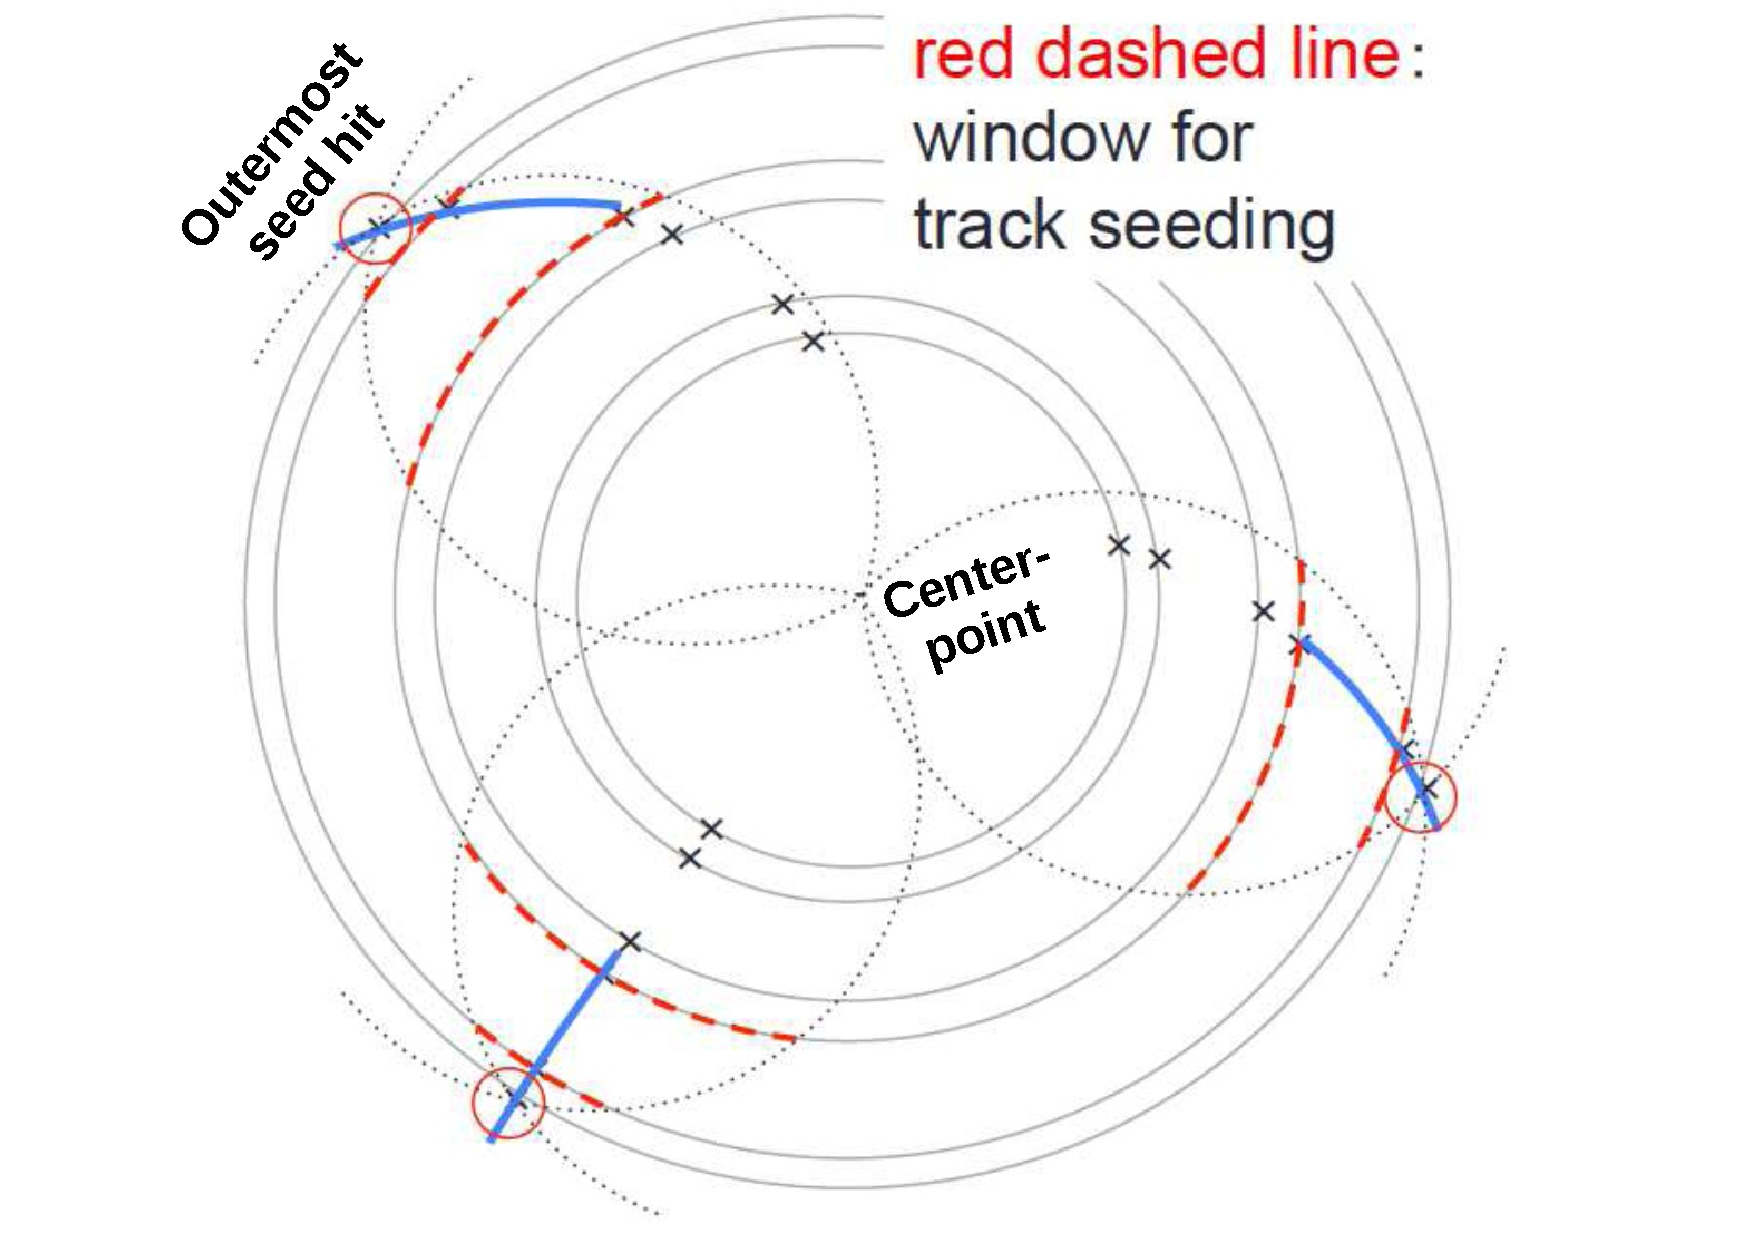
\includegraphics[width=0.6\textwidth]{figures/FPCCD_Seeding.pdf}
  \caption{Graphical representation of track seeding process for the FPCCD track-finder algorithm. Crosses denote hits on the tracker. 
  Crosses surrounded by red circles in the outer layer are used to determine a wide enough search region to catch track seeds with $p_t > p^{\rm min}_t$. 
  Dotted curved lines denote tracks passing through the outermost seed hit, through a center-point and with $p_t = p^{\rm min}_t$. Red dashed lines 
  denote search windows for generating track seeds, and their length is determined by intersections between layers and the dotted curved lines. Blue 
  curved lines denote the track seeds generated by this process.}
  \label{fig:FPCCD_Seeding}
\end{figure}

In this package this $p^{\rm min}_t$ cut seed efficiency is calculated with a MC method. For this the three seed hits are sampled $N_{\rm sampling}$ times with a multi-variate 
Gaussian distribution with the their actual covariance matrix. For each sampling, the outermost seed hit is used to define the search window as described above. It is then 
count the amount of samplings ($N_{\rm passed}$) in which the two innermost seed hits were found inside such search window. The efficiency is then simply defined as,

\begin{equation}
 P(p^{\rm min}_t) = \frac{N_{\rm passed}}{N_{\rm sampling}}.
\end{equation}
\noindent
For this calculation $N_{\rm sampling}$ should be defined by the user by finding a trade-off between precision and calculation time.

\subsubsection*{Track-hit association probabilities}

The track-hit association probability at a layer $l$ depends on the track pointing resolution onto the layer, the layer intrinsic resolution and the hit rate at this layer. 
The hit rate depends on many factors and tries to include effects such as sensor electric noise, event multiplicity, background and possible pile-up.

One can show that the probability that the correct cluster will be associated to extrapolated seed with smaller $\chi^2$ than any random hits can be expressed as 
(assuming infinite size search-window),

\begin{equation}
 P^{l}_{\rm corr} = \frac{\epsilon^l_{\rm det}}{1 + N^l_{\rm bkg}},
\end{equation}
\noindent
where $\epsilon^l_{\rm det}$ is the layer intrinsic detection efficiency and $N^l_{\rm bkg}$ is the expected number of fake hits within the region $S^l$ defined 
by the convolution of the track pointing resolution and the layer intrinsic resolution, {\it i.e.} $N^l_{\rm bkg} = R^l_{\rm bkg} t^l_{\rm r.o.} S^l$.
The above can be extended to use search windows of finite size. The correct track-hit association probability is then transformed to,

\begin{equation}
  P^{l}_{\rm corr} = \frac{\epsilon^{l}_{\rm det} \left( 1 - \gamma^{1 + N^l_{\rm bkg}} \right)}{1 + N^l_{\rm bkg}},
\end{equation}
\noindent
where $\gamma$ is the fraction of correct hits lost to the $\chi^2$ cut in the track-hit association process ({\it e.g.} $\gamma \simeq 5\%$ with $\chi^2/ndf < 3$ cut). 
The probability of no track-hit association is then,

\begin{equation}
  P^{l}_{\rm null} = \left(1 - \epsilon^l_{\rm det} + \epsilon^l_{\rm det}\gamma \right)  \gamma^{N^l_{\rm bkg}},
\end{equation}
\noindent
and finally, the probability to have a fake associated to the track is,
\begin{equation}
  P^{l}_{\rm fake} = 1 - P^l_{\rm corr} - P^l_{\rm null}.
\end{equation}


Therefore, three states (correct, fake and no association) are possible per layer. The number of possible outcomes also depends on the number of layers and is therefore $K_p =3^N$. 
Only one outcome corresponds to the simplified picture of correct cluster association on each single layer ($N$ correct track-hit associations). By adding the probabilities of {\it e.g.} 
having $N - 1$ correct associations and no association at the remaining layer would correspond to "correct tracks with at least $N - 1$ clusters" and so on.




\section{Geometry configuration}
\label{sec:GeoConf}

In this section are described the different elements for a geometry configuration as well as 
the syntax for the specification of the world volume, magnetic field, different geometry elements, 
resolution model, efficiency model, and systems and Telescope-DUT configurations.

In {\guari} there is an internal unit system. All physical quantities have to be specified with the corresponding units, 
otherwise the program will crash with an error message.

The volumes in space are placed by specifying a position and a set of three rotation angles $(\alpha_x,\alpha_y,\alpha_z)$ to 
determine its orientation. The rotation convention is 

\begin{equation}
  R = R_z(\alpha_x) R_z(\alpha_y) R_z(\alpha_z) 
\end{equation}
\noindent
where $R$ is the full rotation matrix, and $R_i(\alpha_i)$ are rotation matrices along the axis-$i$ by an angle $\alpha_i$. 
The rotation order if along the z-axis first, then along the y-axis and finally along the x-axis. The specification of the 
rotation angles is not mandatory, if not specified they will all be set to its default value $(0,0,0)$.


\subsection{World volume}

The world volume should contain all the geometry elements, and only inside it the track navigation will 
be performed. Currently, only two kinds of world volumes are possible, either a box or a cylinder. The specification 
is as follows,

\subsubsection{Box world volume}

The box world volume is specified as follows,
~\\
~\\
\noindent
{\tt BeginBoxWorldVolume} \\
$~~~~~${\tt Position   x   y   z  units   // (Mandatory)} \\
$~~~~~${\tt widthX     value  units  $~$  // (Mandatory, value > 0)} \\
$~~~~~${\tt widthY     value  units  $~$  // (Mandatory, value > 0)} \\
$~~~~~${\tt widthZ     value  units  $~$  // (Mandatory, value > 0)} \\
{\tt EndBoxWorldVolume} \\

\noindent
where {\tt Position} specifies the center of the box, and {\tt widthX,Y,Z} the widths along the global frame axes.

\subsubsection{Cylinder world volume}

The cylinder world volume is specified as follows,

\noindent
{\tt BeginCylinderWorldVolume} \\
$~~~~~${\tt Position   x   y   z  units  // (Mandatory)} \\
$~~~~~${\tt Radius     value  units  $~$ // (Mandatory, value > 0)} \\
$~~~~~${\tt Length     value  units  $~$ // (Mandatory, value > 0)} \\
{\tt EndCylinderWorldVolume} \\

\noindent
where {\tt Position} specifies the center of the cylinder. The other parameters are evident. The cylinder is always oriented along the 
global z-axis.

\subsection{Magnetic field}

Each geometry has its own magnetic field. If not specified it is assumed to be zero. Two types of B-field 
are currently implemented.

\subsubsection{Constant Magnetic field}

A constant B-field is build by specifying its magnitude and direction as shown below.
~\\
~\\
\noindent
{\tt BeginConstantBfield} \\
$~~~~~${\tt Magnitude    value  units      // (Mandatory, value > 0)} \\
$~~~~~${\tt Direction    x  y  z   $~~~~~$ // (Mandatory, vector will be normalized to unity)} \\
{\tt EndConstantBfield}

\subsubsection{Piece-wise Magnetic field}

This magnetic field consist of a set of non-overlapping volumes with a constant B-field inside each of them. If any pair of the 
specified volumes overlap, the program will crash with an error message. Outside all the volumes the B-field is zero by default, 
but it can be set to a non-zero values if specified. A set of volumes of different types can be specified. A set of so-called 
"inside-fields" have to be specified as well. The number of volumes have to match the number of inside-fields, otherwise the 
program will crash with an error message. The syntax for specifying this kind of B-field is as follows.

~\\
~\\
\noindent
{\tt BeginMultipleStepsBfield} \\
$~~~~~${\tt BeginSomeTypeVolume} \\
$~~~~~~~${...} \\
$~~~~~${\tt EndSomeTypeVolume}   \\
$~~~~~${\tt BeginInsideBfield} \\
$~~~~~~~${\tt Magnitude    value  units      // (Mandatory, value > 0)} \\
$~~~~~~~${\tt Direction    x  y  z   $~~~~~$ // (Mandatory, vector will be normalized to unity)} \\
$~~~~~${\tt EndInsideBfield} \\
$~~~~~${\tt ...} \\
$~~~~~${\tt BeginOutsideBfield} \\
$~~~~~~~${\tt Magnitude    value  units      // (Mandatory, value > 0)} \\
$~~~~~~~${\tt Direction    x  y  z   $~~~~~$ // (Mandatory, vector will be normalized to unity)} \\
$~~~~~${\tt EndOutsideBfield} \\
{\tt EndMultipleStepsBfield}

~\\
\noindent
The data structure inside {\tt BeginOutsideBfield} and {\tt EndOutsideBfield} is optional. If not specified 
then the "outside-field" will be set to zero. 

The {\tt SomeType} on {\tt BeginSomeTypeVolume} and {\tt EndSomeTypeVolume} represents the different types of 
volumes which can be specified, each of them with their own syntax. There are several volume types which are mentioned 
here below.

\begin{itemize}
  \item  {\bf Box volume}: specified as follows,

  \noindent
  {\tt BeginBoxVolume} \\
  $~~~~~${\tt Position   x  y  z  units                       $~~~$ // (Mandatory)} \\
  $~~~~~${\tt RotAngles  $\alpha_x$  $\alpha_x$  $\alpha_x$  units  // (Optional)} \\
  $~~~~~${\tt widthX     value   units                      $~~~~~$ // (Mandatory, value > 0)} \\
  $~~~~~${\tt widthY     value   units                      $~~~~~$ // (Mandatory, value > 0)} \\
  $~~~~~${\tt widthZ     value   units                      $~~~~~$ // (Mandatory, value > 0)} \\
  {\tt EndBoxVolume}
  
  \item {\bf Cylinder volume}: specified as follows,
  
  \noindent
  {\tt BeginCylinderVolume} \\
  $~~~~~${\tt Position   x  y  z  units                       $~~~$ // (Mandatory)} \\
  $~~~~~${\tt RotAngles  $\alpha_x$  $\alpha_x$  $\alpha_x$  units  // (Optional)} \\
  $~~~~~${\tt Radius     value   units                      $~~~~~$ // (Mandatory, value > 0)} \\
  $~~~~~${\tt Length     value   units                      $~~~~~$ // (Mandatory, value > 0)} \\
  {\tt EndCylinderVolume}
  
  \item {\bf Cone volume}: specified as follows,
  
  \noindent
  {\tt BeginConeVolume} \\
  $~~~~~${\tt Position   x  y  z  units                       $~~~$ // (Mandatory)} \\
  $~~~~~${\tt RotAngles  $\alpha_x$  $\alpha_x$  $\alpha_x$  units  // (Optional)} \\
  $~~~~~${\tt Radius1    value   units                       $~~~~$ // (Mandatory, value > 0)} \\
  $~~~~~${\tt Radius2    value   units                       $~~~~$ // (Mandatory, value > 0)} \\
  $~~~~~${\tt Length     value   units                      $~~~~~$ // (Mandatory, value > 0)} \\
  {\tt EndConeVolume}
  
  \item {\bf Disk section volume}: specified as follows,
  
  \noindent
  {\tt BeginDiskSectionVolume} \\
  $~~~~~${\tt Position   x  y  z  units                       $~~~$ // (Mandatory)} \\
  $~~~~~${\tt RotAngles  $\alpha_x$  $\alpha_x$  $\alpha_x$  units  // (Optional)} \\
  $~~~~~${\tt Rin        value   units                   $~~~~~~~~$ // (Mandatory, value > 0)} \\
  $~~~~~${\tt Rout       value   units                    $~~~~~~~$ // (Mandatory, value > 0)} \\
  $~~~~~${\tt Length     value   units                      $~~~~~$ // (Mandatory, value > 0)} \\
  $~~~~~${\tt DeltaPhi   value   units                        $~~~$ // (Mandatory, value > 0)} \\
  {\tt EndDiskSectionVolume}
  
  \noindent
  The disk section will expand an angle {\tt DeltaPhi} around the local x-axis.
  
  \item {\bf Cone section volume}: specified as follows,
  
  \noindent
  {\tt BeginConeSectionVolume} \\
  $~~~~~${\tt Position   x  y  z  units                       $~~~$ // (Mandatory)} \\
  $~~~~~${\tt RotAngles  $\alpha_x$  $\alpha_x$  $\alpha_x$  units  // (Optional)} \\
  $~~~~~${\tt Radius1    value   units                       $~~~~$ // (Mandatory, value > 0)} \\
  $~~~~~${\tt Radius2    value   units                       $~~~~$ // (Mandatory, value > 0)} \\
  $~~~~~${\tt Length     value   units                      $~~~~~$ // (Mandatory, value > 0)} \\
  $~~~~~${\tt DeltaPhi   value   units                        $~~~$ // (Mandatory, value > 0)} \\
  {\tt EndConeSectionVolume}
  
  \noindent
  The cone section will expand an angle {\tt DeltaPhi} around the local x-axis.
  
\end{itemize}


As an example, here below there is an example of a piece-wise B-field with two cylindric volumes along the z-axis with fields pointing 
in opposite directions, both along the x-axis.

~\\
\noindent
{\tt BeginMultipleStepsBfield} \\
$~~~~~${\tt BeginCylinderVolume} \\
$~~~~~~~${\tt Position   0.0 0.0 0.0 cm} \\
$~~~~~~~${\tt RotAngles  0.0 0.0 0.0 deg} \\
$~~~~~~~${\tt Radius     5.0  cm} \\
$~~~~~~~${\tt Length     2.0  cm} \\
$~~~~~${\tt EndCylinderVolume} \\
$~~~~~${\tt BeginInsideBfield} \\
$~~~~~~~${\tt Magnitude    1.0 T} \\
$~~~~~~~${\tt Direction    1 0 0} \\
$~~~~~${\tt EndInsideBfield} \\
$~~~~~${\tt BeginCylinderVolume} \\
$~~~~~~~${\tt Position   0.0 0.0 10.0 cm} \\
$~~~~~~~${\tt RotAngles  0.0 0.0  0.0 deg} \\
$~~~~~~~${\tt Radius     5.0  cm} \\
$~~~~~~~${\tt Length     2.0  cm} \\
$~~~~~${\tt EndCylinderVolume} \\
$~~~~~${\tt BeginInsideBfield} \\
$~~~~~~~${\tt Magnitude    1.0 T} \\
$~~~~~~~${\tt Direction   -1 0 0} \\
$~~~~~${\tt EndInsideBfield} \\
$~~~~~${\tt BeginOutsideBfield} \\
$~~~~~~~${\tt Magnitude    0.5 T} \\
$~~~~~~~${\tt Direction    0 1 0} \\
$~~~~~${\tt EndOutsideBfield} \\
{\tt EndMultipleStepsBfield}

\subsection{Simple geometries}

In this section will be described the syntax for the geometrical volumes up to now implemented in {\guari}. 
A complex geometry will be build using the simple geometrical volumes described in the sections below. In the 
specification of a geometry element a set of parameters are always mandatory, those which allow to place the 
volume on space and to assign its material properties. These volumes could be sensitive, {\it i.e.} detector, 
depending on the value of the bool variable {\tt IsSensitive}. In case it is set to {\tt true}, then the specification 
of additional parameters becomes mandatory. Those parameters refers to the detection performances of the sensitive 
element, such as intrinsic resolution ({\tt ResolutionU/V}), detection efficiency ({\tt Efficiency}), readout time 
({\tt ROtime}) and insensitive borders ({\tt InsensFracU/Vneg} and {\tt InsensFracU/Vpos}). The amount of hit rate 
({\tt BkgRate}, hits per unit of time and unit of surface) can also be specified. It is mainly used in the calculation 
of the tracking efficiency.

~\\
Lets now describe the syntax of the different geometrical volumes. The meaning of some parameters common to all
volumes will be fully described in the section~\ref{subsubsec:Plane}.

\subsubsection{Plane}
\label{subsubsec:Plane}

A so-called {\tt GeoPlane}, is a box in which one of its dimensions is much smaller than the other two. Its 
syntax is as follows,

~\\
\noindent
{\tt BeginGeoPlane} \\
$~~~~~${\tt Name             string                   $~~~~~~~~~~~~$   // (Mandatory)} \\
$~~~~~${\tt Position         x  y  z units                     $~~~$   // (Mandatory)} \\
$~~~~~${\tt RotAngles        $\alpha_x$  $\alpha_y$  $\alpha_z$ units  // (Optional)}  \\
$~~~~~${\tt Thickness        value  units                       $~~$   // (Mandatory, value > 0)} \\
$~~~~~${\tt Material         string                       $~~~~~~~~$   // (Mandatory)} \\
$~~~~~${\tt XOX0             value                   $~~~~~~~~~~~~~$   // (Optional)}  \\
$~~~~~${\tt widthU           value units                     $~~~~~$   // (Mandatory, value > 0)} \\
$~~~~~${\tt widthV           value units                     $~~~~~$   // (Mandatory, value > 0)} \\
$~~~~~${\tt IsSensitive      bool                          $~~~~~~~$   // (Mandatory)} \\
$~~~~~${\tt ResolutionU      value units                               // (Optional, value > 0)} \\
$~~~~~${\tt ResolutionV      value units                               // (Optional, value > 0)} \\
$~~~~~${\tt Resolution       value units                               // (Optional, value > 0)} \\
$~~~~~${\tt ROtime           value units                      $~~~~$   // (Optional, value > 0)} \\
$~~~~~${\tt Efficiency       value                          $~~~~~~$   // (Optional, 0 <= value <= 1)} \\
$~~~~~${\tt InsensFracUneg   value                              $~~$   // (Optional, default is zero)} \\
$~~~~~${\tt InsensFracUpos   value                              $~~$   // (Optional, default is zero)} \\
$~~~~~${\tt InsensFracVneg   value                              $~~$   // (Optional, default is zero)} \\
$~~~~~${\tt InsensFracVpos   value                              $~~$   // (Optional, default is zero)} \\
$~~~~~${\tt BkgRate          value units                       $~~~$   // (Optional, default is zero)} \\
$~~~~~${\tt SystemName       string                          $~~~~~$   // (Optional)} \\
$~~~~~${\tt LayerName        string                         $~~~~~~$   // (Optional)} \\
$~~~~~${\tt ResolutionModel  string                                    // (Optional)} \\
$~~~~~${\tt EfficiencyModel  string                                    // (Optional)} \\
{\tt EndGeoPlane}

~\\
The material budget in units of radiation lengths seen by a particle traversing some path $x$ the volume is calculated using the {\tt Material} 
name. {\guari} has a table of materials with their corresponding $X_0$. The material budget in then simply $x/X_0$. The material budget of a 
given element at normal incidence can be set by hand with the parameter {\tt XOX0}. If it is set, then the material budget at normal incidence, 
{\it i.e.} for a traversed path equal to the thickness, becomes {\tt XOX0}, and the material budget of an arbitrary path $x$ becomes 
$x/X_0 = (x/{\rm Thickness})\times${\tt XOX0}. This feature is useful when to model the material budget of a complicated composite of 
materials like a ladder with sensors, where several material are used to build the object: sensors, cables, supports, ... With this feature a 
single value of {\tt XOX0} has to be specified. This same feature is shared by all the other geometrical volumes.

The variables $U$ and $V$ above refer to the local coordinates on the so-called "main-surface" of the volume. It is 
a plane in the middle of the volume which is used as reference for the local reference frame. In the case of the 
{\tt GeoPlane} object, the main surface is a plane in the middle of the thickness, located at {\tt Position} with the 
{\tt RotAngles} orientation, and with widths {\tt widthU} and {\tt widthV}.

If the {\tt IsSensitive} parameter is set to {\tt true} the intrinsic resolutions along the local $U$ and $V$ directions 
has to be specified. They can be specified separately with the {\tt ResolutionU} and {\tt ResolutionV} parameters, or if 
they are the same it is only needed to specify the {\tt Resolution} parameter ({\tt ResolutionU/V = Resolution}).

The {\tt InsensFracUneg} and {\tt InsensFracUpos} only count for the case of {\tt IsSensitive} set to {\tt true}. These can be used to specify 
an insensitive length at the borders of the {\tt GeoPlane}. These parameters are fractions, {\it i.e.} the values they can have are inside
$[0,1]$, and their sum cannot exceed 1. The insensitive length at the low-edge (high-edge) along the local $U$ coordinate is calculated as 
{\tt InsensFracUneg}$\times${\tt widthU} ({\tt InsensFracUpos}$\times${\tt widthU}). So, even if a particle traverses the volume it can do it 
in a non-sensitive region. In such a case this intersection contributes with no measurement but only with material budget.
The parameters {\tt InsensFraVcneg} and {\tt InsensFracVpos} have a similar meaning.

The {\tt SystemName} and {\tt LayerName} parameters are optional. See the examples in section~\ref{subsec:Some_examples} for 
the usage of these parameters.

The {\tt ResolutionModel} parameter is a string referring to the name of an {\tt GResolutionModel} object. This object calculates 
the sensitive element spatial resolution of the measured point as a function of the intrinsic resolutions ({\tt ResolutionU/V}), 
the intersection coordinates and momentum of the particle with the main surface, and some other parameters. Its default value is an 
empty string, in such case the measurement spatial resolution is equal to the intrinsic resolution. See the example in 
section~\ref{subsubsec:Example3} for an illustration on how it can be used.

Finally, the {\tt EfficiencyModel} parameter is a string referring to the name of an {\tt GEfficiencyModel} object. This object 
calculates the sensitive element detection efficiency of the measured point point as a function of the intrinsic detection efficiency 
({\tt Efficiency}), the intersection coordinates and momentum of the particle with the main surface, and some other parameters. Its default 
value is an empty string, in such case the measurement detection efficiency is equal to the intrinsic detection efficiency.

\subsubsection{Cylinder}
\label{subsubsec:Cylinder}

A so-called {\tt GeoCylinder}, is a cylinder with a small radial thickness. Its syntax is as follows,

~\\
\noindent
{\tt BeginGeoCylinder} \\
$~~~~~${\tt Name             string                   $~~~~~~~~~~~~$   // (Mandatory)} \\
$~~~~~${\tt Position         x  y  z units                     $~~~$   // (Mandatory)} \\
$~~~~~${\tt RotAngles        $\alpha_x$  $\alpha_y$  $\alpha_z$ units  // (Optional)}  \\
$~~~~~${\tt Thickness        value  units                       $~~$   // (Mandatory, value > 0)} \\
$~~~~~${\tt Material         string                       $~~~~~~~~$   // (Mandatory)} \\
$~~~~~${\tt XOX0             value                   $~~~~~~~~~~~~~$   // (Optional)}  \\
$~~~~~${\tt Radius           value units                     $~~~~~$   // (Mandatory, value > 0)} \\
$~~~~~${\tt Length           value units                     $~~~~~$   // (Mandatory, value > 0)} \\
$~~~~~${\tt IsSensitive      bool                          $~~~~~~~$   // (Mandatory)} \\
$~~~~~${\tt ResolutionU      value units                               // (Optional, value > 0)} \\
$~~~~~${\tt ResolutionV      value units                               // (Optional, value > 0)} \\
$~~~~~${\tt Resolution       value units                               // (Optional, value > 0)} \\
$~~~~~${\tt ROtime           value units                      $~~~~$   // (Optional, value > 0)} \\
$~~~~~${\tt Efficiency       value                          $~~~~~~$   // (Optional, 0 <= value <= 1)} \\
$~~~~~${\tt InsensFracVneg   value                              $~~$   // (Optional, default is zero)} \\
$~~~~~${\tt InsensFracVpos   value                              $~~$   // (Optional, default is zero)} \\
$~~~~~${\tt BkgRate          value units                       $~~~$   // (Optional, default is zero)} \\
$~~~~~${\tt SystemName       string                          $~~~~~$   // (Optional)} \\
$~~~~~${\tt LayerName        string                         $~~~~~~$   // (Optional)} \\
$~~~~~${\tt ResolutionModel  string                                    // (Optional)} \\
$~~~~~${\tt EfficiencyModel  string                                    // (Optional)} \\
{\tt EndGeoCylinder}

~\\
In the case of the {\tt GeoCylinder} object, the main surface is a cylinder in the middle of the thickness, located 
at {\tt Position} with the {\tt RotAngles} orientation, and {\tt Radius} and {\tt Length}. The $V$ coordinate goes 
along the cylinder axis, while the $U$ coordinate goes around the circle for fixed $V$.

For a full discussion of all the other parameters see section~\ref{subsubsec:Plane}.


\subsubsection{Cylinder Section}

A so-called {\tt GeoCylinderSection}, is a section of a cylinder with a small radial thickness. Its syntax is as follows,

~\\
\noindent
{\tt BeginGeoCylinderSection} \\
$~~~~~${\tt Name             string                   $~~~~~~~~~~~~$   // (Mandatory)} \\
$~~~~~${\tt Position         x  y  z units                     $~~~$   // (Mandatory)} \\
$~~~~~${\tt RotAngles        $\alpha_x$  $\alpha_y$  $\alpha_z$ units  // (Optional)}  \\
$~~~~~${\tt Thickness        value  units                       $~~$   // (Mandatory, value > 0)} \\
$~~~~~${\tt Material         string                       $~~~~~~~~$   // (Mandatory)} \\
$~~~~~${\tt XOX0             value                   $~~~~~~~~~~~~~$   // (Optional)}  \\
$~~~~~${\tt Radius           value units                     $~~~~~$   // (Mandatory, value > 0)} \\
$~~~~~${\tt Length           value units                     $~~~~~$   // (Mandatory, value > 0)} \\
$~~~~~${\tt DeltaPhi         value units                     $~~~~~$   // (Mandatory, value > 0)} \\
$~~~~~${\tt IsSensitive      bool                          $~~~~~~~$   // (Mandatory)} \\
$~~~~~${\tt ResolutionU      value units                               // (Optional, value > 0)} \\
$~~~~~${\tt ResolutionV      value units                               // (Optional, value > 0)} \\
$~~~~~${\tt Resolution       value units                               // (Optional, value > 0)} \\
$~~~~~${\tt ROtime           value units                      $~~~~$   // (Optional, value > 0)} \\
$~~~~~${\tt Efficiency       value                          $~~~~~~$   // (Optional, 0 <= value <= 1)} \\
$~~~~~${\tt InsensFracVneg   value                              $~~$   // (Optional, default is zero)} \\
$~~~~~${\tt InsensFracVpos   value                              $~~$   // (Optional, default is zero)} \\
$~~~~~${\tt BkgRate          value units                       $~~~$   // (Optional, default is zero)} \\
$~~~~~${\tt SystemName       string                          $~~~~~$   // (Optional)} \\
$~~~~~${\tt LayerName        string                         $~~~~~~$   // (Optional)} \\
$~~~~~${\tt ResolutionModel  string                                    // (Optional)} \\
$~~~~~${\tt EfficiencyModel  string                                    // (Optional)} \\
{\tt EndGeoCylinderSection}

~\\
In the case of the {\tt GeoCylinder} object, the main surface is a section of a cylinder in the middle of the thickness, 
located at {\tt Position} with the {\tt RotAngles} orientation, {\tt Radius} and {\tt Length}, and aperture {\tt DeltaPhi}. 
The $V$ coordinate goes along the cylinder axis, while the $U$ coordinate goes around the circle section for fixed $V$.

For a full discussion of all the other parameters see section~\ref{subsubsec:Plane}.

\subsubsection{Disk}

A so-called {\tt GeoDisk}, is a disk with a small thickness. Its syntax is as follows,

~\\
\noindent
{\tt BeginGeoDisk} \\
$~~~~~${\tt Name             string                   $~~~~~~~~~~~~$   // (Mandatory)} \\
$~~~~~${\tt Position         x  y  z units                     $~~~$   // (Mandatory)} \\
$~~~~~${\tt RotAngles        $\alpha_x$  $\alpha_y$  $\alpha_z$ units  // (Optional)}  \\
$~~~~~${\tt Thickness        value  units                       $~~$   // (Mandatory, value > 0)} \\
$~~~~~${\tt Material         string                       $~~~~~~~~$   // (Mandatory)} \\
$~~~~~${\tt XOX0             value                   $~~~~~~~~~~~~~$   // (Optional)}  \\
$~~~~~${\tt Rin              value units                     $~~~~~$   // (Mandatory, value > 0)} \\
$~~~~~${\tt Rout             value units                     $~~~~~$   // (Mandatory, value > 0)} \\
$~~~~~${\tt IsSensitive      bool                          $~~~~~~~$   // (Mandatory)} \\
$~~~~~${\tt ResolutionU      value units                               // (Optional, value > 0)} \\
$~~~~~${\tt ResolutionV      value units                               // (Optional, value > 0)} \\
$~~~~~${\tt Resolution       value units                               // (Optional, value > 0)} \\
$~~~~~${\tt ROtime           value units                      $~~~~$   // (Optional, value > 0)} \\
$~~~~~${\tt Efficiency       value                          $~~~~~~$   // (Optional, 0 <= value <= 1)} \\
$~~~~~${\tt InsensFracVneg   value                              $~~$   // (Optional, default is zero)} \\
$~~~~~${\tt InsensFracVpos   value                              $~~$   // (Optional, default is zero)} \\
$~~~~~${\tt BkgRate          value units                       $~~~$   // (Optional, default is zero)} \\
$~~~~~${\tt SystemName       string                          $~~~~~$   // (Optional)} \\
$~~~~~${\tt LayerName        string                         $~~~~~~$   // (Optional)} \\
$~~~~~${\tt ResolutionModel  string                                    // (Optional)} \\
$~~~~~${\tt EfficiencyModel  string                                    // (Optional)} \\
{\tt EndGeoDisk}

~\\
In the case of the {\tt GeoDisk} object, the main surface is a disk in the middle of the thickness, located at {\tt Position} with the 
{\tt RotAngles} orientation, and inner and outer radii {\tt Rin} and {\tt Rout}, respectively. The $V$ coordinate goes radially, while the 
$U$ coordinate goes around the circle for fixed $V$.

For a full discussion of all the other parameters see section~\ref{subsubsec:Plane}.

\subsubsection{Disk Section}

A so-called {\tt GeoDiskSection}, is a section of a disk with a small thickness. Its syntax is as follows,

~\\
\noindent
{\tt BeginGeoDiskSection} \\
$~~~~~${\tt Name             string                   $~~~~~~~~~~~~$   // (Mandatory)} \\
$~~~~~${\tt Position         x  y  z units                     $~~~$   // (Mandatory)} \\
$~~~~~${\tt RotAngles        $\alpha_x$  $\alpha_y$  $\alpha_z$ units  // (Optional)}  \\
$~~~~~${\tt Thickness        value  units                       $~~$   // (Mandatory, value > 0)} \\
$~~~~~${\tt Material         string                       $~~~~~~~~$   // (Mandatory)} \\
$~~~~~${\tt XOX0             value                   $~~~~~~~~~~~~~$   // (Optional)}  \\
$~~~~~${\tt Rin              value units                     $~~~~~$   // (Mandatory, value > 0)} \\
$~~~~~${\tt Rout             value units                     $~~~~~$   // (Mandatory, value > 0)} \\
$~~~~~${\tt DeltaPhi         value units                     $~~~~~$   // (Mandatory, value > 0)} \\
$~~~~~${\tt IsSensitive      bool                          $~~~~~~~$   // (Mandatory)} \\
$~~~~~${\tt ResolutionU      value units                               // (Optional, value > 0)} \\
$~~~~~${\tt ResolutionV      value units                               // (Optional, value > 0)} \\
$~~~~~${\tt Resolution       value units                               // (Optional, value > 0)} \\
$~~~~~${\tt ROtime           value units                      $~~~~$   // (Optional, value > 0)} \\
$~~~~~${\tt Efficiency       value                          $~~~~~~$   // (Optional, 0 <= value <= 1)} \\
$~~~~~${\tt InsensFracVneg   value                              $~~$   // (Optional, default is zero)} \\
$~~~~~${\tt InsensFracVpos   value                              $~~$   // (Optional, default is zero)} \\
$~~~~~${\tt BkgRate          value units                       $~~~$   // (Optional, default is zero)} \\
$~~~~~${\tt SystemName       string                          $~~~~~$   // (Optional)} \\
$~~~~~${\tt LayerName        string                         $~~~~~~$   // (Optional)} \\
$~~~~~${\tt ResolutionModel  string                                    // (Optional)} \\
$~~~~~${\tt EfficiencyModel  string                                    // (Optional)} \\
{\tt EndGeoDiskSection}

~\\
In the case of the {\tt GeoDiskSection} object, the main surface is a section of a disk in the middle of the thickness, located at {\tt Position} with 
the {\tt RotAngles} orientation, inner and outer radii {\tt Radius} and {\tt Length}, respectively, and aperture {\tt DeltaPhi}. 
The $V$ coordinate goes radially, while the $U$ coordinate goes around the circle section for fixed $V$.

For a full discussion of all the other parameters see section~\ref{subsubsec:Plane}.

\subsubsection{Cone}

A so-called {\tt GeoCone}, is a cone with a small radial thicknesses. Its syntax is as follows,

~\\
\noindent
{\tt BeginGeoCone} \\
$~~~~~${\tt Name             string                   $~~~~~~~~~~~~$   // (Mandatory)} \\
$~~~~~${\tt Position         x  y  z units                     $~~~$   // (Mandatory)} \\
$~~~~~${\tt RotAngles        $\alpha_x$  $\alpha_y$  $\alpha_z$ units  // (Optional)}  \\
$~~~~~${\tt Thickness1       value  units                       $~~$   // (Mandatory, value > 0)} \\
$~~~~~${\tt Thickness2       value  units                       $~~$   // (Optional)} \\
$~~~~~${\tt Material         string                       $~~~~~~~~$   // (Mandatory)} \\
$~~~~~${\tt XOX0             value                   $~~~~~~~~~~~~~$   // (Optional)}  \\
$~~~~~${\tt Radius1          value units                     $~~~~~$   // (Mandatory, value > 0)} \\
$~~~~~${\tt Radius2          value units                     $~~~~~$   // (Mandatory, value > 0)} \\
$~~~~~${\tt Length           value units                     $~~~~~$   // (Mandatory, value > 0)} \\
$~~~~~${\tt IsSensitive      bool                          $~~~~~~~$   // (Mandatory)} \\
$~~~~~${\tt ResolutionU      value units                               // (Optional, value > 0)} \\
$~~~~~${\tt ResolutionV      value units                               // (Optional, value > 0)} \\
$~~~~~${\tt Resolution       value units                               // (Optional, value > 0)} \\
$~~~~~${\tt ROtime           value units                      $~~~~$   // (Optional, value > 0)} \\
$~~~~~${\tt Efficiency       value                          $~~~~~~$   // (Optional, 0 <= value <= 1)} \\
$~~~~~${\tt InsensFracVneg   value                              $~~$   // (Optional, default is zero)} \\
$~~~~~${\tt InsensFracVpos   value                              $~~$   // (Optional, default is zero)} \\
$~~~~~${\tt BkgRate          value units                       $~~~$   // (Optional, default is zero)} \\
$~~~~~${\tt SystemName       string                          $~~~~~$   // (Optional)} \\
$~~~~~${\tt LayerName        string                         $~~~~~~$   // (Optional)} \\
$~~~~~${\tt ResolutionModel  string                                    // (Optional)} \\
$~~~~~${\tt EfficiencyModel  string                                    // (Optional)} \\
{\tt EndGeoCone}

~\\
In the case of the {\tt GeoCone} object, the main surface is a cone in the middle of its thicknesses, located at {\tt Position} with the {\tt RotAngles}
orientation, and radii at the low-edges and high-edges along its axis of {\tt Radius1} and {\tt Radius2}, respectively, and {\tt Length}. The 
{\tt Thickness1} ({\tt Thickness2}) parameter refers to the thickness at the low-edge (high-edge) of the cone. {\tt Thickness2} is optional, if not 
specified then the same thickness will be used for both edges. The $V$ coordinate goes along the cone slope, while the $U$ coordinate goes around the 
circle for fixed $V$.

For a full discussion of all the other parameters see section~\ref{subsubsec:Plane}.

\subsubsection{Cone Section}

A so-called {\tt GeoConeSection}, is a section of a cone with a small radial thicknesses. Its syntax is as follows,

~\\
\noindent
{\tt BeginGeoConeSection} \\
$~~~~~${\tt Name             string                   $~~~~~~~~~~~~$   // (Mandatory)} \\
$~~~~~${\tt Position         x  y  z units                     $~~~$   // (Mandatory)} \\
$~~~~~${\tt RotAngles        $\alpha_x$  $\alpha_y$  $\alpha_z$ units  // (Optional)}  \\
$~~~~~${\tt Thickness1       value  units                       $~~$   // (Mandatory, value > 0)} \\
$~~~~~${\tt Thickness2       value  units                       $~~$   // (Optional)} \\
$~~~~~${\tt Material         string                       $~~~~~~~~$   // (Mandatory)} \\
$~~~~~${\tt XOX0             value                   $~~~~~~~~~~~~~$   // (Optional)}  \\
$~~~~~${\tt Radius1          value units                     $~~~~~$   // (Mandatory, value > 0)} \\
$~~~~~${\tt Radius2          value units                     $~~~~~$   // (Mandatory, value > 0)} \\
$~~~~~${\tt Length           value units                     $~~~~~$   // (Mandatory, value > 0)} \\
$~~~~~${\tt DeltaPhi         value units                       $~~~$   // (Mandatory, value > 0)} \\
$~~~~~${\tt IsSensitive      bool                          $~~~~~~~$   // (Mandatory)} \\
$~~~~~${\tt ResolutionU      value units                               // (Optional, value > 0)} \\
$~~~~~${\tt ResolutionV      value units                               // (Optional, value > 0)} \\
$~~~~~${\tt Resolution       value units                               // (Optional, value > 0)} \\
$~~~~~${\tt ROtime           value units                      $~~~~$   // (Optional, value > 0)} \\
$~~~~~${\tt Efficiency       value                          $~~~~~~$   // (Optional, 0 <= value <= 1)} \\
$~~~~~${\tt InsensFracVneg   value                              $~~$   // (Optional, default is zero)} \\
$~~~~~${\tt InsensFracVpos   value                              $~~$   // (Optional, default is zero)} \\
$~~~~~${\tt BkgRate          value units                       $~~~$   // (Optional, default is zero)} \\
$~~~~~${\tt SystemName       string                          $~~~~~$   // (Optional)} \\
$~~~~~${\tt LayerName        string                         $~~~~~~$   // (Optional)} \\
$~~~~~${\tt ResolutionModel  string                                    // (Optional)} \\
$~~~~~${\tt EfficiencyModel  string                                    // (Optional)} \\
{\tt EndGeoConeSection}

~\\
In the case of the {\tt GeoConeSection} object, the main surface is a cone section in the middle of its thicknesses, located at {\tt Position} with the {\tt RotAngles}
orientation, and radii at the low-edges and high-edges along its axis of {\tt Radius1} and {\tt Radius2}, respectively, {\tt Length}, and aperture {\tt DeltaPhi}. The 
{\tt Thickness1} ({\tt Thickness2}) parameter refers to the thickness at the low-edge (high-edge) of the cone. {\tt Thickness2} is optional, if not specified then the 
same thickness will be used for both edges. The $V$ coordinate goes along the cone slope, while the $U$ coordinate goes around the circle section for fixed $V$.

For a full discussion of all the other parameters see section~\ref{subsubsec:Plane}.

\subsubsection{Petal}

A so-called {\tt GeoPetal}, is a trapezoid with a small thickness. Its syntax is as follows,

~\\
\noindent
{\tt BeginGeoPetal} \\
$~~~~~${\tt Name             string                   $~~~~~~~~~~~~$   // (Mandatory)} \\
$~~~~~${\tt Position         x  y  z units                     $~~~$   // (Mandatory)} \\
$~~~~~${\tt RotAngles        $\alpha_x$  $\alpha_y$  $\alpha_z$ units  // (Optional)}  \\
$~~~~~${\tt Thickness        value  units                       $~~$   // (Mandatory, value > 0)} \\
$~~~~~${\tt Material         string                       $~~~~~~~~$   // (Mandatory)} \\
$~~~~~${\tt XOX0             value                   $~~~~~~~~~~~~~$   // (Optional)}  \\
$~~~~~${\tt bottomWidth      value units                               // (Mandatory, value > 0)} \\
$~~~~~${\tt topWidth         value units                       $~~~$   // (Mandatory, value > 0)} \\
$~~~~~${\tt Height           value units                     $~~~~~$   // (Mandatory, value > 0)} \\
$~~~~~${\tt IsSensitive      bool                          $~~~~~~~$   // (Mandatory)} \\
$~~~~~${\tt ResolutionU      value units                               // (Optional, value > 0)} \\
$~~~~~${\tt ResolutionV      value units                               // (Optional, value > 0)} \\
$~~~~~${\tt Resolution       value units                               // (Optional, value > 0)} \\
$~~~~~${\tt ROtime           value units                      $~~~~$   // (Optional, value > 0)} \\
$~~~~~${\tt Efficiency       value                          $~~~~~~$   // (Optional, 0 <= value <= 1)} \\
$~~~~~${\tt InsensFracVneg   value                              $~~$   // (Optional, default is zero)} \\
$~~~~~${\tt InsensFracVpos   value                              $~~$   // (Optional, default is zero)} \\
$~~~~~${\tt BkgRate          value units                       $~~~$   // (Optional, default is zero)} \\
$~~~~~${\tt SystemName       string                          $~~~~~$   // (Optional)} \\
$~~~~~${\tt LayerName        string                         $~~~~~~$   // (Optional)} \\
$~~~~~${\tt ResolutionModel  string                                    // (Optional)} \\
$~~~~~${\tt EfficiencyModel  string                                    // (Optional)} \\
{\tt EndGeoPetal}

~\\
In the case of the {\tt GeoPetal} object, the main surface is a trapezoid in the middle of the thickness, located at {\tt Position} with 
the {\tt RotAngles} orientation, bottom and top widths of  {\tt bottomWidth} and {\tt topWidth}, respectively, and height {\tt Height}. 
The $V$ coordinate goes along the trapezoid height, while the $U$ coordinate goes orthogonal to it for a fixed $V$.

For a full discussion of all the other parameters see section~\ref{subsubsec:Plane}.

\subsection{Ladder geometries}

Ladder geometries is a way of specifying geometry elements with respect to a reference volume. Two such structures, plane and cylinder ladders, 
are implemented in {\guari} and described in the following sections.

\subsubsection{Plane Ladder}

A plane ladder is a set of plane objects located in space with respect to a reference plane object.
The syntax is as follows,

~\\
\noindent
{\tt BeginLadderPlane} \\
$~~~~~${\tt LadderName       string                   $~~~~~~~~~~~~$   // (Mandatory)} \\
$~~~~~${\tt LadderPosition   x  y  z units                     $~~~$   // (Mandatory)} \\
$~~~~~${\tt LadderRotAngles  $\alpha_x$  $\alpha_y$  $\alpha_z$ units  // (Optional)}  \\
$~~~~~${\tt BeginPlane} \\
$~~~~~~~${\tt Name             string                   $~~~~~~~~~~~~$   // (Mandatory)} \\
$~~~~~~~${\tt Position         x  y  z units                     $~~~$   // (Mandatory)} \\
$~~~~~~~${\tt Thickness        value  units                       $~~$   // (Mandatory, value > 0)} \\
$~~~~~~~${\tt Material         string                       $~~~~~~~~$   // (Mandatory)} \\
$~~~~~~~${\tt XOX0             value                   $~~~~~~~~~~~~~$   // (Optional)}  \\
$~~~~~~~${\tt widthU           value units                     $~~~~~$   // (Mandatory, value > 0)} \\
$~~~~~~~${\tt widthV           value units                     $~~~~~$   // (Mandatory, value > 0)} \\
$~~~~~~~${\tt IsSensitive      bool                          $~~~~~~~$   // (Mandatory)} \\
$~~~~~~~${\tt ResolutionU      value units                               // (Optional, value > 0)} \\
$~~~~~~~${\tt ResolutionV      value units                               // (Optional, value > 0)} \\
$~~~~~~~${\tt Resolution       value units                               // (Optional, value > 0)} \\
$~~~~~~~${\tt ROtime           value units                      $~~~~$   // (Optional, value > 0)} \\
$~~~~~~~${\tt Efficiency       value                          $~~~~~~$   // (Optional, 0 <= value <= 1)} \\
$~~~~~~~${\tt InsensFracVneg   value                              $~~$   // (Optional, default is zero)} \\
$~~~~~~~${\tt InsensFracVpos   value                              $~~$   // (Optional, default is zero)} \\
$~~~~~~~${\tt BkgRate          value units                       $~~~$   // (Optional, default is zero)} \\
$~~~~~~~${\tt SystemName       string                          $~~~~~$   // (Optional)} \\
$~~~~~~~${\tt LayerName        string                         $~~~~~~$   // (Optional)} \\
$~~~~~~~${\tt ResolutionModel  string                                    // (Optional)} \\
$~~~~~~~${\tt EfficiencyModel  string                                    // (Optional)} \\
$~~~~~${\tt EndPlane} \\
$~~~~~$ ... \\
{\tt EndLadderPlane}

~\\
\noindent
Where as many planes can be specified following the syntax inside {\tt BeginPlane} and {\tt EndPlane}. The {\tt Position} 
parameter in the {\tt Plane} data structure is the plane position with respect to the ladder, {\it i.e.} {\tt Global-position} = 
{\tt LadderPosition} + {\tt Position}. The result of this syntax will be the construction of as many {\tt GeoPlane} objects as 
specified planes, all with the same orientation given by the {\tt LadderRotAngles}, and differing in position. The user has to 
make sure that the planes positioned in this way don't overlap.

\subsubsection{Cylinder Ladder}

A cylinder ladder is a set of cylinder objects located in space with respect to a reference cylinder object.
The syntax is as follows,

~\\
\noindent
{\tt BeginLadderCylinder} \\
$~~~~~${\tt LadderName       string                   $~~~~~~~~~~~~$   // (Mandatory)} \\
$~~~~~${\tt LadderPosition   x  y  z units                     $~~~$   // (Mandatory)} \\
$~~~~~${\tt LadderRotAngles  $\alpha_x$  $\alpha_y$  $\alpha_z$ units  // (Optional)}  \\
$~~~~~${\tt LadderRadius     value units                    $~~~~~$    // (Mandatory)}  \\
$~~~~~${\tt BeginCylinder} \\
$~~~~~~~${\tt Name             string                   $~~~~~~~~~~~~$   // (Mandatory)} \\
$~~~~~~~${\tt Thickness        value  units                       $~~$   // (Mandatory, value > 0)} \\
$~~~~~~~${\tt Material         string                       $~~~~~~~~$   // (Mandatory)} \\
$~~~~~~~${\tt XOX0             value                   $~~~~~~~~~~~~~$   // (Optional)}  \\
$~~~~~~~${\tt Radius           value units                     $~~~~~$   // (Mandatory)} \\
$~~~~~~~${\tt Length           value units                     $~~~~~$   // (Mandatory, value > 0)} \\
$~~~~~~~${\tt IsSensitive      bool                          $~~~~~~~$   // (Mandatory)} \\
$~~~~~~~${\tt ResolutionU      value units                               // (Optional, value > 0)} \\
$~~~~~~~${\tt ResolutionV      value units                               // (Optional, value > 0)} \\
$~~~~~~~${\tt Resolution       value units                               // (Optional, value > 0)} \\
$~~~~~~~${\tt ROtime           value units                      $~~~~$   // (Optional, value > 0)} \\
$~~~~~~~${\tt Efficiency       value                          $~~~~~~$   // (Optional, 0 <= value <= 1)} \\
$~~~~~~~${\tt InsensFracVneg   value                              $~~$   // (Optional, default is zero)} \\
$~~~~~~~${\tt InsensFracVpos   value                              $~~$   // (Optional, default is zero)} \\
$~~~~~~~${\tt BkgRate          value units                       $~~~$   // (Optional, default is zero)} \\
$~~~~~~~${\tt SystemName       string                          $~~~~~$   // (Optional)} \\
$~~~~~~~${\tt LayerName        string                         $~~~~~~$   // (Optional)} \\
$~~~~~~~${\tt ResolutionModel  string                                    // (Optional)} \\
$~~~~~~~${\tt EfficiencyModel  string                                    // (Optional)} \\
$~~~~~${\tt EndCylinder} \\
$~~~~~$ ... \\
{\tt EndLadderCylinder}

~\\
\noindent
Where as many cylinders can be specified following the syntax inside {\tt BeginCylinder} and {\tt EndCylinder}. The {\tt Radius} 
parameter in the {\tt Cylinder} data structure is the cylinder radius with respect to the ladder radius, {\it i.e.} {\tt Global-radius} = 
{\tt LadderRadius} + {\tt Radius}. The result of this syntax will be the construction of as many {\tt GeoCylinder} objects as 
specified cylinder, all with the same orientation given by the {\tt LadderRotAngles}, and differing in radii. The user has to 
make sure that the planes positioned in this way don't overlap.

\subsection{Mosaic geometries}
\label{subsec:Mosaic_geos}

A mosaic geometry is a further steps from the ladder geometries in building complex geometries. A plane ladder can then be placed in 
space in a pattern to resemble a cylinder. In the same token, a set of petals can be placed in space in such a way to resemble a disk.
These two kind of structures are described in the sections below.

\subsubsection{Plane ladder mosaic}

A plane ladder mosaic is complex structure made from plane ladders to resemble a cylinder. There are two kinds of such 
plane ladder mosaic than can be made, the so-called "spiral" and "alternating" arrangements, which are illustrated in 
Figures~\ref{fig:Spiral_Plane_ladder_mosaic} and~\ref{fig:Alternating_Plane_ladder_mosaic}, respectively. The figures also 
show the parameters needed to define such structures. These is a relationship among these parameters for each configuration.

\begin{figure}
  \centering
  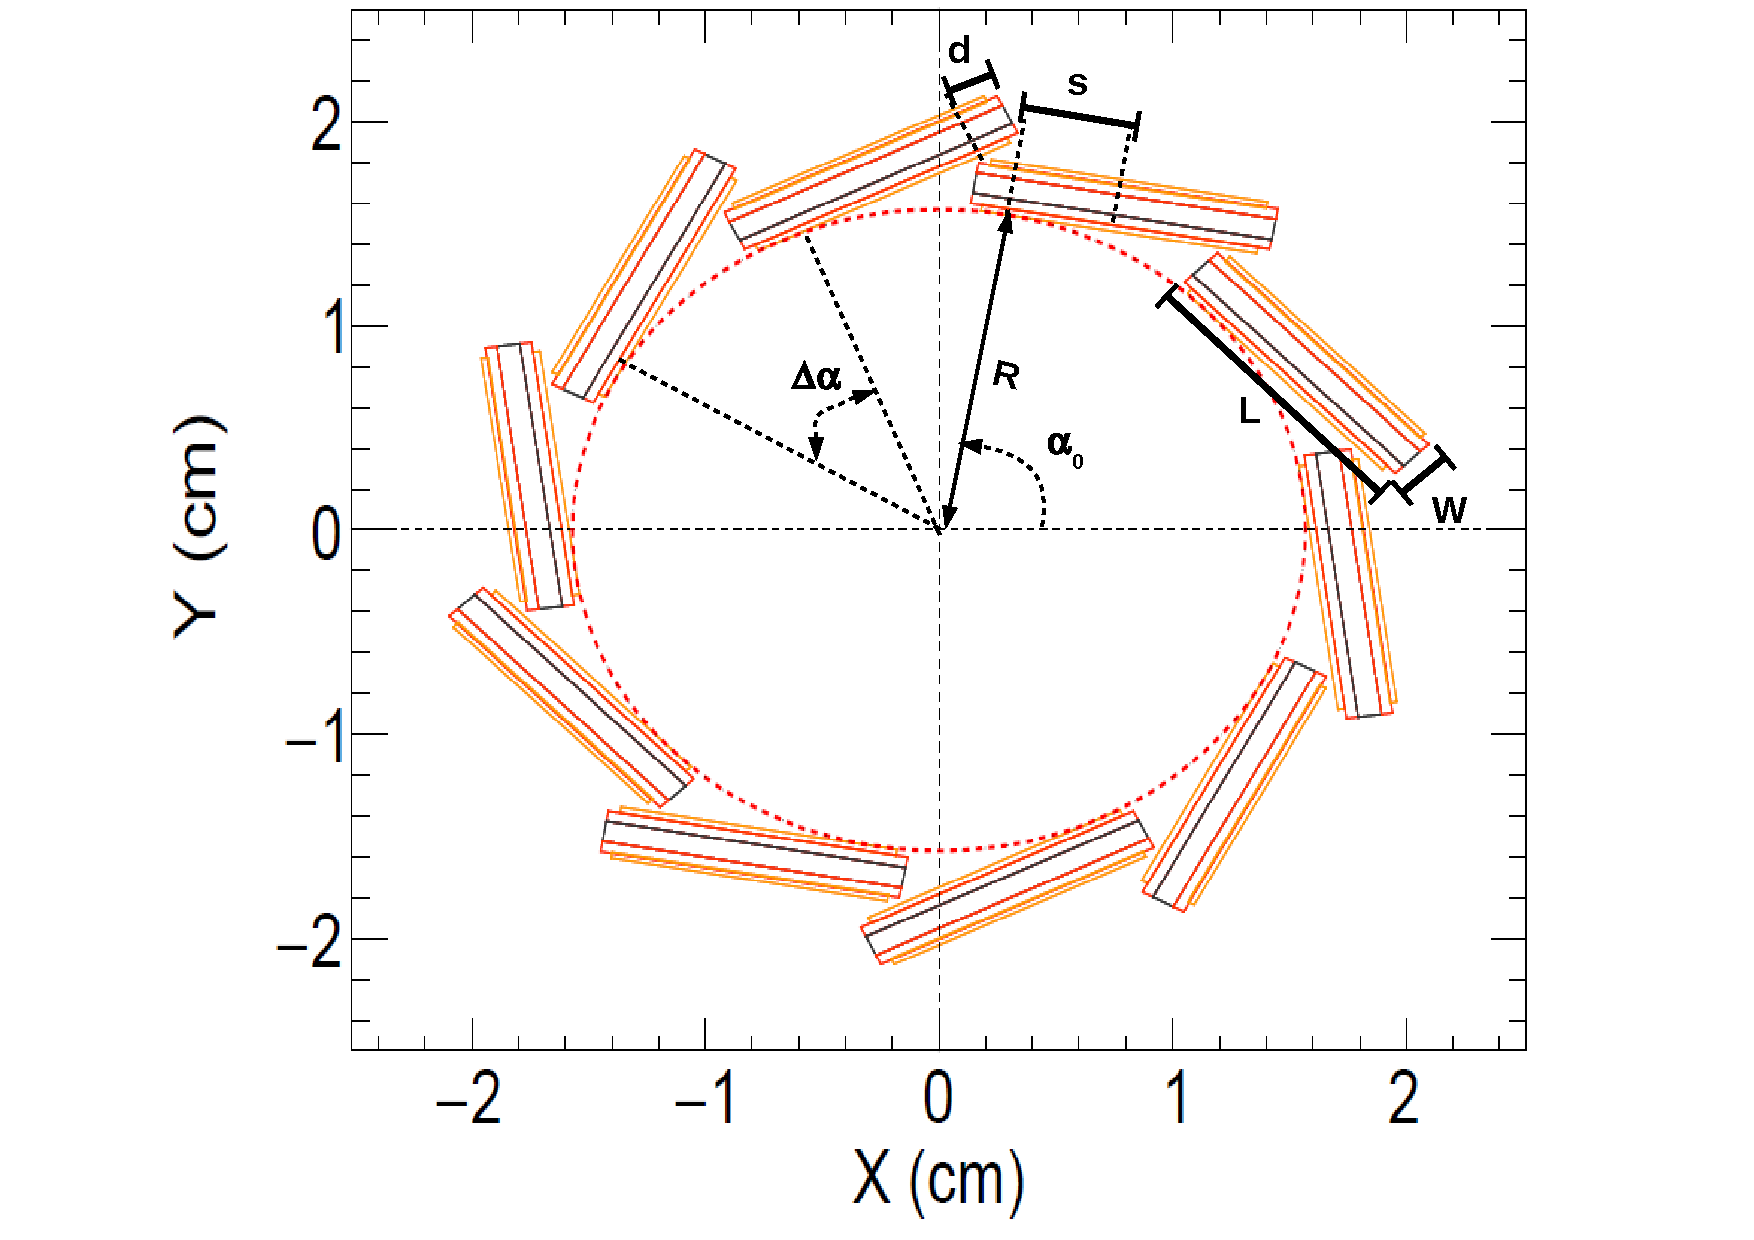
\includegraphics[width=0.9\textwidth]{figures/Spiral_Mosaic.pdf}
  \caption{Spiral plane ladder mosaic configuration.}
  \label{fig:Spiral_Plane_ladder_mosaic}
\end{figure}

\begin{itemize}
 \item  {\bf Spiral configuration}: 
   \begin{eqnarray}
     \label{eq:spiral_overlap}
     \frac{d}{L}   &=& 1 - \left(\frac{1 - \cos(\Delta\alpha)}{\sin(\Delta\alpha)}\right) \left(\frac{w + 2R}{L}\right) \\
     \label{eq:spiral_shift}
     \frac{s}{L}   &=& \left(1 - \frac{d}{L}\right) \left( \frac{R - (R + w)\cos(\Delta\alpha)}{ (1 - \cos(\Delta\alpha))(w + 2R)} \right) \\
     \Delta\alpha  &=& \frac{2\pi}{N_{\rm ladders}}
   \end{eqnarray}
   
   \item  {\bf Alternating configuration}: 
   \begin{eqnarray}
   \label{eq:alternating_overlap}
     \frac{d}{L}   &=& \frac{L(1 + \cos(\Delta\alpha)) - 2(w + R)\sin(\Delta\alpha)}{2L} \\
     \label{eq:alternating_shift}
     \frac{s}{L}   &=& \frac{(1 + w/R) [1 + (1 - 2\frac{d}{L})\cos(\Delta\alpha)]}{1 - 2\frac{d}{L} + \cos(\Delta\alpha)} \\
     \Delta\alpha  &=& \frac{2\pi}{N_{\rm ladders}/2}
   \end{eqnarray}
\end{itemize}
\noindent
Where $N_{\rm ladders}$ is the number of ladders.

\begin{figure}
  \centering
  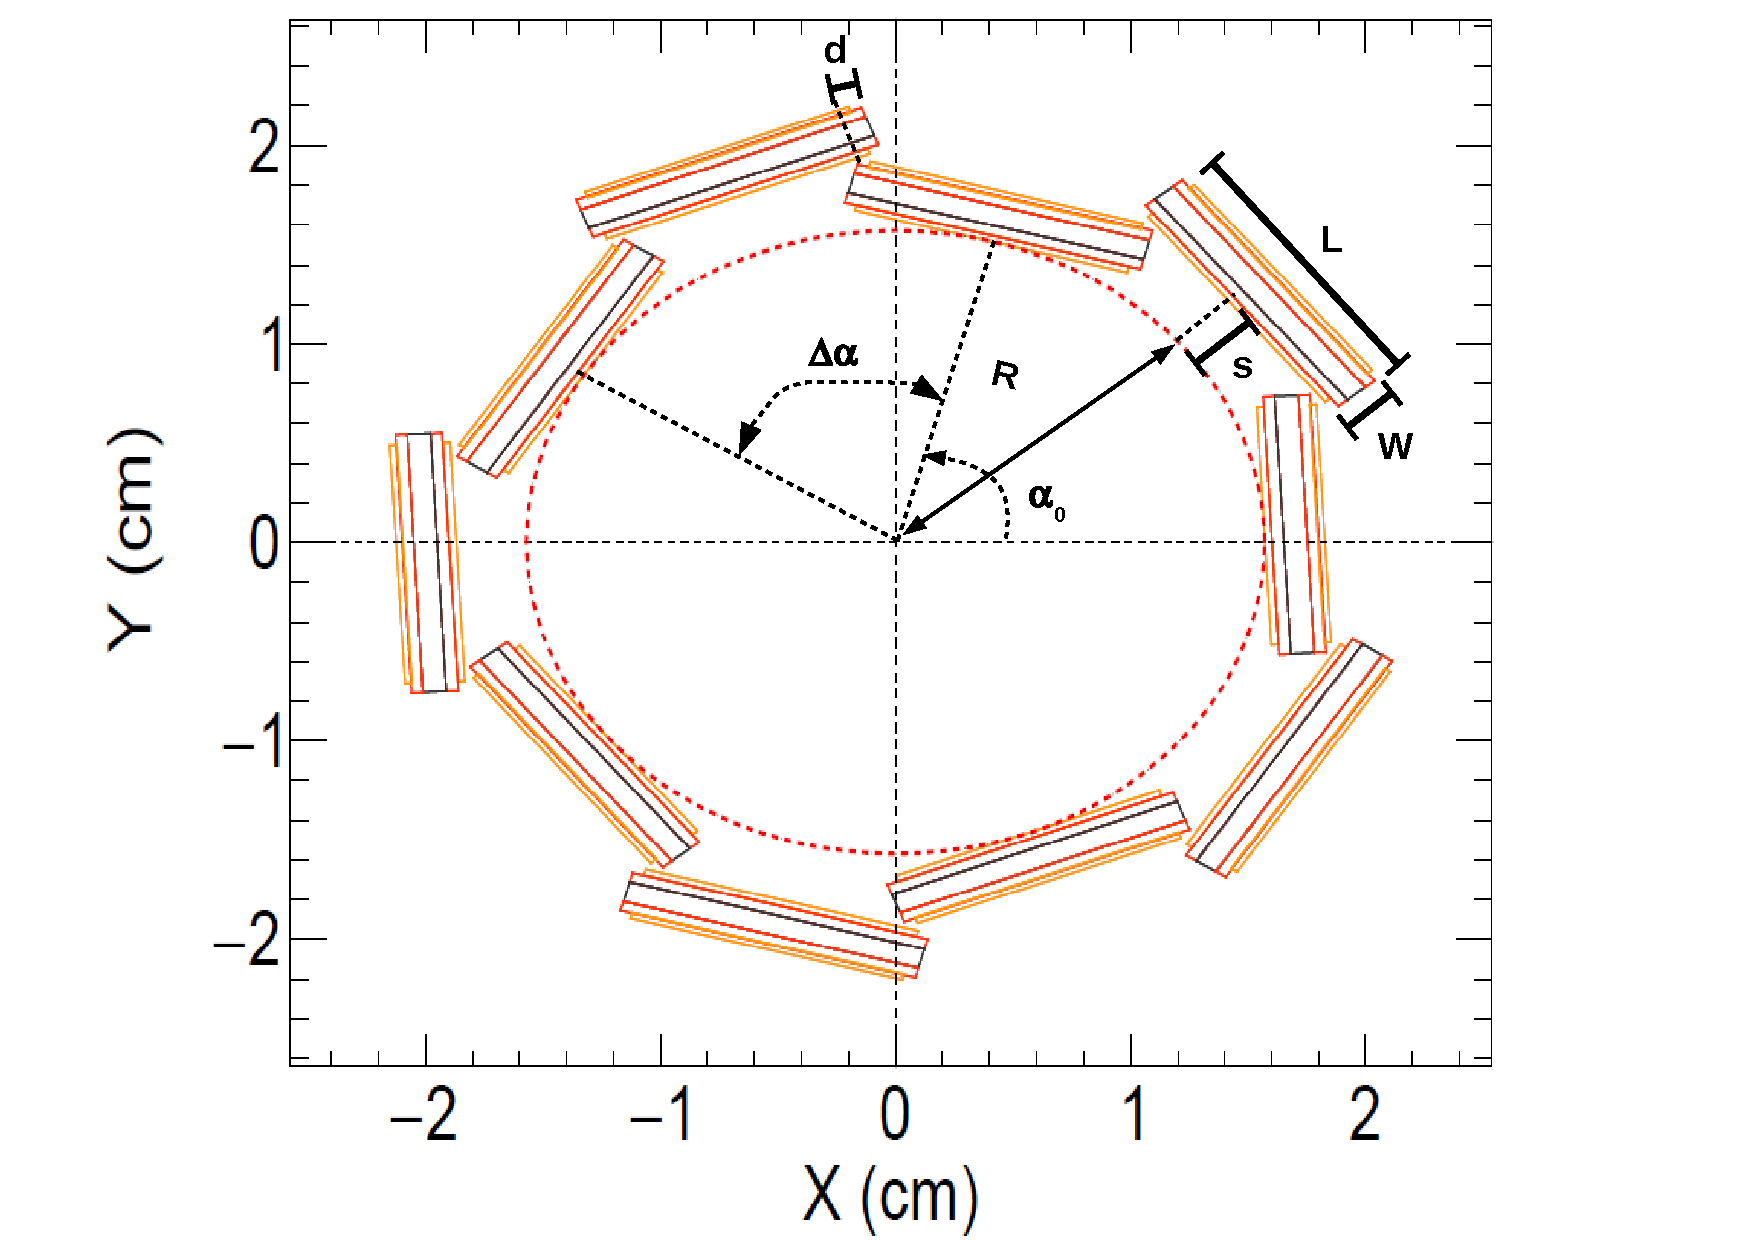
\includegraphics[width=0.9\textwidth]{figures/Alternating_Mosaic.pdf}
  \caption{Alternating plane ladder mosaic configuration.}
  \label{fig:Alternating_Plane_ladder_mosaic}
\end{figure}

~\\
The syntax to specify such structures is as follows.

~\\
\noindent
{\tt BeginMosaicLadderPlane} \\
$~~~~~${\tt LadderName        string                   $~~~~~~~~~~~~$   // (Mandatory)} \\
$~~~~~${\tt LadderMosaic      string                     $~~~~~~~~~~$   // (Mandatory)} \\
$~~~~~${\tt LadderPosition    x  y  z units                     $~~~$   // (Mandatory)} \\
$~~~~~${\tt LadderRotAngles   $\alpha_x$  $\alpha_y$  $\alpha_z$ units  // (Optional)}  \\
$~~~~~${\tt LadderVarPar      string                     $~~~~~~~~~~$   // (Mandatory)} \\
$~~~~~${\tt LadderRadius      value units                    $~~~~~$    // (Mandatory)} \\
$~~~~~${\tt LadderOverlap     value units                    $~~~~~$    // (Mandatory)} \\
$~~~~~${\tt LadderClearanceH  value units                       $~~$    // (Optional)} \\
$~~~~~${\tt LadderClearanceV  value units                       $~~$    // (Optional)} \\
$~~~~~${\tt LadderAlpha0      value units                   $~~~~~~$    // (Optional)} \\
$~~~~~${\tt LadderN           value              $~~~~~~~~~~~~~~~~~$    // (Mandatory)} \\
$~~~~~${\tt LadderShift       value                  $~~~~~~~~~~~~~$    // (Optional)} \\
$~~~~~${\tt LadderShiftFix    bool                      $~~~~~~~~~~~$    // (Optional)} \\
$~~~~~${\tt BeginPlane} \\
$~~~~~~~${\tt Name             string                   $~~~~~~~~~~~~$   // (Mandatory)} \\
$~~~~~~~${\tt Position         x  y  z units                     $~~~$   // (Mandatory)} \\
$~~~~~~~${\tt Thickness        value  units                       $~~$   // (Mandatory, value > 0)} \\
$~~~~~~~${\tt Material         string                       $~~~~~~~~$   // (Mandatory)} \\
$~~~~~~~${\tt XOX0             value                   $~~~~~~~~~~~~~$   // (Optional)}  \\
$~~~~~~~${\tt widthU           value units                     $~~~~~$   // (Mandatory, value > 0)} \\
$~~~~~~~${\tt widthV           value units                     $~~~~~$   // (Mandatory, value > 0)} \\
$~~~~~~~${\tt IsSensitive      bool                          $~~~~~~~$   // (Mandatory)} \\
$~~~~~~~${\tt ResolutionU      value units                               // (Optional, value > 0)} \\
$~~~~~~~${\tt ResolutionV      value units                               // (Optional, value > 0)} \\
$~~~~~~~${\tt Resolution       value units                               // (Optional, value > 0)} \\
$~~~~~~~${\tt ROtime           value units                      $~~~~$   // (Optional, value > 0)} \\
$~~~~~~~${\tt Efficiency       value                          $~~~~~~$   // (Optional, 0 <= value <= 1)} \\
$~~~~~~~${\tt InsensFracVneg   value                              $~~$   // (Optional, default is zero)} \\
$~~~~~~~${\tt InsensFracVpos   value                              $~~$   // (Optional, default is zero)} \\
$~~~~~~~${\tt BkgRate          value units                       $~~~$   // (Optional, default is zero)} \\
$~~~~~~~${\tt SystemName       string                          $~~~~~$   // (Optional)} \\
$~~~~~~~${\tt LayerName        string                         $~~~~~~$   // (Optional)} \\
$~~~~~~~${\tt ResolutionModel  string                                    // (Optional)} \\
$~~~~~~~${\tt EfficiencyModel  string                                    // (Optional)} \\
$~~~~~${\tt EndPlane} \\
$~~~~~$ ... \\
{\tt EndMosaicLadderPlane}

~\\
As in the case of the plane ladder, an indefinite number of planes can be specified. Out of this list the system
will calculate $L$ and $w$ (see figures~\ref{fig:Spiral_Plane_ladder_mosaic} and~\ref{fig:Alternating_Plane_ladder_mosaic}) 
as the maximum width and total thickness of the ladder adding a clearance of {\tt LadderClearanceH} and {\tt LadderClearanceV}, 
respectively. The {\tt LadderMosaic} parameter defines the type of structure to build, it can only have the values "Spiral" or 
"Alternating". Another important parameter is {\tt LadderVarPar}, which is the parameter to be calculated out of the others using 
Eq.~\ref{eq:spiral_overlap} or~\ref{eq:alternating_overlap}. This parameter can have either the value "Overlap" or "Radius". 
In the first (second) case the overlap $d/L$ (radius $R$) is calculated fixing all the other parameters. The shift $s/L$ is 
then calculated from Eq~\ref{eq:spiral_shift} or~\ref{eq:alternating_shift}. If the boolean parameter {\tt LadderShiftFix} is set 
to {\tt true}, the shift will be fixed to the specified value {\tt LadderShift}.

\subsubsection{Petal ladder mosaic}

A petal ladder mosaic is complex structure made from petal ladders to resemble a disk as shown in figure~\ref{fig:Petal_ladder_mosaic}.
The syntax to specify such structure is as follows.

~\\
\noindent
{\tt BeginMosaicLadderPetal} \\
$~~~~~${\tt LadderName        string                   $~~~~~~~~~~~~$   // (Mandatory)} \\
$~~~~~${\tt LadderPosition    x  y  z units                     $~~~$   // (Mandatory)} \\
$~~~~~${\tt LadderRotAngles   $\alpha_x$  $\alpha_y$  $\alpha_z$ units  // (Optional)}  \\
$~~~~~${\tt LadderRadius      value units                    $~~~~~$    // (Mandatory)} \\
$~~~~~${\tt LadderAlpha0      value units                   $~~~~~~$    // (Optional)} \\
$~~~~~${\tt LadderN           value              $~~~~~~~~~~~~~~~~~$    // (Mandatory)} \\
$~~~~~${\tt LadderShift       value units                  $~~~~~~~$    // (Optional)} \\
$~~~~~${\tt BeginPetal} \\
$~~~~~~~${\tt Name             string                   $~~~~~~~~~~~~$   // (Mandatory)} \\
$~~~~~~~${\tt Position         x  y  z units                     $~~~$   // (Mandatory)} \\
$~~~~~~~${\tt Thickness        value  units                       $~~$   // (Mandatory, value > 0)} \\
$~~~~~~~${\tt Material         string                       $~~~~~~~~$   // (Mandatory)} \\
$~~~~~~~${\tt XOX0             value                   $~~~~~~~~~~~~~$   // (Optional)}  \\
$~~~~~~~${\tt bottomWidth      value units                               // (Mandatory, value > 0)} \\
$~~~~~~~${\tt topWidth         value units                       $~~~$   // (Mandatory, value > 0)} \\
$~~~~~~~${\tt Height           value units                     $~~~~~$   // (Mandatory, value > 0)} \\
$~~~~~~~${\tt IsSensitive      bool                          $~~~~~~~$   // (Mandatory)} \\
$~~~~~~~${\tt ResolutionU      value units                               // (Optional, value > 0)} \\
$~~~~~~~${\tt ResolutionV      value units                               // (Optional, value > 0)} \\
$~~~~~~~${\tt Resolution       value units                               // (Optional, value > 0)} \\
$~~~~~~~${\tt ROtime           value units                      $~~~~$   // (Optional, value > 0)} \\
$~~~~~~~${\tt Efficiency       value                          $~~~~~~$   // (Optional, 0 <= value <= 1)} \\
$~~~~~~~${\tt InsensFracVneg   value                              $~~$   // (Optional, default is zero)} \\
$~~~~~~~${\tt InsensFracVpos   value                              $~~$   // (Optional, default is zero)} \\
$~~~~~~~${\tt BkgRate          value units                       $~~~$   // (Optional, default is zero)} \\
$~~~~~~~${\tt SystemName       string                          $~~~~~$   // (Optional)} \\
$~~~~~~~${\tt LayerName        string                         $~~~~~~$   // (Optional)} \\
$~~~~~~~${\tt ResolutionModel  string                                    // (Optional)} \\
$~~~~~~~${\tt EfficiencyModel  string                                    // (Optional)} \\
$~~~~~${\tt EndPetal} \\
$~~~~~$ ... \\
{\tt EndMosaicLadderPetal}

~\\
As in the case of the plane ladder, an indefinite number of petals can be specified taking care that they not overlap. 
In figure~\ref{fig:Petal_ladder_mosaic} can be appreciated the parameters needed to build this structure. {\tt LadderRadius} 
is $R$, {\tt LadderAlpha0} is $\alpha_0$, and {\tt LadderN} is half the number of petals. The {\tt LadderShift} parameter in 
this case is a shift along the disk normal vector. The petals marked by "$+$" ("$-$") in figure~\ref{fig:Petal_ladder_mosaic}
are shifted by $+${\tt LadderShift} ($-${\tt LadderShift}) along this direction.

\begin{figure}
  \centering
  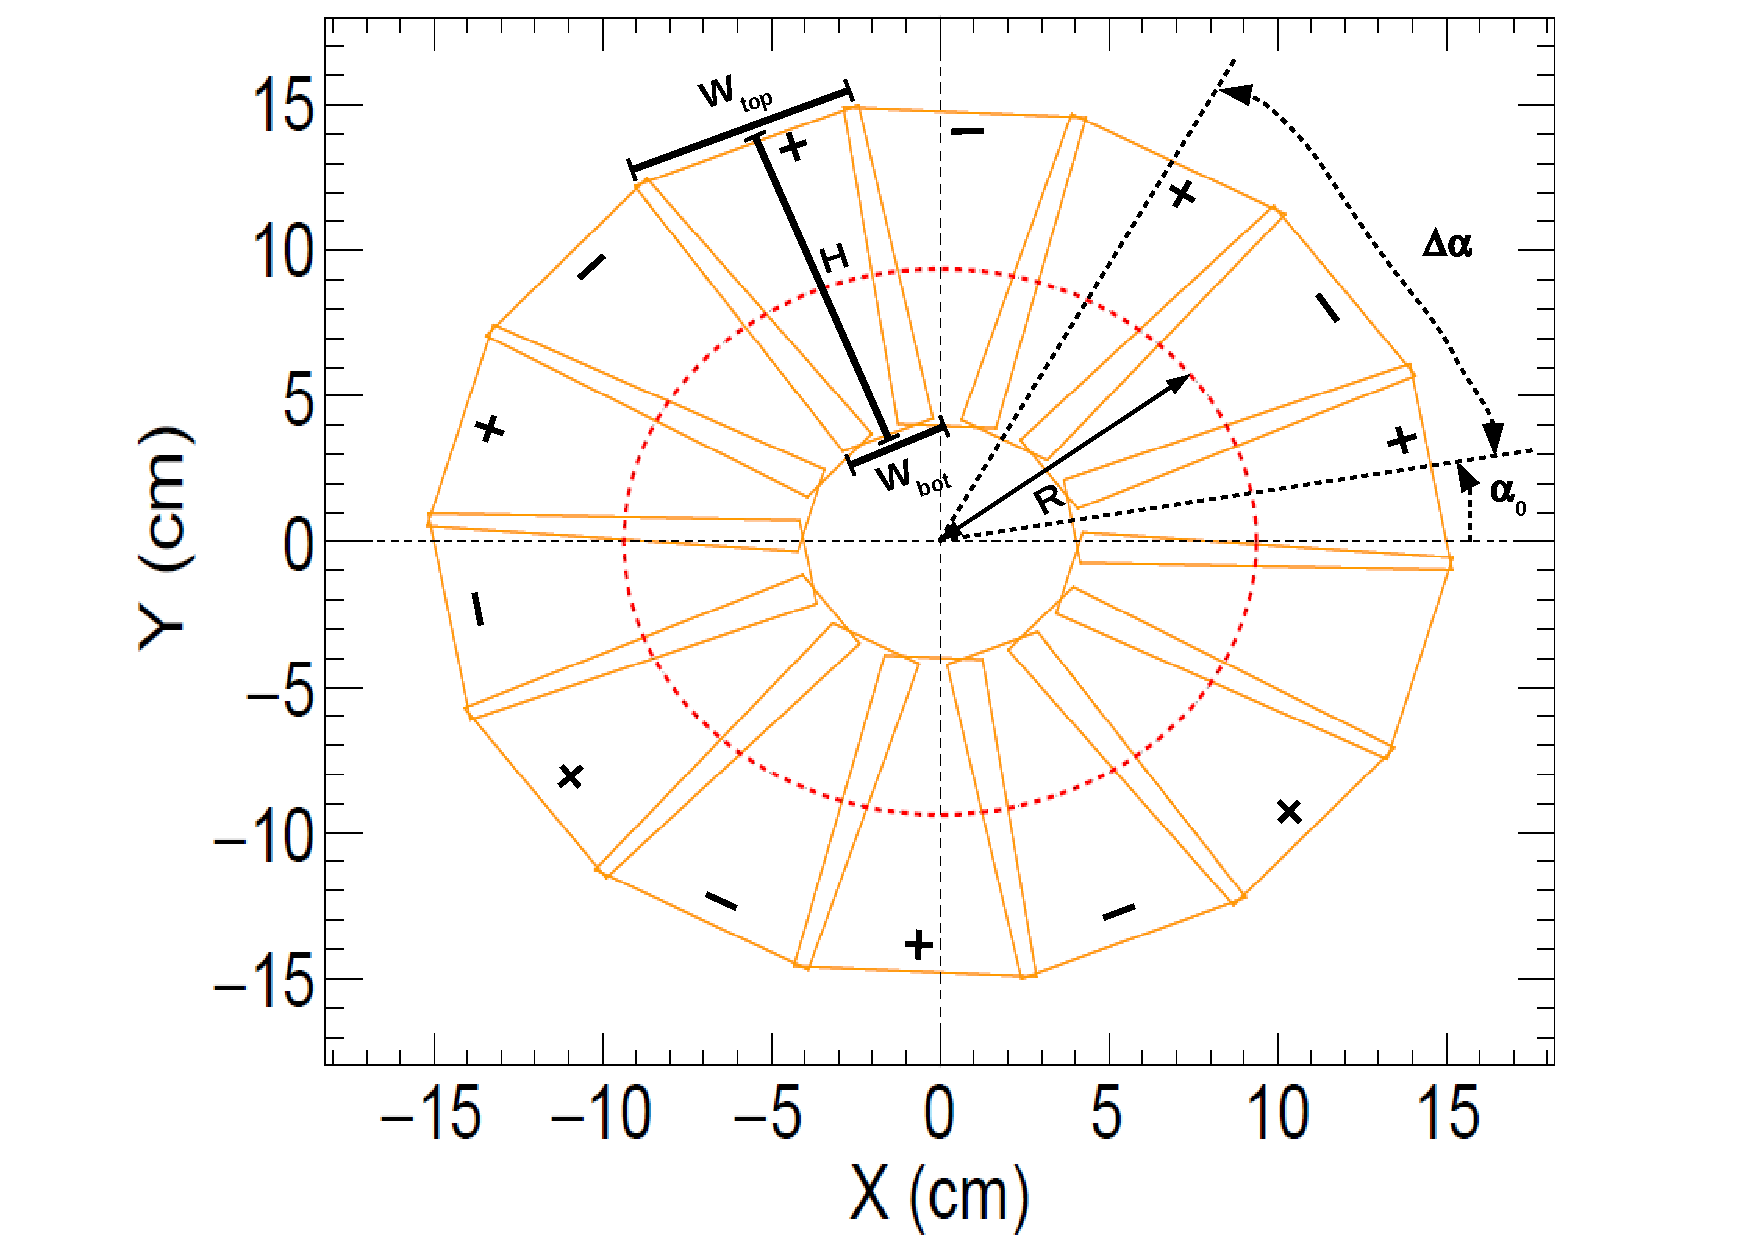
\includegraphics[width=0.9\textwidth]{figures/Petal_Mosaic.pdf}
  \caption{Petal ladder mosaic configuration.}
  \label{fig:Petal_ladder_mosaic}
\end{figure}

~\\
~\\
\noindent
This completes the kind of geometrical structures that can be build in {\guari}. 

\subsection{Intrinsic resolution model}

By default in {\guari} the spatial resolution of any measurement is equal to the intrinsic resolution ({\tt ResolutionU/V}) of the sensitive element. 
Moreover, the spatial resolution of a sensor could depend as well on the intersection coordinates and momentum with the sensor's main surface, and on 
some other parameters. This is a reason behind of the resolution model.

\subsubsection{Gas detector resolution model}
\label{subsubsec:GasDet_resolModel}

For the moment there is only one resolution model implemented, mainly to model the spatial resolution of gas detectors as a TPC or a drift-chamber. 
The syntax is as follows.

~\\
\noindent
{\tt BeginTPCResolutionModel} \\
$~~~~~${\tt Name        string                    $~~~~~~~~~~~$    // (Mandatory)} \\
$~~~~~${\tt A\_U         value units                  $~~~~~~~$    // (Mandatory, value > 0)} \\
$~~~~~${\tt B\_U         value units                  $~~~~~~~$    // (Mandatory, value > 0)} \\
$~~~~~${\tt C\_U         value units                  $~~~~~~~$    // (Mandatory, value > 0)} \\
$~~~~~${\tt A\_V         value units                  $~~~~~~~$    // (Mandatory, value > 0)} \\
$~~~~~${\tt B\_V         value units                  $~~~~~~~$    // (Mandatory, value > 0)} \\
{\tt EndTPCResolutionModel}

~\\
The {\tt Name} parameter defines the resolution model. Any sensor with its parameter {\tt ResolutionModel} set 
to this name will use this resolution model. The resolution is calculated as follows,

\begin{eqnarray}
  {\rm ResolutionU}^2 &=& {\rm A_U}^2 + {\rm B_U}^2\sin\phi + {\rm C_U}\sin\theta\times z, \\
  {\rm ResolutionV}^2 &=& {\rm A_V}^2 + {\rm B_V}\times z;
\end{eqnarray}
\noindent
where $\theta$, $\phi$ and $z$ are the polar and azimuthal angles of the momentum and the z-coordinate at the intersection of the track with 
the volume main surface.

~\\
\noindent
See section~\ref{subsubsec:Example3} for an example illustrating of this resolution model.

\subsection{Detection efficiency model}

As in the case of the spatial resolution, by default in {\guari} the detection efficiency of any measurement is equal to the intrinsic detection efficiency ({\tt Efficiency}) 
of the sensitive element. Moreover, the detection efficiency of a sensor could depend as well on the intersection coordinates and momentum with the sensor's main surface, and 
on some other parameters. This is a reason behind of the efficiency model.

~\\
~\\
\noindent
For the time being there is no Efficiency model implemented in {\guari}, only a base class.

\subsection{Systems configuration}

It is useful to label a set of geometry elements as a system. The usefulness has already being shown the examples of 
sections~\ref{subsubsec:Example2} and ~\ref{subsubsec:Example4}, for the material budget studies. The syntax to define the 
systems configurations is as follows.

~\\
\noindent
{\tt BeginSystemsConfiguration} \\
$~~~~~${\tt BeginSystem} \\
$~~~~~~~${\tt Name             string       $~~~~~~~~~~~~~~~~~~~~$   // (Mandatory)} \\
$~~~~~~~${\tt LayersList       string1  string2  ....                // (Mandatory)} \\
$~~~~~${\tt EndSystem} \\
$~~~~~$ ... \\
{\tt EndSystemsConfiguration}

~\\
\noindent
where {\tt LayerList} is a list of geometry element {\tt LayerName}. The user can define as many systems as needed, but 
no two systems can share the same {\tt LayerName}.

\subsection{Telescope-DUT configuration}
\label{subsec::TelDUT_config}

In some cases it is interesting to understand the pointing precision of tracks reconstructed with a set of sensitive elements (Telescope) 
toward some other elements (DUTs). The use of this feature has been illustrated in examples of sections~\ref{subsubsec:Example1} and ~\ref{subsubsec:Example2}.
The syntax for configuring a Telescope-DUT setup is as follows.

~\\
\noindent
{\tt BeginBeamTestConfiguration} \\
$~~~~~${\tt TelescopeLayersList  string1   string2  string3  ... // (Mandatory)} \\
$~~~~~${\tt DUTLayersList        string1   string2  string3  ... $~~~~~$ // (Mandatory)} \\
{\tt EndBeamTestConfiguration}

~\\
\noindent
where {\tt TelescopeLayersList} and {\tt DUTLayersList} are lists with the {\tt LayerName}s which define the Telescope and DUTs, respectively.

\subsection{Track-Finder algorithms}
\label{subsec::TrkFinder_config}

When calculating the tracking efficiency a co-called {\tt TrackFinderAlgo} object has to be specified. Each such object will be used 
for a certain regions of the tracker. No two {\tt TrackFinderAlgo} can have overlapping regions, in such a case the program will crash with 
an error message.

For the time being only one track-finder object has been implemented, the so-called FPCCDTrackFinderAlgo. Its syntax is described in the section 
below.

\subsubsection{FPCCD Track-Finder algorithm}

The syntax for this track finder is as follows,

~\\
\noindent
{\tt BeginFPCCDTrackFinderAlgo}
$~~~~~${\tt Name              string                (Mandatory)} \\
$~~~~~${\tt PtMin             val units // val > 0  (Mandatory)} \\
$~~~~~${\tt NhitsMin          val       // val > 0  (Mandatory)} \\
$~~~~~${\tt PurityMin         val       // val > 0  (Optional, default value is 1)} \\
$~~~~~${\tt Chi2OndfSeed      val       // val > 0  (Optional, default value is 3)} \\
$~~~~~${\tt Chi2OndfAdd       val       // val > 0  (Optional, default value is 3)} \\
$~~~~~${\tt NfakesMaxSeeding  val       // val >= 0 (Optional, default value is 0)} \\
$~~~~~${\tt NmcSeedEffic      val       // val >= 0 (Optional, default value is 1000)} \\
$~~~~~${\tt BeginTrackFinderRegion} \\
$~~~~~~~${\tt positionRangeX      min  max  units // max > min (Optional)} \\
$~~~~~~~${\tt positionRangeY      min  max  units // max > min (Optional)} \\
$~~~~~~~${\tt positionRangeZ      min  max  units // max > min (Optional)} \\
$~~~~~~~${\tt positionRangeR      min  max  units // max > min (Optional)} \\
$~~~~~~~${\tt positionRangeTheta  min  max  units // max > min (Optional)} \\
$~~~~~~~${\tt positionRangePhi    min  max  units // max > min (Optional)} \\
$~~~~~~~${\tt momentumRangeP      min  max  units // max > min and both >= 0 (Optional)} \\
$~~~~~~~${\tt momentumRangeTheta  min  max  units // max > min (Optional)} \\
$~~~~~~~${\tt momentumRangePhi    min  max  units // max > min (Optional)} \\
$~~~~~${\tt EndTrackFinderRegion} \\
$~~~~~${\tt BeginSystems} \\
$~~~~~~~${\tt System   string} \\
$~~~~~~~${\tt ...} \\
$~~~~~${\tt EndSystems} \\
$~~~~~${\tt BeginSeedConfigs} \\
$~~~~~~~${\tt SeedConfig   string1  string2  string3 ...} \\
$~~~~~~~${\tt ...} \\
$~~~~~${\tt EndSeedConfigs} \\
{\tt EndFPCCDTrackFinderAlgo}

~\\
\noindent
where 

\begin{itemize}
  \item  {\tt PtMin} is the $p^{\rm min}_t$ cut for seeding.
  
  \item  {\tt NhitsMin} is the minimum number of hits allowed to reconstruct the track.
  
  \item  {\tt PurityMin} is the minimum allowed value of the track purity, defined as (\# good hits)/(\# hits). It defined the maximum number of 
  fake hits in the track as follows, $N^{\rm max}_{\rm fake} = N_{hit}(1 - {\rm PurityMin})$.

  \item  {\tt Chi2OndfSeed} is the $(\chi^2/ndf)_{\rm max}$ for seed tracks.
  
  \item  {\tt Chi2OndfAdd} is the $\chi^2/ndf$ maximum cut for track-hit association.
  
  \item  {\tt NfakesMaxSeeding} is the maximum allowed number of fake hits for seeding.
  
  \item  {\tt NmcSeedEffic} is the number of samplings for the seeding efficiency MC calculation.
\end{itemize}

The region where this {\tt TrackFinderAlgo} object will be used is specified in the block between {\tt BeginTrackFinderRegion} and 
{\tt EndTrackFinderRegion}. The region is specified in terms of the track origin and momentum. At least of the possible ranges has to be specified.

The systems considered for the tracking is specified in the block between {\tt BeginSystems} and {\tt EndSystems}. Each entry in this block 
should be the full system name ({\tt SystemName}).

Finally, the seeding configurations are specified in the block between {\tt BeginSeedConfigs} and {\tt EndSeedConfigs}. Every seed 
configuration is specified by listing sets of three layer-names ({\tt LayerName}).

~\\
\noindent
See section~\ref{subsubsec:FPCCDTrkEffic_calculation} for a detailed explanation of the parameters above as well as the process for the tracking efficiency calculation.

\subsection{Track cuts}

In some cases it is needed to perform cuts on the number of hits within a system for tracks in some ranges of its momentum components $(p,\theta,\phi)$. 
The syntax is as follows.

~\\
\noindent
{\tt BeginTrackCuts} \\
$~~~~~${\tt SystemName        string        $~~~~~~~$   // (Mandatory)} \\
$~~~~~${\tt BeginCut} \\
$~~~~~~~${\tt pRange           min  max  units  $~~~$   // (Optional)} \\
$~~~~~~~${\tt phiRange         min  max  units    $~$   // (Optional)} \\
$~~~~~~~${\tt thetaRange       min  max  units          // (Optional)} \\
$~~~~~~~${\tt NhitsRange       min  max  units          // (Mandatory)} \\
$~~~~~${\tt EndCut} \\
$~~~~~$ ... \\
{\tt EndTrackCuts}

~\\
\noindent
Where SystemName is the name of the system in which the cut on the number of hits will be applied. The data structure between {\tt BeginCut} and {\tt EndCut} 
implement the cut. The $p$, $\theta$ and $\phi$ ranges ({\tt pRange}, {\tt phiRange} and {\tt thetaRange}, respectively) identify the range of momentum where the 
cut {\tt NhitsRange} will be applied. While implementing a cut, at least one range, either $p$, $\theta$ or $\phi$ range has to be specified.

\subsection{Global hit rate scaling}
\label{subsec:global_bkgrate_scaling}

This is a feature is for globally scaling the hit rates on all the sensitive elements of the geometry. This could be useful to study tracking performances 
in terms of the hit rate labels. The syntax for this feature is very simple.

~\\
\noindent
{\tt GlobalBkgRateScaling:  scaling} \\

~\\
\noindent
where the {\tt scaling} has to be $\geq 0$. If not the program will crash with an error message.

~\\
~\\
\noindent
This concludes all what is needed to build a geometry. Lets now continue to the next section where the analysis configurations will be described.


\section{Analysis configuration}
\label{sec:analysis_config}

In this section is described the syntax for the main data-card file. The items below describe general parameters for all the analysis which are either mandatory or optional. 
Later sections will describe the syntax to setup the different analysis. See section~\ref{subsec:Some_examples} for some examples illustrating this features.

\begin{itemize}
 \item  {\bf Verbosity}: the {\tt Verbose:} parameter is a boolean optional parameter (default value is false). It is a flag used for debugging. 
 If true is several print-outs will be displayed.

 \item  {\bf Particle parameters}:
 \begin{itemize}
   \item {\tt ParticleType:} a mandatory parameter. Possible values is the list of stable particles: {\tt e-} or {\tt e+} (electron/positron), 
   {\tt mu+} or {\tt mu-} (muon), {\tt pi+} or {\tt pi-} (pion), {\tt K+} or {\tt K-} (Kaon), {\tt p+} or {\tt p-} (proton), {\tt 4He++} (double-ionized Helium-4).
   
   \item  {\tt ParticleOrigin:} a mandatory parameter. It is the point $(x,y,z)$ from which the particle is going to be tracker in the process of
   geometry navigation.
 \end{itemize}
   
 \item  {\bf Pivot point}: {\tt ReferencePoint} is a mandatory parameter. Trajectories are always parameterized in terms of some quantities defined with respect to
 a pivot-point.
 
 \item  {\bf MC seed}: {\tt MCSeed:} is an optional parameter. This seed is used to initialize the random-generator used for the MC calculation of the seeding 
 efficiency (c.f. sec.~\ref{subsubsec:FPCCDTrkEffic_calculation}).
 
 \item  {\bf Include $E_{\rm loss}$ calculation}: the {\tt IncludeEloss:} parameter is a boolean optional parameter (default value is true). It is a flag used for including 
 the $E_{\rm loss}$ fluctuations in the measurements covariance matrix (c.f. sec.~\ref{subsec:TrkParm_CovMatrix_calculation}).
 
 \item  {\bf Tunning the $E_{\rm loss}$ fluctuations model}: the $\kappa$ parameter in the $E_{\rm loss}$ fluctuations model (c.f. eq.~\ref{eq:sigmaEloss}) can be modified if needed 
 with the following syntax,
 
 ~\\
 \noindent     
 {\tt KappaElossFluctuation:  value units} \\
 ~\\
 \noindent
 where the units should be those of energy.
 
 
 \item {\bf The momentum scan parameters}: a set of values for the momentum or energy variable (see below), polar variable ($\theta$, $\cos\theta$ or $\eta$) and azimuthal angle ($\phi$). 
 All of them can be specified as a range or as a set of discrete values. Here below are the possibilities
 \begin{itemize}
   \item {\bf Momentum or energy variable}: the momentum or energy variable can be specified in four ways, either $p$ (momentum), $E$ (energy), $E_{kin}$ (kinetic energy) or $E_{kin}/u$ 
   (kinetic energy per nucleon); where the last one is only useful when studying ionized heavy nuclei. For each of them the either a list of discrete values or 
   a range can be specified. The syntax for all these possibilities is as follows,
   
   \begin{itemize}
     \item {\bf List of discrete momentum values}:
     
     \noindent
     {\tt MomentumValues: value1  value2  value3 ... units } \\
     \noindent
     where as many values as needed can be specified. At least one value needs to be specified.
     ~\\
     
     \item {\bf Momentum range}: syntax is as follows,
     ~\\
     \noindent     
     {\tt BeginMomentumScan} \\
     $~~~~${\tt Nbins   integer $~~$ // (Mandatory)} \\
     $~~~~${\tt pMin    value units  // (Mandatory)} \\
     $~~~~${\tt pMax    value units  // (Mandatory)} \\
     {\tt EndMomentumScan}
     ~\\
     
     \item {\bf List of discrete energy values}:
     
     \noindent
     {\tt EnergyValues: value1  value2  value3 ... units } \\
     \noindent
     where as many values as needed can be specified. At least one value needs to be specified.
     ~\\
     
     \item {\bf Energy range}: syntax is as follows,
     ~\\
     \noindent     
     {\tt BeginEnergyScan} \\
     $~~~~${\tt Nbins   integer $~~$ // (Mandatory)} \\
     $~~~~${\tt EMin    value units  // (Mandatory)} \\
     $~~~~${\tt EMax    value units  // (Mandatory)} \\
     {\tt EndEnergyScan}
     ~\\
     
     \item {\bf List of discrete kinetic energy values}:
     
     \noindent
     {\tt EkinValues: value1  value2  value3 ... units } \\
     \noindent
     where as many values as needed can be specified. At least one value needs to be specified.
     ~\\
     
     \item {\bf Kinetic energy range}: syntax is as follows,
     ~\\
     \noindent     
     {\tt BeginEkinScan} \\
     $~~~~${\tt Nbins   integer $~~$ // (Mandatory)} \\
     $~~~~${\tt EkinMin    value units  // (Mandatory)} \\
     $~~~~${\tt EkinMax    value units  // (Mandatory)} \\
     {\tt EndEkinScan}
     ~\\
     
     \item {\bf List of discrete kinetic energy per nucleon values}:
     
     \noindent
     {\tt EkinPerUValues: value1  value2  value3 ... units } \\
     \noindent
     where as many values as needed can be specified. At least one value needs to be specified.
     ~\\
     
     \item {\bf Kinetic energy per nucleon range}: syntax is as follows,
     ~\\
     \noindent     
     {\tt BeginEkinPerUScan} \\
     $~~~~${\tt Nbins   integer $~~$ // (Mandatory)} \\
     $~~~~${\tt EkinPerUMin    value units  // (Mandatory)} \\
     $~~~~${\tt EkinPerUMax    value units  // (Mandatory)} \\
     {\tt EndEkinPerUScan}
     ~\\
     
   \end{itemize}
   If no $p$, $E$, $E_{kin}$ or $E_{kin}/u$ values are specified, then a single $p = 2~{\rm GeV/c}$ value will be will be used. Non of the momentum or energy values can be negative, if so the program will 
   crash with an error message. Furthermore, in the case of specifying energy values, $E$, all the specified values have to be larger than the particle mass, otherwise the program will crass with an error 
   message.
   ~\\
 
   \item {\bf Polar variable}: the polar variable can be specified in three ways, either $\theta$, $\cos\theta$ or $\eta$. For each of them the either a list of discrete values or 
   a range can be specified. The syntax for all these possibilities is as follows,
   
   \begin{itemize}
     \item {\bf List of discrete $\theta$ values}:
     
     \noindent
     {\tt PolarAngleValues: value1  value2  value3 ... units } \\
     \noindent
     where as many values as needed can be specified. At least one value needs to be specified.
     ~\\
     
     \item {\bf $\theta$ Range}:
     ~\\
     \noindent     
     {\tt BeginPolarAngleScan} \\
     $~~~~${\tt Nbins       integer $~~~~~~$ // (Mandatory)} \\
     $~~~~${\tt thetaMin    value units      // (Mandatory)} \\
     $~~~~${\tt thetaMax    value units      // (Mandatory)} \\
     {\tt EndPolarAngleScan}
     ~\\
     
     \item {\bf List of discrete $\cos\theta$ values}:
     
     \noindent
     {\tt CosThetaValues: value1  value2  value3 ... units } \\
     \noindent
     where as many values as needed can be specified. At least one value needs to be specified.
     ~\\
     
     \item {\bf $\cos\theta$ Range}:
     ~\\
     \noindent     
     {\tt BeginCosThetaScan} \\
     $~~~~${\tt Nbins          integer $~~~~~~~~~$ // (Mandatory)} \\
     $~~~~${\tt costhetaMin    value units         // (Mandatory)} \\
     $~~~~${\tt costhetaMax    value units         // (Mandatory)} \\
     {\tt EndCosThetaScan}
     ~\\
     
     \item {\bf List of discrete $\eta$ values}:
     
     \noindent
     {\tt EtaValues: value1  value2  value3 ... units } \\
     \noindent
     where as many values as needed can be specified. At least one value needs to be specified.
     ~\\
     
     \item {\bf $\eta$ Range}:
     ~\\
     \noindent     
     {\tt BeginEtaScan} \\
     $~~~~${\tt Nbins     integer $~~~~$ // (Mandatory)} \\
     $~~~~${\tt etaMin    value units         // (Mandatory)} \\
     $~~~~${\tt etaMax    value units         // (Mandatory)} \\
     {\tt EndEtaScan}
     ~\\
     
   \end{itemize}
   
   \item {\bf Azimuthal angle}: 
   \begin{itemize}
     \item {\bf List of discrete values}: syntax is as follows,
     
     \noindent
     {\tt AzimuthalAngleValues: value1  value2  value3 ... units } \\
     \noindent
     where as many values as needed can be specified. At least one value needs to be specified.
     
     \item {\bf Range}: syntax is as follows,
     ~\\
     \noindent     
     {\tt BeginAzimuthalAngleScan} \\
     $~~~~${\tt Nbins     integer $~~~~$ // (Mandatory)} \\
     $~~~~${\tt phiMin    value units    // (Mandatory)} \\
     $~~~~${\tt phiMax    value units    // (Mandatory)} \\
     {\tt EndAzimuthalAngleScan}
   \end{itemize}
   
 \end{itemize}
 
 \item {\bf Momentum resolution representation}: In the case where $p$ or $p_{t}$ is part of the track parameters, its resolution can be 
 represented in different ways: $\sigma(p)/p$, $\sigma(p)$ or $\sigma(1/p)$. The default one is $\sigma(p)/p$. A parameter allows to select the 
 representation as {\tt MonResolRepresentation: string}, where {\tt string} can only have the values: {\tt sigma(Pt)/Pt}, {\tt sigma(Pt)} or 
 {\tt sigma(1/Pt)}, corresponding to the $\sigma(p)/p$, $\sigma(p)$ or $\sigma(1/p)$ representations, respectively.
 
 \item {\bf Geometry list}: the list of geometries is specified as follows,
 
 \noindent
 {\tt BeginGeometries} \\
 $~~~~${\tt fullpath/geo-data-card1.txt} \\
 $~~~~${\tt fullpath/geo-data-card2.txt} \\
 $~~~~${\tt ...} \\
 {\tt EndGeometries}
 
 \noindent
 where {\tt fullpath} is the full path of the location of the geo-data-card. The user can specify as many geometries as needed. At least one 
 geometry needs to be specified, otherwise the program will crash with an error message.
 
 \item {\bf Ranges for geometry visualization}: as a default a geometry will be visualized in a range on $X$, $Y$ and $Z$ that contain all the geometry elements. It is possible to 
 specify a set of sub-ranges for a better appreciation of the geometry. This can be made as follows,
 
 \noindent
 {\tt BeginGeoRanges} \\
 $~~~~${\tt BeginRange} \\
 $~~~~~~~${\tt XRange   min  max units} \\
 $~~~~~~~${\tt YRange   min  max units} \\
 $~~~~~~~${\tt ZRange   min  max units} \\
 $~~~~${\tt EndRange} \\
 $~~~~${\tt ...} \\
 {\tt EndGeoRanges}
 
 \noindent
 As many ranges as needed can be specified. At least one of the {\tt XRange}, {\tt YRange} or {\tt ZRange} parameters have to be specified. For example, if only the 
 {\tt ZRange} is specified, the other two will be set equal to a high range.

 \item {\bf Voxeling}: this is a feature that allows to reduce the computation time in cases where it is known beforehand the regions of the geometry where the particles 
 will pass through. It mainly consist in defining a set of regions. For each specified geometry, a sub-list of geometry elements will be built consisting of those contained 
 in the specified regions. This sub-list will then be used for the calculation of the track-geometry intersections. An illustration of its usage can be found in the example 
 section~\ref{subsubsec:Example3}. The syntax is as follows,
 
 \noindent
 {\tt BeginVoxeling} \\
 $~~~~${\tt BeginVoxel} \\
 $~~~~~~~${\tt xRange       min  max units} \\
 $~~~~~~~${\tt yRange       min  max units} \\
 $~~~~~~~${\tt zRange       min  max units} \\
 $~~~~~~~${\tt rRange       min  max units} \\
 $~~~~~~~${\tt thetaRange   min  max units} \\
 $~~~~~~~${\tt phiRange     min  max units} \\
 $~~~~${\tt EndVoxel} \\
 $~~~~${\tt ...} \\
 {\tt EndVoxeling}
 
 \noindent
 As many voxels as needed can be specified. At least one of the {\tt xRange}, {\tt yRange} or {\tt zRange}, or the polar-coordinates equivalent, {\tt rRange}, {\tt thetaRange} or {\tt phiRange}, 
 parameters have to be specified. For example, if only the {\tt zRange} is specified, the other two will be set equal to a high range.
 
 \item {\bf Output file generic name}: this a mandatory parameter which is specified in the following  way {\tt OutputFile: fullpath/outfile}, where {\tt fullpath} is the location where the output file will be 
 written. The output files, either {\tt .pdf} or {\tt .root} will be named as {\tt fullpath/outfile.pdf} and {\tt fullpath/outfile.root}, respectively. If the {\tt fullpath} directory doesn't exist 
 it will be created.
 
 \item {\bf Save output in a .root file}: the output from all the analysis turned on can be saved in a {\tt .root} file by setting the boolean parameter {\tt SavePlots:} to {\tt true} (default value 
 is {\tt false}).
 
\end{itemize}

The set of configuration parameters described above are generic for all the analyses. In the sections below is described how to configure the different analyses.

\subsection{Geometry visualization analysis}
\label{subsec:GeoVisual_analysis}

All the examples in section~\ref{subsec:Some_examples} have illustrated the geometry visualization feature of the package. There are several parameters to set this up.

\begin{itemize}
  \item  {\bf Geometry printout}: this can be turned on by setting the boolean parameter {\tt PrintGeometry:} to {\tt true} (default value is {\tt false}). If set to {\tt true} a printout 
  of all the specified geometries will be made.
  
  \item  {\bf Geometry weights printout}: this can be turned on by setting the boolean parameter {\tt PrintGeometryWeight:} to {\tt true} (default value is {\tt false}). If set to {\tt true}
  a printout of weights all the specified geometries will be made with a separation by system.
  
  \item  {\bf Geometry plotting}: this can be turned on by setting the boolean parameter {\tt PlotGeometry:} to {\tt true} (default value is {\tt false}). By default a projection of the 
  geometry on the $Z-Y$, $Z-X$ and $X-Y$ will be plotted. Additional features can be turned on in the following way,
  
  \begin{itemize}
    \item  {\bf World volume plotting}: this can be turned on by setting the boolean parameter {\tt PlotWorldVolume:} to {\tt true} (default value is {\tt false}). The world volume will 
    be represented by a set of dotted-red lines.
    
    \item {\bf R-Z geometry projection}: this feature is only useful for geometries with cylindrical symmetry with respect to z-axis. It can be turned on by setting the boolean parameter 
    {\tt DoRZGeoRepresentation:} to {\tt true} (default value is {\tt false}).
    
    \item {\bf Plotting some tracks}: this is an useful feature to understand which geometry elements the track will intersect, for a given initial particle origin and momentum. It can be turned on 
    by setting the the boolean parameter {\tt PlotSomeTracks:} to {\tt true} (default value is {\tt false}). This feature turns on the plotting of a set of trajectories along with its intersections with 
    the geometry. For each specified $(\theta,\phi)$ values, a number of trajectories corresponding to some values of momentum will be plotted. By default, 10 momentum values uniformly spaced between the 
    minimum and maximum specified momenta will be used. If the boolean parameter {\tt UseAllMomVals:} is set to {\tt true} (default value is {\tt false}), then all the specified momentum values will be 
    used.
  \end{itemize}

  
\end{itemize}


\subsection{Material budget analysis}
\label{subsec:matbud_analysis}

The material budget analysis has been illustrated in the sections~\ref{subsubsec:Example2} and~\ref{subsubsec:Example4}. To turn on this analysis the boolean parameter {\tt DoMaterialBugdetAnalysis:} has 
to be set to {\tt true}. Furthermore, the following data block has to be specified,

~\\
\noindent
{\tt BeginMatBudgetAnalysisParams} \\
$~~~~${\tt mom\_min    value units    // (Mandatory)} \\
$~~~~${\tt mom\_max    value units    // (Mandatory)} \\
{\tt EndMatBudgetAnalysisParams} \\


\noindent
The $\phi$ averaged material budget, cumulatively separated for the different systems, will be plotted vs the values of the polar angles specified. For each geometry three plots will be 
produced, one for the minimum and maximum momenta specified, {\tt mom\_min} and {\tt mom\_max}, respectively, as well as one for their average.

\subsection{Track parameters resolution analysis}
\label{subsec:trkResol_analysis}

This analysis has been illustrated in all the examples described in section~\ref{subsec:Some_examples}. Its output is a set of plots of the track parameters resolution vs momentum. To turn it on the 
boolean parameter {\tt DoTrkResolAnalysis:} has to be set to {\tt true}. Furthermore, the following data block has to be specified,

~\\
\noindent
{\tt BeginTrkResolAnalysisParams} \\
$~~~~${\tt NhitsMin                 integer    $~~~~~~~~~~~$ // (Mandatory, integer > 0)} \\
$~~~~${\tt SameRange                bool     $~~~~~~~~~~~~~$ // (Optional, default is true) } \\
$~~~~${\tt UseAllMomVals            bool         $~~~~~~~~~$ // (Optional, default is false)} \\
$~~~~${\tt PlotMaterialBudget       bool              $~~~~$ // (Optional, default is false)} \\
$~~~~${\tt PlotDOCAatHighMom        bool             $~~~~~$ // (Optional, default is false)} \\
$~~~~${\tt PlotPhiAveraged          bool           $~~~~~~~$ // (Optional, default is false)} \\
$~~~~${\tt PlotOnlyPhiAveraged      bool               $~~~$ // (Optional, default is false)} \\
$~~~~${\tt PlotPerformancesVsTheta  bool                     // (Optional, default is false)} \\
$~~~~${\tt UseLogYAxes              bool       $~~~~~~~~~~~$ // (Optional, default is false)} \\
{\tt EndTrkResolAnalysisParams} \\

\noindent
where this set of parameters have the following meaning,

\begin{itemize}
  \item {\tt NhitsMin}:  Minimum number of hits requested to fit the track. 
  
  \item {\tt SameRange}: if false each parameter resolution vs momentum plot will have an adapted vertical axis range for each specified value of $(\theta,\phi)$. If true, the same vertical 
  range will be used.
  
  \item {\tt UseAllMomVals}: Some plots will be made using a reduced number of $p$ values (10 values). If set to {\tt true}, then all the specified $p$ values will be used.
  
  \item {\tt PlotMaterialBudget}: if set to {\tt true} the total material budget encountered by the particles vs $p$ will be plotted.
  
  \item {\tt PlotDOCAatHighMom}: if set to {\tt true} the distance of closest approach to the pivot point as high-momentum will be plotted.
  
  \item {\tt PlotPhiAveraged}: if set to {\tt true} the $\phi$-averaged track parameters resolution vs momentum will be plotted.
  
  \item {\tt PlotOnlyPhiAveraged}: if set to {\tt true} only the $\phi$-averaged track parameters resolution vs momentum will be plotted.
  
  \item {\tt PlotPerformancesVsTheta}: if set to {\tt true} the track parameters resolution vs polar variable will be plotted for a set of values of $p$.
  
  \item {\tt UseLogYAxes}: if set to {\tt true} a logarithmic vertical scaled will be used for all the plots.
  
\end{itemize}


\subsection{Telescope analysis}
\label{subsec:telescope_analysis}

This analysis has been illustrated in the examples of sections~\ref{subsubsec:Example1} and~\ref{subsubsec:Example2}. It is very important that for each specified geometry 
a Telescope-DUT configuration has been set (see section~\ref{subsec::TelDUT_config}). The output will be a two set of plots: the track resolution parameters vs momentum calculated 
with the telescope planes, and the telescope pointing resolution at the set of DUTs specified. To turn it on the boolean parameter {\tt DoTelescopeAnalysis:} has to be set to {\tt true}. 
Furthermore, the {\tt TrkResolAnalysisParams} data block has to be specified as in the case of the track parameters resolution analysis (see section~\ref{subsec:trkResol_analysis}).

\subsection{Tracking efficiency analysis}

This analysis has been illustrated in some of the examples described in section~\ref{subsec:Some_examples}. Its output is a set of plots of the tracking efficiency and average track parameters 
resolution vs momentum. To turn it on the boolean parameter {\tt DoPseudoEfficVsMon:} has to be set to {\tt true}. Furthermore, the following data block has to be specified,

~\\
\noindent
{\tt BeginEfficAnalysisParams} \\
$~~~~${\tt SameRange                bool     $~~~~~~~~~~~~~$ // (Optional, default is true) } \\
$~~~~${\tt UseAllMomVals            bool         $~~~~~~~~~$ // (Optional, default is false)} \\
$~~~~${\tt PlotPhiAveraged          bool           $~~~~~~~$ // (Optional, default is false)} \\
$~~~~${\tt PlotOnlyPhiAveraged      bool               $~~~$ // (Optional, default is false)} \\
$~~~~${\tt PlotPerformancesVsTheta  bool                     // (Optional, default is false)} \\
$~~~~${\tt UseLogYAxes              bool       $~~~~~~~~~~~$ // (Optional, default is false)} \\
{\tt EndEfficAnalysisParams} \\

\noindent
where this set of parameters have the following meaning,

\begin{itemize}
  \item {\tt SameRange}: if false each tracking efficiency and parameter resolution vs momentum plot will have an adapted vertical axis range for each specified value of $(\theta,\phi)$. 
  If true, the same vertical range will be used.
  
  \item {\tt UseAllMomVals}: Some plots will be made using a reduced number of $p$ values (10 values). If set to {\tt true}, then all the specified $p$ values will be used.
  
  \item {\tt PlotPhiAveraged}: if set to {\tt true} the $\phi$-averaged tracking efficiency as well as track parameters resolution vs momentum will be plotted.
  
  \item {\tt PlotOnlyPhiAveraged}: if set to {\tt true} only the $\phi$-averaged tracking efficiency as well as track parameters resolution vs momentum will be plotted.
  
  \item {\tt PlotPerformancesVsTheta}: if set to {\tt true} the tracking efficiency and track parameters resolution vs polar variable will be plotted for a set of values of $p$.
  
  \item {\tt UseLogYAxes}: if set to {\tt true} a logarithmic vertical scaled will be used for all the track parameters resolution plots.
  
\end{itemize}

It is very important that for each geometry a set track-finder algorithms have been specified (c.f. sec.~\ref{subsec::TrkFinder_config}). In the contrary the 
tracking efficiency will be zero for all the specified values of the momentum.





% Class structure
\section{Class structure}
\label{sec:Class_structure}

This section describes the code structure of the {\guari} package. It is a series of modules or classes, each one 
describing objects with specific properties and functions. Roughly, the code is divided as follows,

\begin{itemize}
  \item  {\bf Global tools}: this a class has a set of features used by the whole code.
  
  \item  {\bf Geometry class}: there is a class ({\tt GGeometry}) containing the geometry description. Each 
  geometry contains a set of geometry elements ({\tt GGeoObject}), a magnetic field ({\tt GBField}), a list of 
  resolution models ({\tt GResolutionModel}) and a list of efficiency models ({\tt GEfficiencyModel}).
  
  \item  {\bf Trajectory class}: there is a class ({\tt GTrajectory}) which contains all the information for the calculation of the 
  particle's trajectory from the initial position and momentum. It contains a magnetic field ({\tt GBField}) and in it is also defined the 
  track parameterization.
  
  \item  {\bf Tracker class}: this object contains a geometry ({\tt GGeometry}) as well as a trajectory ({\tt GTrajectory}) as internal 
  variables. It performs all the need calculations related to the track parameters resolution and pseudo-efficiency: track-geometry 
  intersections, space point covariance matrix due to multiple scattering, track intersections derivatives, ... (see section~\ref{sec:Math_formalism}).
  
  \item  {\bf Central class}: the main class of the code is called {\tt Guariguanchi}. It is the class which takes as input the 
  data-card, builds the geometries and performs all the booked analyses.
  
\end{itemize}

All these objects mentioned above will be detailed in the following sections. Some guide lines on how to extend the code are also given.

% Global tools class
\subsection{Global tools class}
\label{subsec:global_tools}

The class {\tt GGlobalTools} contains a set of global variables used by the whole package. In it are also defined global functions. Every object of the 
package of has as an internal member a pointer to a global {\tt GGlobalTools} object.

{\tt GGlobalTools} contains the {\guari} package unit system. It also contains the list of particles attributes (charge, mass, atomic weight, anti-particle, ...) 
and possible material attributes ($X_0$, density, mean ionization energy, average $Z/A$, ...) needed for the calculation of the MS covariance matrix as well as $E_{\rm loss}$ 
fluctuations.

The class also contains a set of global variables ({\it e.g.} minimum distance cuts for numerical derivatives calculations) used in the 
numerical calculations in the code.

\subsubsection{Implementing a new unit}

To implement a new unit, or combination of units just add the corresponding element to the {\tt units} {\tt std::map} inside the function {\tt GGlobalTools::FillTables}.

\subsubsection{Implementing a new particle}

To implement a new particle just add the corresponding particle name with its attributes to the {\tt ParticleMap} {\tt std::map} inside the function {\tt GGlobalTools::FillTables}.

\subsubsection{Implementing a new material}

To implement a new material just add the corresponding material name with its attributes to the {\tt MaterialMap} {\tt std::map} inside the function {\tt GGlobalTools::FillTables}.

\subsection{Surface object classes}
\label{subsec:Surf_class}

A so-called {\tt GGeoObject} (see section~\ref{subsec:geoElm_class}) is a physical volume, which is defined by a set of boundary surfaces. In {\guari}, 
these delimiting surfaces are implemented in a class called {\tt GSurfaceObject}. This class is a base class from which different kind of surfaces are 
derived. Currently these are:

\begin{itemize}
  \item  {\tt GSurfacePlane}: surface plane class.
  
  \item  {\tt GSurfacePetal}: surface "petal" or trapezoid class.
  
  \item  {\tt GSurfaceDisk}: surface disk class.
  
  \item  {\tt GSurfaceDiskSection}: surface disk section class.
  
  \item  {\tt GSurfaceCone}: surface cone class.
  
  \item  {\tt GSurfaceConeSection}: surface cone section class.
  
  \item  {\tt GSurfaceCylinder}: surface cylinder class.
  
  \item  {\tt GSurfaceCylinderSection}: surface cylinder section class.
\end{itemize}

Each surface object is built by specifying a name, position, rotation matrix, pointer to a {\tt GGlobalTools} object, and a set of parameters which depend 
on the surface type. Each surface has a local coordinate system $(U,V,W)$ with the proper transformation equations to and from the global coordinate system.

\subsubsection{Implementing a new Surface class}

In order to implement a new surface type just follow the examples of the classes above. The developer should fill-out the "virtual" functions in {\tt GSurfaceObject} with the 
corresponding algorithms adapted to the new surface type.

% geometry elements
\subsection{Geometry object classes}
\label{subsec:geoElm_class}

Each element of a geometry is an object derived from the base-class {\tt GGeoObject}. Every GGeoObject is a physical volume delimited by a set of surfaces ({\tt GSurfaceObject}, 
see section~\ref{subsec:Surf_class}). It also contains a so-called "main-surface", from which local coordinates $(U,V,W)$ are defined. As in the case of a surface object, a 
{\tt GGeoObject} is built by specifying a set of mandatory parameters such as name, position, rotation matrix, material, pointer to a {\tt GGlobalTools} object, and a boolean 
({\tt IsSensitive}) specifying if the physical volume is a sensitive material, and a set of parameters which depend on the physical volume type. If the {\tt IsSensitive} parameter 
is true then an additional set of parameters need to be specified,

\begin{itemize}
  \item  Intrinsic single point resolution, {\it i.e.} $\sigma_U$ and $\sigma_V$,
  
  \item  Intrinsic measurement detection efficiency (for pseudo-efficiency calculation),
  
  \item  Readout time (for pseudo-efficiency calculation),
  
  \item  Base rate in hits per unit of surface per unit of time (for pseudo-efficiency calculation).
\end{itemize}

The {\tt GGeoObject} is a base-class from which different kind of physical volumes are derived. Currently these are:

\begin{itemize}
  \item  {\tt GGeoPlane}: physical volume plane class.
  
  \item  {\tt GGeoPetal}: physical volume "petal" or trapezoid class.
  
  \item  {\tt GGeoDisk}: physical volume disk class.
  
  \item  {\tt GGeoDiskSection}: physical volume disk section class.
  
  \item  {\tt GGeoCone}: physical volume cone class.
  
  \item  {\tt GGeoConeSection}: physical volume cone section class.
  
  \item  {\tt GGeoCylinder}: physical volume cylinder class.
  
  \item  {\tt GGeoCylinderSection}: physical volume cylinder section class.
\end{itemize}

\subsubsection{Implementing a new geometry object class}

In order to implement a new physical volume type just follow the examples of the classes above. The developer should fill-out the "virtual" functions in {\tt GGeoObject} with the 
corresponding algorithms adapted to the new physical volume type.

\subsubsection{Implementing a new Mosaic geometry}

As mentioned in section~\ref{subsec:Mosaic_geos} the so-called Mosaic geometries define ways to position in a regular pattern in space simple geometry elements ({\tt GGeoObject}). 
If a new pattern has to be implemented follow examples mentioned in section~\ref{subsec:Mosaic_geos}, which are implemented in the file {\tt src/Setup.cc}.


% B-field classes
\subsection{B-field classes}
\label{subsec:Bfield_tools}

Each geometry also contains a magnetic field. It is implemented with a set of classes derived from the base-class {\tt GBField}. The derived classes currently implemented 
are the following,

\begin{itemize}
  \item  {\tt GBFieldConstant}: this is a simple implementation of a constant magnetic field on the whole space.
  
  \item  {\tt GBFieldMultipleSteps}: this is a piece-wise implementation of the magnetic field. It is defined with a list of non-overlapping volumes 
  with a constant magnetic field defined inside each one, and a constant B-field outside each of the volumes.
\end{itemize}

\subsubsection{Implementing a new B-field class}

In order to implement a new magnetic field type just follow the examples of the classes above. The developer should fill-out the "virtual" functions in {\tt GBField} with the 
corresponding algorithms adapted to the new magnetic field type.

% Resolution model class
\subsection{Resolution model class}
\label{subsec:resolution_model}

Each geometry contains also a list of resolution models. It is a function which calculates the measured space point resolution from the intrinsic physical volume resolution, 
the coordinates and momentum of the particle's intersection with the volumes, as well as a set of parameters. A resolution model base-class is called {\tt GResolutionModel}. 
The derived classes currently implemented are the following,

\begin{itemize}
  \item  {\tt GResolutionModelTPC}: this class is intended to describe the resolution model of gas tracking detector (TPC or drift chamber). It definition has been already described in 
  section~\ref{subsubsec:GasDet_resolModel}.
\end{itemize}

\subsubsection{Implementing a new resolution model class}

In order to implement a new resolution model type just follow the examples of the classes above. The developer should fill-out the "virtual" functions in {\tt GResolutionModel} with the 
corresponding algorithms adapted to the new resolution model type.

% Efficiency model class
\subsection{Efficiency model class}
\label{subsec:efficiency_model}

Each geometry contains also a list of efficiency models. It is a function which calculates the measured space point detection efficiency from the intrinsic physical volume detection efficiency, 
the coordinates and momentum of the particle's intersection with the volumes, as well as a set of parameters. Currently only a base-class called {\tt GEfficiencyModel} has been implemented. 

\subsubsection{Implementing a new efficiency model class}

In order to implement a new efficiency model type just follow the examples of the classes above. The developer should fill-out the "virtual" functions in {\tt GEfficiencyModel} with the 
corresponding algorithms adapted to the new efficiency model type.

% Geometry class
\subsection{Geometry class}
\label{subsec:geometry_class}

A geometry is described by an object called {\tt GGeometry}. It contains a world volume ({\tt GGeoObject}), a list of geometry elements ({\tt GGeoObject}), a list of resolution ({\tt GResolutionModel}) 
and efficiency ({\tt GEfficiencyModel}) models. It contains a set of functions to access it geometry elements and to calculated the measured space point resolution and efficiency. 

% Trajectory classes
\subsection{Trajectory classes}
\label{subsec:trajectory_class}

The particle's trajectory and parameterization will depend on the magnetic field of the region where the particle is moving. The particle trajectory is implemented in {\guari} with a set of 
classes derived from the {\tt GTrajectory} base-class. The derived classes currently implemented are the following,

\begin{itemize}
  \item  {\tt GTrajectoryStraight}: straight trajectory in zero constant magnetic field. The track is parameterized with four parameters: positions $x_0$ and $y_0$, and  tilts $\tan\alpha_x$ and $\tan\alpha_y$ 
  of the trajectory at the pivot point.
  
  \item  {\tt GTrajectoryHelix}: helix trajectory in a non-zero constant magnetic field. The track is parameterized as in~\cite{bib:BelleHelixParam} with five parameters: 
  $d_{\rho}$, $d_z$, $\phi_0$, $tan\lambda$ and signed $p_t$.
  
  \item  {\tt GTrajectoryMultipleSteps}: corresponding trajectory on a piece-wise magnetic field ({\tt GBFieldMultipleSteps}), which consist of pieces of straight and helix trajectories. 
  The track is parameterized as in LHCb~\cite{GGG} with five parameters: positions $x_0$ and $y_0$, tilts $\tan\alpha_x$ and $\tan\alpha_y$, and signed momentum $p$ of the trajectory at the pivot point. 
\end{itemize}

The equation of motion is implemented in the functions

~\\
\noindent
{\tt GetTrueTrajectoryCoordinates(double s)}, \\
{\tt GetTrueTrajectoryUnitMon(double s)}, \\

\noindent
where $s$ is the path length along the trajectory from origin of the particle. The track parameterization is implemented in the functions 

~\\
\noindent
{\tt GetFitTrackCoordinates(double dummy, double sinit)}, \\
{\tt GetFitTrackMomentum(double dummy, double sinit)}, \\

\noindent
where {\tt dummy} is track parameterization dummy parameter, and {\tt sinit} is the path length from the particle's origin corresponding to the dummy parameter.

\subsubsection{Implementing a new Trajectory class}

In order to implement a new trajectory type just follow the examples of the classes above. The developer should fill-out the "virtual" functions in {\tt GTrajectory} with the 
corresponding algorithms adapted to the new trajectory type.

% Track Finder class
\subsection{Track Finder class}
\label{subsec:track_finder_class}

For the tracking efficiency calculation each geometry should contain a list of so-called {\tt TrackFinderAlgo} objects. Each object will define a track-finder algorithm in a detector 
region for the calculation of the tracking efficiency. This is implemented with a set of classes derived from the base-class {\tt GTrackFinderAlgo}. These classes should just contain 
the set of parameters for the specific track-finder algorithm to be used in the tracking efficiency calculation. The derived classes currently implemented are the following,

\begin{itemize}
  \item  {\tt GTrackFinderAlgoFPCCD}: FPCCD tracking finder parameters (c.f. section~\ref{subsubsec:FPCCDTrkEffic_calculation}).
\end{itemize}

The actual implementation of the tracking efficiency calculation is performed inside the Tracker class (c.f. section~\ref{subsec:tracker_class}) inside the function {\tt GTracker::GetFitTrackPseudoEfficiency}.

\subsubsection{Implementing a new Track-finder algorithm}

In order to implement a new {\tt GTrackFinderAlgo} object just follow the examples of the classes above. The user should define the parameters needed by the new track-finder algorithm. 
For the corresponding tracking efficiency calculation the user should also follow the implementation of the tracking efficiency using the FPCCD algorithm. A new function similar to 
{\tt GTracker::GetFitTrackPseudoEfficiency\_FPCCD} should be implement.


% Tracker class
\subsection{Tracker class}
\label{subsec:tracker_class}

The {\tt GTracker} class is the master class for the calculation of tracking performances. It contains a geometry ({\tt GGeometry}) and a trajectory ({\tt GTrajectory}). This class 
contains all the functions needed to calculate the resolution on the track parameters, the material budget and the pseudo-efficiency. These set of function are implemented numerically,
so than their implementation is independent on the nature of the trajectory and geometry.

% Guariguanchi class
\subsection{Guariguanchi class}
\label{subsec:guariguanchi_class}

Finally, the main class of the {\guari} package is called {\tt Guariguanchi}. This class is able to take as input a data-card and out of that build the geometries and perform all the booked 
analysis and plots.

The readout of the main and geometry data-cards is implemented in the {\tt src/Setup.cc} file. For every new feature implemented in the {\guari} class structure, a corresponding reader needs to 
be implemented in this file, {\it e.g.} a new geometry, B-field, resolution or efficiency model. The developer is adviced to follow the examples already implemented in this file.

All the geometry related operations are implemented in {\tt src/GeometryHandler.cc} file: geometries fill-up, printout, weight printout and plotting (geometry visualization, see 
section~\ref{subsec:GeoVisual_analysis}).

Finally, all the other analyses, Track parameters resolution (see section~\ref{subsec:trkResol_analysis}), telescope (see section~\ref{subsec:telescope_analysis}) and material budget 
(see section~\ref{subsec:matbud_analysis}), are implemented in {\tt src/AnalysisHandler.cc} file with the functions, {\tt doTrkResolAnalysis()} and {\tt doMaterialBudgetAnalysis()}, 
respectively.

\subsubsection{Implementing a new analysis}

The developer can modify, improve and extend the code as its needed for his application. If no new features need to be implemented but just new plots, we advise the user to follow the 
examples already implemented inside {\tt src/AnalysisHandler.cc}.




\section{Summary and outlook}
\label{sec:Summary}

{\guari} is a standalone package meant for fast calculations of tracking performances in terms of track parameters resolution, tracking pseudo-efficiency and material budget.
In its current state a set of simple geometries and magnetic fields can be implement, but which cover most of the applications in the realm of particle and nuclear physics.
A full description of the code structure has been given as well as guide-lines to extend the code to cover further applications. We expect that this tool box will be useful in 
the process of geometry optimization for applications in domains where charged particle tracking is an important feature of the experimental setup. {\guari} package is a free-sourced 
software and any improvements to it are more than welcome.







\section{Acknowledgements}
\label{sec:acknowledgements}

This package is the product of my activities on R\&D of CMOS pixel sensors within the PICSEL group at IPHC Strasbourg in the context of the ILD vertex detector
optimization. I am grateful for the useful discussions with the members of the PICSEL group M. Winter, J. Baudot and A. Besson. I also would like to acknowledge the 
useful feedback from the ILD vertex detector community. Finally, I would like to thank I. Belikov from the ALICE group at IPHC Strasbourg for the long discussions 
about the implementation of subtle calculations performed in this package.




%%%%%%%%%%%%%%%%%%%%%%%%%%%%%%%%
\begin{thebibliography}{00}
%%%%%%%%%%%%%%%%%%%%%%%%%%%%%%%%

\bibitem{bib:ILDcoll} ILD collaboration web page: \\
{\it https://confluence.desy.de/display/ILD/The+ILD+Organisation}.

\bibitem{bib:root} ROOT web page: {\it https://root.cern.ch/}.

\bibitem{bib:BelleHelixParam} Y.~Ohnishi, {\it Track  parameterization}, KEK, National laboratory of high energy physics, Tsukuba, Japan, 1997. \\
%{\tt http://citeseerx.ist.psu.edu/viewdoc/download?doi=10.1.1.23.2827\&rep=rep1\&type=pdf}.

\bibitem{bib:ILD_FPCCD_TrackFinder} T.~Mori {\it et al.}, {\it Study of Tracking and Flavour Tagging with FPCCD Vertex Detector}, 
{\it Proceedings of the International Workshop on Future Linear Colliders (LCWS13)}, 11-15 November 2013, Tokyo, Japan. 
arXiv:1403.5659 [physics.ins-det].

\bibitem{bib:SiDcoll} SiD collaboration web page: {\it http://pages.uoregon.edu/silicondetector/}.

\bibitem{bib:ALICE_ITS_Upgrade} B.~Abelev {\it et al.} [ALICE collaboration], {\it Technical Design Resport for the Upgrade of the ALICE Inner Tracker System}. 
See also: {\tt http://aliceinfo.cern.ch/ITSUpgrade/}.

\bibitem{bib:ILDTracking} F.~Gaede {\it et al.} [ILD collaboration], {\it Track reconstruction at the ILC: the ILD tracking software}, 
{\it Journal of Physics: Conference Series} {\bf 513} (2014) 022011. doi:10.1088/1742-6596/513/2/022011.

\bibitem{bib:ATLASItk} S.~Terzo [ATLAS collaboration], {\it The Phase-II ATLAS ITk pixel upgrade}, {\it Journal of Instrumentation}, Volume 12, July 2017.

\bibitem{bib:CMSTrackerUpgrade} S.~Mersi [CMS collaboration], {\it Phase-2 Upgrade of the CMS Tracker}, {\it Nucl. Part. Phys. Proc.} 273-275 (2016) 1034-1041 (2016-06-02).
DOI: 10.1016/j.nuclphysbps.2015.09.162.

\bibitem{bib:BelleIIcoll} Belle-II web page: {\tt https://www.belle2.org/}.

\bibitem{bib:LHCb_tracker_upgrade} A.~Alves {\it et al} [LHCb collaboration], {\it LHCb Tracker Upgrade Technical Design Report}, CERN-LHCC-2014-001, LHCB-TDR-015.

\bibitem{bib:FOOT_tracker} V.~Patera {\it et al}, {\it The Foot (Fragmentation Of Target) Experiment}, {\it Proceedings of the 26th International Nuclear Physics Conference} 
(INPC2016). 11-16 September, 2016. Adelaide, Australia. FOOT web page: {\tt https://web.infn.it/f00t/index.php/it/}.

\bibitem{bib:MS_angle} K.A. Olive {\it et al.} ({\it Particle Data Group}), Chin. Phys. C, {\bf 38}, 090001 (2014). 

\bibitem{bib:ALICE_fastsim} A. Mastroserio {\it et al.}, {\it Simulation tools for the ALICE ITS Upgrade}, 
{\small{\it http://aliceinfo.cern.ch/ITSUpgrade/sites/aliceinfo.cern.ch.ITSUpgrade/files/documents/Upgrade\_IN.pdf}}.

\end{thebibliography}



\end{document}


